\documentclass[twoside]{book}

% Packages required by doxygen
\usepackage{calc}
\usepackage{doxygen}
\usepackage{graphicx}
\usepackage[utf8]{inputenc}
\usepackage{makeidx}
\usepackage{multicol}
\usepackage{multirow}
\usepackage{textcomp}
\usepackage[table]{xcolor}

% Font selection
\usepackage[T1]{fontenc}
\usepackage{mathptmx}
\usepackage[scaled=.90]{helvet}
\usepackage{courier}
\usepackage{amssymb}
\usepackage{sectsty}
\renewcommand{\familydefault}{\sfdefault}
\allsectionsfont{%
  \fontseries{bc}\selectfont%
  \color{darkgray}%
}
\renewcommand{\DoxyLabelFont}{%
  \fontseries{bc}\selectfont%
  \color{darkgray}%
}

% Page & text layout
\usepackage{geometry}
\geometry{%
  a4paper,%
  top=2.5cm,%
  bottom=2.5cm,%
  left=2.5cm,%
  right=2.5cm%
}
\tolerance=750
\hfuzz=15pt
\hbadness=750
\setlength{\emergencystretch}{15pt}
\setlength{\parindent}{0cm}
\setlength{\parskip}{0.2cm}
\makeatletter
\renewcommand{\paragraph}{%
  \@startsection{paragraph}{4}{0ex}{-1.0ex}{1.0ex}{%
    \normalfont\normalsize\bfseries\SS@parafont%
  }%
}
\renewcommand{\subparagraph}{%
  \@startsection{subparagraph}{5}{0ex}{-1.0ex}{1.0ex}{%
    \normalfont\normalsize\bfseries\SS@subparafont%
  }%
}
\makeatother

% Headers & footers
\usepackage{fancyhdr}
\pagestyle{fancyplain}
\fancyhead[LE]{\fancyplain{}{\bfseries\thepage}}
\fancyhead[CE]{\fancyplain{}{}}
\fancyhead[RE]{\fancyplain{}{\bfseries\leftmark}}
\fancyhead[LO]{\fancyplain{}{\bfseries\rightmark}}
\fancyhead[CO]{\fancyplain{}{}}
\fancyhead[RO]{\fancyplain{}{\bfseries\thepage}}
\fancyfoot[LE]{\fancyplain{}{}}
\fancyfoot[CE]{\fancyplain{}{}}
\fancyfoot[RE]{\fancyplain{}{\bfseries\scriptsize Generated on Thu May 11 2017 21\-:12\-:39 for Service\-Bot Project by Doxygen }}
\fancyfoot[LO]{\fancyplain{}{\bfseries\scriptsize Generated on Thu May 11 2017 21\-:12\-:39 for Service\-Bot Project by Doxygen }}
\fancyfoot[CO]{\fancyplain{}{}}
\fancyfoot[RO]{\fancyplain{}{}}
\renewcommand{\footrulewidth}{0.4pt}
\renewcommand{\chaptermark}[1]{%
  \markboth{#1}{}%
}
\renewcommand{\sectionmark}[1]{%
  \markright{\thesection\ #1}%
}

% Indices & bibliography
\usepackage{natbib}
\usepackage[titles]{tocloft}
\setcounter{tocdepth}{3}
\setcounter{secnumdepth}{5}
\makeindex

% Hyperlinks (required, but should be loaded last)
\usepackage{ifpdf}
\ifpdf
  \usepackage[pdftex,pagebackref=true]{hyperref}
\else
  \usepackage[ps2pdf,pagebackref=true]{hyperref}
\fi
\hypersetup{%
  colorlinks=true,%
  linkcolor=blue,%
  citecolor=blue,%
  unicode%
}

% Custom commands
\newcommand{\clearemptydoublepage}{%
  \newpage{\pagestyle{empty}\cleardoublepage}%
}


%===== C O N T E N T S =====

\begin{document}

% Titlepage & ToC
\hypersetup{pageanchor=false}
\pagenumbering{roman}
\begin{titlepage}
\vspace*{7cm}
\begin{center}%
{\Large Service\-Bot Project \\[1ex]\large 1.\-0 }\\
\vspace*{1cm}
{\large Generated by Doxygen 1.8.6}\\
\vspace*{0.5cm}
{\small Thu May 11 2017 21:12:39}\\
\end{center}
\end{titlepage}
\clearemptydoublepage
\tableofcontents
\clearemptydoublepage
\pagenumbering{arabic}
\hypersetup{pageanchor=true}

%--- Begin generated contents ---
\chapter{Namespace Index}
\section{Namespace List}
Here is a list of all namespaces with brief descriptions\-:\begin{DoxyCompactList}
\item\contentsline{section}{\hyperlink{namespaceRAstar__planner}{R\-Astar\-\_\-planner} \\*Class definition of global planner class }{\pageref{d2/d02/namespaceRAstar__planner}}{}
\end{DoxyCompactList}

\chapter{Hierarchical Index}
\section{Class Hierarchy}
This inheritance list is sorted roughly, but not completely, alphabetically\-:\begin{DoxyCompactList}
\item \contentsline{section}{Action}{\pageref{db/d09/classAction}}{}
\item Base\-Global\-Planner\begin{DoxyCompactList}
\item \contentsline{section}{R\-Astar\-\_\-planner\-:\-:R\-Astar\-Planner\-R\-O\-S}{\pageref{db/dde/classRAstar__planner_1_1RAstarPlannerROS}}{}
\end{DoxyCompactList}
\item \contentsline{section}{cells}{\pageref{dd/d9b/structcells}}{}
\item \contentsline{section}{Action\-:\-:location}{\pageref{de/de9/structAction_1_1location}}{}
\item \contentsline{section}{Navigation}{\pageref{d3/d8a/classNavigation}}{}
\item \contentsline{section}{Service\-Bot}{\pageref{db/d10/classServiceBot}}{}
\item \contentsline{section}{Sound\-Control}{\pageref{d6/d71/classSoundControl}}{}
\item \contentsline{section}{Test\-Helper}{\pageref{da/dd6/classTestHelper}}{}
\end{DoxyCompactList}

\chapter{Class Index}
\section{Class List}
Here are the classes, structs, unions and interfaces with brief descriptions\-:\begin{DoxyCompactList}
\item\contentsline{section}{\hyperlink{classAction}{Action} \\*Class definition of \hyperlink{classAction}{Action} class }{\pageref{db/d09/classAction}}{}
\item\contentsline{section}{\hyperlink{structcells}{cells} \\*A struct used for a cell and its f\-Cost }{\pageref{dd/d9b/structcells}}{}
\item\contentsline{section}{\hyperlink{structAction_1_1location}{Action\-::location} }{\pageref{de/de9/structAction_1_1location}}{}
\item\contentsline{section}{\hyperlink{classNavigation}{Navigation} \\*Class definition of \hyperlink{classNavigation}{Navigation} class }{\pageref{d3/d8a/classNavigation}}{}
\item\contentsline{section}{\hyperlink{classRAstar__planner_1_1RAstarPlannerROS}{R\-Astar\-\_\-planner\-::\-R\-Astar\-Planner\-R\-O\-S} }{\pageref{db/dde/classRAstar__planner_1_1RAstarPlannerROS}}{}
\item\contentsline{section}{\hyperlink{classServiceBot}{Service\-Bot} \\*Class definition of \hyperlink{classServiceBot}{Service\-Bot} class }{\pageref{db/d10/classServiceBot}}{}
\item\contentsline{section}{\hyperlink{classSoundControl}{Sound\-Control} \\*Class definition of \hyperlink{classSoundControl}{Sound\-Control} class }{\pageref{d6/d71/classSoundControl}}{}
\item\contentsline{section}{\hyperlink{classTestHelper}{Test\-Helper} \\*Class definition of \hyperlink{classTestHelper}{Test\-Helper} class }{\pageref{da/dd6/classTestHelper}}{}
\end{DoxyCompactList}

\chapter{File Index}
\section{File List}
Here is a list of all files with brief descriptions\-:\begin{DoxyCompactList}
\item\contentsline{section}{include/\hyperlink{action_8hpp}{action.\-hpp} \\*Definition of class \hyperlink{classAction}{Action} }{\pageref{d9/d16/action_8hpp}}{}
\item\contentsline{section}{include/\hyperlink{navigation_8hpp}{navigation.\-hpp} \\*Definition of class \hyperlink{classNavigation}{Navigation} }{\pageref{d0/d6b/navigation_8hpp}}{}
\item\contentsline{section}{include/\hyperlink{RAstar__ros_8h}{R\-Astar\-\_\-ros.\-h} }{\pageref{df/d08/RAstar__ros_8h}}{}
\item\contentsline{section}{include/\hyperlink{servicebot_8hpp}{servicebot.\-hpp} \\*Definition of class \hyperlink{classServiceBot}{Service\-Bot} }{\pageref{d6/da7/servicebot_8hpp}}{}
\item\contentsline{section}{include/\hyperlink{soundcontrol_8hpp}{soundcontrol.\-hpp} \\*Definition of class \hyperlink{classSoundControl}{Sound\-Control} }{\pageref{d0/dea/soundcontrol_8hpp}}{}
\item\contentsline{section}{test/\hyperlink{Astartest_8cpp}{Astartest.\-cpp} \\*Implementation of unit test for Global planner class }{\pageref{d6/dfc/Astartest_8cpp}}{}
\item\contentsline{section}{test/\hyperlink{testaction_8cpp}{testaction.\-cpp} \\*Implementation of unit test for \hyperlink{classAction}{Action} class }{\pageref{d6/d3c/testaction_8cpp}}{}
\item\contentsline{section}{test/\hyperlink{testhelper_8cpp}{testhelper.\-cpp} \\*Implementation of \hyperlink{classTestHelper}{Test\-Helper} class }{\pageref{d7/d6d/testhelper_8cpp}}{}
\item\contentsline{section}{test/\hyperlink{testhelper_8hpp}{testhelper.\-hpp} \\*Definition of \hyperlink{classTestHelper}{Test\-Helper} class }{\pageref{d2/d72/testhelper_8hpp}}{}
\item\contentsline{section}{test/\hyperlink{testnavigation_8cpp}{testnavigation.\-cpp} \\*Implementation of unit test for \hyperlink{classNavigation}{Navigation} class }{\pageref{d9/d3d/testnavigation_8cpp}}{}
\item\contentsline{section}{test/\hyperlink{testservicebot_8cpp}{testservicebot.\-cpp} \\*Implementation of unit test for R\-O\-S \hyperlink{classServiceBot}{Service\-Bot} class }{\pageref{dd/de3/testservicebot_8cpp}}{}
\item\contentsline{section}{test/\hyperlink{testsoundcontrol_8cpp}{testsoundcontrol.\-cpp} \\*Implementation of unit test for \hyperlink{classSoundControl}{Sound\-Control} class }{\pageref{d5/d1e/testsoundcontrol_8cpp}}{}
\end{DoxyCompactList}

\chapter{Namespace Documentation}
\hypertarget{namespaceRAstar__planner}{\section{R\-Astar\-\_\-planner Namespace Reference}
\label{namespaceRAstar__planner}\index{R\-Astar\-\_\-planner@{R\-Astar\-\_\-planner}}
}


Class definition of global planner class.  


\subsection*{Classes}
\begin{DoxyCompactItemize}
\item 
class \hyperlink{classRAstar__planner_1_1RAstarPlannerROS}{R\-Astar\-Planner\-R\-O\-S}
\end{DoxyCompactItemize}


\subsection{Detailed Description}
Class definition of global planner class. 
\chapter{Class Documentation}
\hypertarget{classAction}{\section{Action Class Reference}
\label{classAction}\index{Action@{Action}}
}


Class definition of \hyperlink{classAction}{Action} class.  




{\ttfamily \#include $<$action.\-hpp$>$}

\subsection*{Classes}
\begin{DoxyCompactItemize}
\item 
struct \hyperlink{structAction_1_1location}{location}
\end{DoxyCompactItemize}
\subsection*{Public Types}
\begin{DoxyCompactItemize}
\item 
enum \hyperlink{classAction_ab5ece0fcaae0e78adfa0f7b36893401e}{act} \{ \\*
\hyperlink{classAction_ab5ece0fcaae0e78adfa0f7b36893401ea74ee75d4ee7d6c38821b7778e4cf312d}{A\-C\-T\-\_\-\-N\-A\-M\-E} = 0, 
\hyperlink{classAction_ab5ece0fcaae0e78adfa0f7b36893401ea0d985b60ff2ede3b499e31bf513b3d4d}{A\-C\-T\-\_\-\-T\-I\-M\-E}, 
\hyperlink{classAction_ab5ece0fcaae0e78adfa0f7b36893401ea8076549c67d15d4e7592e7e049e95704}{A\-C\-T\-\_\-\-P\-L\-A\-Y\-M\-U\-S\-I\-C}, 
\hyperlink{classAction_ab5ece0fcaae0e78adfa0f7b36893401eab0aa05686496e740cfafc8679700a020}{A\-C\-T\-\_\-\-S\-T\-O\-P\-M\-U\-S\-I\-C}, 
\\*
\hyperlink{classAction_ab5ece0fcaae0e78adfa0f7b36893401eab60c58ddc0cb20cb35c655950658c0aa}{A\-C\-T\-\_\-\-M\-O\-V\-E\-T\-O}, 
\hyperlink{classAction_ab5ece0fcaae0e78adfa0f7b36893401ea3a23268cc940107edb9c83aa81a70db5}{A\-C\-T\-\_\-\-S\-T\-O\-P\-M\-O\-V\-E\-T\-O}, 
\hyperlink{classAction_ab5ece0fcaae0e78adfa0f7b36893401eac7ee7a0120639ce1e2c7c974d25c1fe2}{A\-C\-T\-\_\-\-C\-O\-M\-E\-B\-A\-C\-K}, 
\hyperlink{classAction_ab5ece0fcaae0e78adfa0f7b36893401eaffa6a5a97917fca484424d7f6cc62972}{A\-C\-T\-\_\-\-F\-O\-R\-W\-A\-R\-D}, 
\\*
\hyperlink{classAction_ab5ece0fcaae0e78adfa0f7b36893401ea2c3c1230c27e63c38d5da9693d9a3337}{A\-C\-T\-\_\-\-B\-A\-C\-K\-W\-A\-R\-D}, 
\hyperlink{classAction_ab5ece0fcaae0e78adfa0f7b36893401ea0a65bc73f315d27eda53fcf9064c9194}{A\-C\-T\-\_\-\-T\-U\-R\-N\-L\-E\-F\-T}, 
\hyperlink{classAction_ab5ece0fcaae0e78adfa0f7b36893401ea0268f72608a5003500aa26f84a70459c}{A\-C\-T\-\_\-\-T\-U\-R\-N\-R\-I\-G\-H\-T}, 
\hyperlink{classAction_ab5ece0fcaae0e78adfa0f7b36893401ea6062ac2373825affaacc622fe79dc904}{A\-C\-T\-\_\-\-S\-T\-O\-P\-M\-O\-V\-E}
 \}
\end{DoxyCompactItemize}
\subsection*{Public Member Functions}
\begin{DoxyCompactItemize}
\item 
\hyperlink{classAction_a4f457ccfc8336b565cadca56b36e0271}{Action} ()
\begin{DoxyCompactList}\small\item\em Constructor of \hyperlink{classAction}{Action} class. \end{DoxyCompactList}\item 
\hyperlink{classAction_acdb06775d157339256a8ecd55749226c}{$\sim$\-Action} ()
\begin{DoxyCompactList}\small\item\em Deconstructor of \hyperlink{classAction}{Action} class. \end{DoxyCompactList}\item 
void \hyperlink{classAction_a43b331fb5dcad4544e9983cef0eb1532}{initialize} (ros\-::\-Node\-Handle \&)
\begin{DoxyCompactList}\small\item\em Initialization of \hyperlink{classAction}{Action} class. \end{DoxyCompactList}\item 
void \hyperlink{classAction_a26d6a276da57703cc18ff7f62e10f582}{execute} (int, const std\-::string \&args=\char`\"{}\char`\"{})
\begin{DoxyCompactList}\small\item\em Execute actions from voice/console commands. \end{DoxyCompactList}\end{DoxyCompactItemize}


\subsection{Detailed Description}
Class definition of \hyperlink{classAction}{Action} class. 

\subsection{Member Enumeration Documentation}
\hypertarget{classAction_ab5ece0fcaae0e78adfa0f7b36893401e}{\index{Action@{Action}!act@{act}}
\index{act@{act}!Action@{Action}}
\subsubsection[{act}]{\setlength{\rightskip}{0pt plus 5cm}enum {\bf Action\-::act}}}\label{classAction_ab5ece0fcaae0e78adfa0f7b36893401e}
\begin{Desc}
\item[Enumerator]\par
\begin{description}
\index{A\-C\-T\-\_\-\-N\-A\-M\-E@{A\-C\-T\-\_\-\-N\-A\-M\-E}!Action@{Action}}\index{Action@{Action}!A\-C\-T\-\_\-\-N\-A\-M\-E@{A\-C\-T\-\_\-\-N\-A\-M\-E}}\item[{\em 
\hypertarget{classAction_ab5ece0fcaae0e78adfa0f7b36893401ea74ee75d4ee7d6c38821b7778e4cf312d}{A\-C\-T\-\_\-\-N\-A\-M\-E}\label{classAction_ab5ece0fcaae0e78adfa0f7b36893401ea74ee75d4ee7d6c38821b7778e4cf312d}
}]say name \index{A\-C\-T\-\_\-\-T\-I\-M\-E@{A\-C\-T\-\_\-\-T\-I\-M\-E}!Action@{Action}}\index{Action@{Action}!A\-C\-T\-\_\-\-T\-I\-M\-E@{A\-C\-T\-\_\-\-T\-I\-M\-E}}\item[{\em 
\hypertarget{classAction_ab5ece0fcaae0e78adfa0f7b36893401ea0d985b60ff2ede3b499e31bf513b3d4d}{A\-C\-T\-\_\-\-T\-I\-M\-E}\label{classAction_ab5ece0fcaae0e78adfa0f7b36893401ea0d985b60ff2ede3b499e31bf513b3d4d}
}]say time \index{A\-C\-T\-\_\-\-P\-L\-A\-Y\-M\-U\-S\-I\-C@{A\-C\-T\-\_\-\-P\-L\-A\-Y\-M\-U\-S\-I\-C}!Action@{Action}}\index{Action@{Action}!A\-C\-T\-\_\-\-P\-L\-A\-Y\-M\-U\-S\-I\-C@{A\-C\-T\-\_\-\-P\-L\-A\-Y\-M\-U\-S\-I\-C}}\item[{\em 
\hypertarget{classAction_ab5ece0fcaae0e78adfa0f7b36893401ea8076549c67d15d4e7592e7e049e95704}{A\-C\-T\-\_\-\-P\-L\-A\-Y\-M\-U\-S\-I\-C}\label{classAction_ab5ece0fcaae0e78adfa0f7b36893401ea8076549c67d15d4e7592e7e049e95704}
}]play music \index{A\-C\-T\-\_\-\-S\-T\-O\-P\-M\-U\-S\-I\-C@{A\-C\-T\-\_\-\-S\-T\-O\-P\-M\-U\-S\-I\-C}!Action@{Action}}\index{Action@{Action}!A\-C\-T\-\_\-\-S\-T\-O\-P\-M\-U\-S\-I\-C@{A\-C\-T\-\_\-\-S\-T\-O\-P\-M\-U\-S\-I\-C}}\item[{\em 
\hypertarget{classAction_ab5ece0fcaae0e78adfa0f7b36893401eab0aa05686496e740cfafc8679700a020}{A\-C\-T\-\_\-\-S\-T\-O\-P\-M\-U\-S\-I\-C}\label{classAction_ab5ece0fcaae0e78adfa0f7b36893401eab0aa05686496e740cfafc8679700a020}
}]stop playing music \index{A\-C\-T\-\_\-\-M\-O\-V\-E\-T\-O@{A\-C\-T\-\_\-\-M\-O\-V\-E\-T\-O}!Action@{Action}}\index{Action@{Action}!A\-C\-T\-\_\-\-M\-O\-V\-E\-T\-O@{A\-C\-T\-\_\-\-M\-O\-V\-E\-T\-O}}\item[{\em 
\hypertarget{classAction_ab5ece0fcaae0e78adfa0f7b36893401eab60c58ddc0cb20cb35c655950658c0aa}{A\-C\-T\-\_\-\-M\-O\-V\-E\-T\-O}\label{classAction_ab5ece0fcaae0e78adfa0f7b36893401eab60c58ddc0cb20cb35c655950658c0aa}
}]move to location \index{A\-C\-T\-\_\-\-S\-T\-O\-P\-M\-O\-V\-E\-T\-O@{A\-C\-T\-\_\-\-S\-T\-O\-P\-M\-O\-V\-E\-T\-O}!Action@{Action}}\index{Action@{Action}!A\-C\-T\-\_\-\-S\-T\-O\-P\-M\-O\-V\-E\-T\-O@{A\-C\-T\-\_\-\-S\-T\-O\-P\-M\-O\-V\-E\-T\-O}}\item[{\em 
\hypertarget{classAction_ab5ece0fcaae0e78adfa0f7b36893401ea3a23268cc940107edb9c83aa81a70db5}{A\-C\-T\-\_\-\-S\-T\-O\-P\-M\-O\-V\-E\-T\-O}\label{classAction_ab5ece0fcaae0e78adfa0f7b36893401ea3a23268cc940107edb9c83aa81a70db5}
}]stop moving to location \index{A\-C\-T\-\_\-\-C\-O\-M\-E\-B\-A\-C\-K@{A\-C\-T\-\_\-\-C\-O\-M\-E\-B\-A\-C\-K}!Action@{Action}}\index{Action@{Action}!A\-C\-T\-\_\-\-C\-O\-M\-E\-B\-A\-C\-K@{A\-C\-T\-\_\-\-C\-O\-M\-E\-B\-A\-C\-K}}\item[{\em 
\hypertarget{classAction_ab5ece0fcaae0e78adfa0f7b36893401eac7ee7a0120639ce1e2c7c974d25c1fe2}{A\-C\-T\-\_\-\-C\-O\-M\-E\-B\-A\-C\-K}\label{classAction_ab5ece0fcaae0e78adfa0f7b36893401eac7ee7a0120639ce1e2c7c974d25c1fe2}
}]come back to initial pose \index{A\-C\-T\-\_\-\-F\-O\-R\-W\-A\-R\-D@{A\-C\-T\-\_\-\-F\-O\-R\-W\-A\-R\-D}!Action@{Action}}\index{Action@{Action}!A\-C\-T\-\_\-\-F\-O\-R\-W\-A\-R\-D@{A\-C\-T\-\_\-\-F\-O\-R\-W\-A\-R\-D}}\item[{\em 
\hypertarget{classAction_ab5ece0fcaae0e78adfa0f7b36893401eaffa6a5a97917fca484424d7f6cc62972}{A\-C\-T\-\_\-\-F\-O\-R\-W\-A\-R\-D}\label{classAction_ab5ece0fcaae0e78adfa0f7b36893401eaffa6a5a97917fca484424d7f6cc62972}
}]move forward \index{A\-C\-T\-\_\-\-B\-A\-C\-K\-W\-A\-R\-D@{A\-C\-T\-\_\-\-B\-A\-C\-K\-W\-A\-R\-D}!Action@{Action}}\index{Action@{Action}!A\-C\-T\-\_\-\-B\-A\-C\-K\-W\-A\-R\-D@{A\-C\-T\-\_\-\-B\-A\-C\-K\-W\-A\-R\-D}}\item[{\em 
\hypertarget{classAction_ab5ece0fcaae0e78adfa0f7b36893401ea2c3c1230c27e63c38d5da9693d9a3337}{A\-C\-T\-\_\-\-B\-A\-C\-K\-W\-A\-R\-D}\label{classAction_ab5ece0fcaae0e78adfa0f7b36893401ea2c3c1230c27e63c38d5da9693d9a3337}
}]move backward \index{A\-C\-T\-\_\-\-T\-U\-R\-N\-L\-E\-F\-T@{A\-C\-T\-\_\-\-T\-U\-R\-N\-L\-E\-F\-T}!Action@{Action}}\index{Action@{Action}!A\-C\-T\-\_\-\-T\-U\-R\-N\-L\-E\-F\-T@{A\-C\-T\-\_\-\-T\-U\-R\-N\-L\-E\-F\-T}}\item[{\em 
\hypertarget{classAction_ab5ece0fcaae0e78adfa0f7b36893401ea0a65bc73f315d27eda53fcf9064c9194}{A\-C\-T\-\_\-\-T\-U\-R\-N\-L\-E\-F\-T}\label{classAction_ab5ece0fcaae0e78adfa0f7b36893401ea0a65bc73f315d27eda53fcf9064c9194}
}]turn left \index{A\-C\-T\-\_\-\-T\-U\-R\-N\-R\-I\-G\-H\-T@{A\-C\-T\-\_\-\-T\-U\-R\-N\-R\-I\-G\-H\-T}!Action@{Action}}\index{Action@{Action}!A\-C\-T\-\_\-\-T\-U\-R\-N\-R\-I\-G\-H\-T@{A\-C\-T\-\_\-\-T\-U\-R\-N\-R\-I\-G\-H\-T}}\item[{\em 
\hypertarget{classAction_ab5ece0fcaae0e78adfa0f7b36893401ea0268f72608a5003500aa26f84a70459c}{A\-C\-T\-\_\-\-T\-U\-R\-N\-R\-I\-G\-H\-T}\label{classAction_ab5ece0fcaae0e78adfa0f7b36893401ea0268f72608a5003500aa26f84a70459c}
}]turn right \index{A\-C\-T\-\_\-\-S\-T\-O\-P\-M\-O\-V\-E@{A\-C\-T\-\_\-\-S\-T\-O\-P\-M\-O\-V\-E}!Action@{Action}}\index{Action@{Action}!A\-C\-T\-\_\-\-S\-T\-O\-P\-M\-O\-V\-E@{A\-C\-T\-\_\-\-S\-T\-O\-P\-M\-O\-V\-E}}\item[{\em 
\hypertarget{classAction_ab5ece0fcaae0e78adfa0f7b36893401ea6062ac2373825affaacc622fe79dc904}{A\-C\-T\-\_\-\-S\-T\-O\-P\-M\-O\-V\-E}\label{classAction_ab5ece0fcaae0e78adfa0f7b36893401ea6062ac2373825affaacc622fe79dc904}
}]stop move \end{description}
\end{Desc}

\begin{DoxyCode}
55               \{
56          \hyperlink{classAction_ab5ece0fcaae0e78adfa0f7b36893401ea74ee75d4ee7d6c38821b7778e4cf312d}{ACT\_NAME} = 0,       
57          \hyperlink{classAction_ab5ece0fcaae0e78adfa0f7b36893401ea0d985b60ff2ede3b499e31bf513b3d4d}{ACT\_TIME},           
58          \hyperlink{classAction_ab5ece0fcaae0e78adfa0f7b36893401ea8076549c67d15d4e7592e7e049e95704}{ACT\_PLAYMUSIC},      
59          \hyperlink{classAction_ab5ece0fcaae0e78adfa0f7b36893401eab0aa05686496e740cfafc8679700a020}{ACT\_STOPMUSIC},      
60          \hyperlink{classAction_ab5ece0fcaae0e78adfa0f7b36893401eab60c58ddc0cb20cb35c655950658c0aa}{ACT\_MOVETO},         
61          \hyperlink{classAction_ab5ece0fcaae0e78adfa0f7b36893401ea3a23268cc940107edb9c83aa81a70db5}{ACT\_STOPMOVETO},     
62          \hyperlink{classAction_ab5ece0fcaae0e78adfa0f7b36893401eac7ee7a0120639ce1e2c7c974d25c1fe2}{ACT\_COMEBACK},       
63          \hyperlink{classAction_ab5ece0fcaae0e78adfa0f7b36893401eaffa6a5a97917fca484424d7f6cc62972}{ACT\_FORWARD},        
64          \hyperlink{classAction_ab5ece0fcaae0e78adfa0f7b36893401ea2c3c1230c27e63c38d5da9693d9a3337}{ACT\_BACKWARD},       
65          \hyperlink{classAction_ab5ece0fcaae0e78adfa0f7b36893401ea0a65bc73f315d27eda53fcf9064c9194}{ACT\_TURNLEFT},       
66          \hyperlink{classAction_ab5ece0fcaae0e78adfa0f7b36893401ea0268f72608a5003500aa26f84a70459c}{ACT\_TURNRIGHT},      
67          \hyperlink{classAction_ab5ece0fcaae0e78adfa0f7b36893401ea6062ac2373825affaacc622fe79dc904}{ACT\_STOPMOVE}        
68      \};
\end{DoxyCode}


\subsection{Constructor \& Destructor Documentation}
\hypertarget{classAction_a4f457ccfc8336b565cadca56b36e0271}{\index{Action@{Action}!Action@{Action}}
\index{Action@{Action}!Action@{Action}}
\subsubsection[{Action}]{\setlength{\rightskip}{0pt plus 5cm}Action\-::\-Action (
\begin{DoxyParamCaption}
{}
\end{DoxyParamCaption}
)\hspace{0.3cm}{\ttfamily [inline]}}}\label{classAction_a4f457ccfc8336b565cadca56b36e0271}


Constructor of \hyperlink{classAction}{Action} class. 


\begin{DoxyParams}{Parameters}
{\em none} & \\
\hline
\end{DoxyParams}
\begin{DoxyReturn}{Returns}
none 
\end{DoxyReturn}

\begin{DoxyCode}
111 : action(0) \{\}
\end{DoxyCode}
\hypertarget{classAction_acdb06775d157339256a8ecd55749226c}{\index{Action@{Action}!$\sim$\-Action@{$\sim$\-Action}}
\index{$\sim$\-Action@{$\sim$\-Action}!Action@{Action}}
\subsubsection[{$\sim$\-Action}]{\setlength{\rightskip}{0pt plus 5cm}Action\-::$\sim$\-Action (
\begin{DoxyParamCaption}
{}
\end{DoxyParamCaption}
)\hspace{0.3cm}{\ttfamily [inline]}}}\label{classAction_acdb06775d157339256a8ecd55749226c}


Deconstructor of \hyperlink{classAction}{Action} class. 


\begin{DoxyParams}{Parameters}
{\em none} & \\
\hline
\end{DoxyParams}
\begin{DoxyReturn}{Returns}
none 
\end{DoxyReturn}

\begin{DoxyCode}
120 \{\}
\end{DoxyCode}


\subsection{Member Function Documentation}
\hypertarget{classAction_a26d6a276da57703cc18ff7f62e10f582}{\index{Action@{Action}!execute@{execute}}
\index{execute@{execute}!Action@{Action}}
\subsubsection[{execute}]{\setlength{\rightskip}{0pt plus 5cm}void Action\-::execute (
\begin{DoxyParamCaption}
\item[{int}]{, }
\item[{const std\-::string \&}]{args = {\ttfamily \char`\"{}\char`\"{}}}
\end{DoxyParamCaption}
)}}\label{classAction_a26d6a276da57703cc18ff7f62e10f582}


Execute actions from voice/console commands. 


\begin{DoxyParams}{Parameters}
{\em action} & in int \\
\hline
{\em arguments} & in string \\
\hline
\end{DoxyParams}
\begin{DoxyReturn}{Returns}
none 
\end{DoxyReturn}
\hypertarget{classAction_a43b331fb5dcad4544e9983cef0eb1532}{\index{Action@{Action}!initialize@{initialize}}
\index{initialize@{initialize}!Action@{Action}}
\subsubsection[{initialize}]{\setlength{\rightskip}{0pt plus 5cm}void Action\-::initialize (
\begin{DoxyParamCaption}
\item[{ros\-::\-Node\-Handle \&}]{}
\end{DoxyParamCaption}
)}}\label{classAction_a43b331fb5dcad4544e9983cef0eb1532}


Initialization of \hyperlink{classAction}{Action} class. 


\begin{DoxyParams}{Parameters}
{\em ros} & node handle \\
\hline
\end{DoxyParams}
\begin{DoxyReturn}{Returns}
none 
\end{DoxyReturn}


The documentation for this class was generated from the following file\-:\begin{DoxyCompactItemize}
\item 
include/\hyperlink{action_8hpp}{action.\-hpp}\end{DoxyCompactItemize}

\hypertarget{structcells}{\section{cells Struct Reference}
\label{structcells}\index{cells@{cells}}
}


A struct used for a cell and its f\-Cost.  




{\ttfamily \#include $<$R\-Astar\-\_\-ros.\-h$>$}

\subsection*{Public Attributes}
\begin{DoxyCompactItemize}
\item 
int \hyperlink{structcells_a6eb77b36d9c07b3c27ad042f84f9a15c}{current\-Cell}
\item 
float \hyperlink{structcells_a4d0c0cf565b38ce72707d7d0dc2d7630}{f\-Cost}
\end{DoxyCompactItemize}


\subsection{Detailed Description}
A struct used for a cell and its f\-Cost. 

\subsection{Member Data Documentation}
\hypertarget{structcells_a6eb77b36d9c07b3c27ad042f84f9a15c}{\index{cells@{cells}!current\-Cell@{current\-Cell}}
\index{current\-Cell@{current\-Cell}!cells@{cells}}
\subsubsection[{current\-Cell}]{\setlength{\rightskip}{0pt plus 5cm}int cells\-::current\-Cell}}\label{structcells_a6eb77b36d9c07b3c27ad042f84f9a15c}
\hypertarget{structcells_a4d0c0cf565b38ce72707d7d0dc2d7630}{\index{cells@{cells}!f\-Cost@{f\-Cost}}
\index{f\-Cost@{f\-Cost}!cells@{cells}}
\subsubsection[{f\-Cost}]{\setlength{\rightskip}{0pt plus 5cm}float cells\-::f\-Cost}}\label{structcells_a4d0c0cf565b38ce72707d7d0dc2d7630}


The documentation for this struct was generated from the following file\-:\begin{DoxyCompactItemize}
\item 
include/\hyperlink{RAstar__ros_8h}{R\-Astar\-\_\-ros.\-h}\end{DoxyCompactItemize}

\hypertarget{structAction_1_1location}{\section{Action\-:\-:location Struct Reference}
\label{structAction_1_1location}\index{Action\-::location@{Action\-::location}}
}


{\ttfamily \#include $<$action.\-hpp$>$}

\subsection*{Public Member Functions}
\begin{DoxyCompactItemize}
\item 
\hyperlink{structAction_1_1location_ad17d992bf98569f4089f57b1c31aa07d}{location} (std\-::string s, double px, double py, double pz, double ox, double oy, double oz, double ow)
\begin{DoxyCompactList}\small\item\em Constructor of location structure. \end{DoxyCompactList}\end{DoxyCompactItemize}
\subsection*{Public Attributes}
\begin{DoxyCompactItemize}
\item 
std\-::string \hyperlink{structAction_1_1location_acc93573155b47f4a802f420c553a49e0}{loc}
\begin{DoxyCompactList}\small\item\em location string \end{DoxyCompactList}\item 
double \hyperlink{structAction_1_1location_aa8df7e1f54d12a455af659f1c6443e0c}{point\-X}
\begin{DoxyCompactList}\small\item\em position x \end{DoxyCompactList}\item 
double \hyperlink{structAction_1_1location_a0146e2b44bd7e2495234fa17cc6f1f6f}{point\-Y}
\begin{DoxyCompactList}\small\item\em position y \end{DoxyCompactList}\item 
double \hyperlink{structAction_1_1location_adafdc7ffa240979fd0a7a86ab43fb6fc}{point\-Z}
\begin{DoxyCompactList}\small\item\em position z \end{DoxyCompactList}\item 
double \hyperlink{structAction_1_1location_a0bf20c9eb2d9b7c8bda3271f643a2ba8}{orientation\-X}
\begin{DoxyCompactList}\small\item\em orientation x \end{DoxyCompactList}\item 
double \hyperlink{structAction_1_1location_aab40c1aea8f1b3614bd1cc379c24fef6}{orientation\-Y}
\begin{DoxyCompactList}\small\item\em orientation y \end{DoxyCompactList}\item 
double \hyperlink{structAction_1_1location_a9b6f1a2418c92521a96efa388f5b0c70}{orientation\-Z}
\begin{DoxyCompactList}\small\item\em orientation z \end{DoxyCompactList}\item 
double \hyperlink{structAction_1_1location_abccc48432b064e482f2a1f95f9799d30}{orientation\-W}
\begin{DoxyCompactList}\small\item\em orientation w \end{DoxyCompactList}\end{DoxyCompactItemize}


\subsection{Constructor \& Destructor Documentation}
\hypertarget{structAction_1_1location_ad17d992bf98569f4089f57b1c31aa07d}{\index{Action\-::location@{Action\-::location}!location@{location}}
\index{location@{location}!Action::location@{Action\-::location}}
\subsubsection[{location}]{\setlength{\rightskip}{0pt plus 5cm}Action\-::location\-::location (
\begin{DoxyParamCaption}
\item[{std\-::string}]{s, }
\item[{double}]{px, }
\item[{double}]{py, }
\item[{double}]{pz, }
\item[{double}]{ox, }
\item[{double}]{oy, }
\item[{double}]{oz, }
\item[{double}]{ow}
\end{DoxyParamCaption}
)\hspace{0.3cm}{\ttfamily [inline]}}}\label{structAction_1_1location_ad17d992bf98569f4089f57b1c31aa07d}


Constructor of location structure. 


\begin{DoxyParams}{Parameters}
{\em location} & name in string \\
\hline
{\em position} & x in double \\
\hline
{\em position} & y in double \\
\hline
{\em position} & z in double \\
\hline
{\em orientation} & x in double \\
\hline
{\em orientation} & y in double \\
\hline
{\em orientation} & z in double \\
\hline
{\em orientation} & w in double \\
\hline
\end{DoxyParams}
\begin{DoxyReturn}{Returns}
none 
\end{DoxyReturn}

\begin{DoxyCode}
99                                                               :
100                   \hyperlink{structAction_1_1location_acc93573155b47f4a802f420c553a49e0}{loc}(s), \hyperlink{structAction_1_1location_aa8df7e1f54d12a455af659f1c6443e0c}{pointX}(px), \hyperlink{structAction_1_1location_a0146e2b44bd7e2495234fa17cc6f1f6f}{pointY}(py), \hyperlink{structAction_1_1location_adafdc7ffa240979fd0a7a86ab43fb6fc}{pointZ}(pz),
101                   \hyperlink{structAction_1_1location_a0bf20c9eb2d9b7c8bda3271f643a2ba8}{orientationX}(ox), \hyperlink{structAction_1_1location_aab40c1aea8f1b3614bd1cc379c24fef6}{orientationY}(oy), 
      \hyperlink{structAction_1_1location_a9b6f1a2418c92521a96efa388f5b0c70}{orientationZ}(oz),
102                   \hyperlink{structAction_1_1location_abccc48432b064e482f2a1f95f9799d30}{orientationW}(ow) \{\}
\end{DoxyCode}


\subsection{Member Data Documentation}
\hypertarget{structAction_1_1location_acc93573155b47f4a802f420c553a49e0}{\index{Action\-::location@{Action\-::location}!loc@{loc}}
\index{loc@{loc}!Action::location@{Action\-::location}}
\subsubsection[{loc}]{\setlength{\rightskip}{0pt plus 5cm}std\-::string Action\-::location\-::loc}}\label{structAction_1_1location_acc93573155b47f4a802f420c553a49e0}


location string 

\hypertarget{structAction_1_1location_abccc48432b064e482f2a1f95f9799d30}{\index{Action\-::location@{Action\-::location}!orientation\-W@{orientation\-W}}
\index{orientation\-W@{orientation\-W}!Action::location@{Action\-::location}}
\subsubsection[{orientation\-W}]{\setlength{\rightskip}{0pt plus 5cm}double Action\-::location\-::orientation\-W}}\label{structAction_1_1location_abccc48432b064e482f2a1f95f9799d30}


orientation w 

\hypertarget{structAction_1_1location_a0bf20c9eb2d9b7c8bda3271f643a2ba8}{\index{Action\-::location@{Action\-::location}!orientation\-X@{orientation\-X}}
\index{orientation\-X@{orientation\-X}!Action::location@{Action\-::location}}
\subsubsection[{orientation\-X}]{\setlength{\rightskip}{0pt plus 5cm}double Action\-::location\-::orientation\-X}}\label{structAction_1_1location_a0bf20c9eb2d9b7c8bda3271f643a2ba8}


orientation x 

\hypertarget{structAction_1_1location_aab40c1aea8f1b3614bd1cc379c24fef6}{\index{Action\-::location@{Action\-::location}!orientation\-Y@{orientation\-Y}}
\index{orientation\-Y@{orientation\-Y}!Action::location@{Action\-::location}}
\subsubsection[{orientation\-Y}]{\setlength{\rightskip}{0pt plus 5cm}double Action\-::location\-::orientation\-Y}}\label{structAction_1_1location_aab40c1aea8f1b3614bd1cc379c24fef6}


orientation y 

\hypertarget{structAction_1_1location_a9b6f1a2418c92521a96efa388f5b0c70}{\index{Action\-::location@{Action\-::location}!orientation\-Z@{orientation\-Z}}
\index{orientation\-Z@{orientation\-Z}!Action::location@{Action\-::location}}
\subsubsection[{orientation\-Z}]{\setlength{\rightskip}{0pt plus 5cm}double Action\-::location\-::orientation\-Z}}\label{structAction_1_1location_a9b6f1a2418c92521a96efa388f5b0c70}


orientation z 

\hypertarget{structAction_1_1location_aa8df7e1f54d12a455af659f1c6443e0c}{\index{Action\-::location@{Action\-::location}!point\-X@{point\-X}}
\index{point\-X@{point\-X}!Action::location@{Action\-::location}}
\subsubsection[{point\-X}]{\setlength{\rightskip}{0pt plus 5cm}double Action\-::location\-::point\-X}}\label{structAction_1_1location_aa8df7e1f54d12a455af659f1c6443e0c}


position x 

\hypertarget{structAction_1_1location_a0146e2b44bd7e2495234fa17cc6f1f6f}{\index{Action\-::location@{Action\-::location}!point\-Y@{point\-Y}}
\index{point\-Y@{point\-Y}!Action::location@{Action\-::location}}
\subsubsection[{point\-Y}]{\setlength{\rightskip}{0pt plus 5cm}double Action\-::location\-::point\-Y}}\label{structAction_1_1location_a0146e2b44bd7e2495234fa17cc6f1f6f}


position y 

\hypertarget{structAction_1_1location_adafdc7ffa240979fd0a7a86ab43fb6fc}{\index{Action\-::location@{Action\-::location}!point\-Z@{point\-Z}}
\index{point\-Z@{point\-Z}!Action::location@{Action\-::location}}
\subsubsection[{point\-Z}]{\setlength{\rightskip}{0pt plus 5cm}double Action\-::location\-::point\-Z}}\label{structAction_1_1location_adafdc7ffa240979fd0a7a86ab43fb6fc}


position z 



The documentation for this struct was generated from the following file\-:\begin{DoxyCompactItemize}
\item 
include/\hyperlink{action_8hpp}{action.\-hpp}\end{DoxyCompactItemize}

\hypertarget{classNavigation}{\section{Navigation Class Reference}
\label{classNavigation}\index{Navigation@{Navigation}}
}


Class definition of \hyperlink{classNavigation}{Navigation} class.  




{\ttfamily \#include $<$navigation.\-hpp$>$}

\subsection*{Public Types}
\begin{DoxyCompactItemize}
\item 
enum \hyperlink{classNavigation_a915856c77bca3a74827b950283998811}{dir} \{ \\*
\hyperlink{classNavigation_a915856c77bca3a74827b950283998811adabee5af68507259e5aa7b289ae74db5}{D\-I\-R\-\_\-\-I\-D\-L\-E}, 
\hyperlink{classNavigation_a915856c77bca3a74827b950283998811a00c690a21e4de5edfbb5bb203e01493b}{D\-I\-R\-\_\-\-F\-O\-R\-W\-A\-R\-D}, 
\hyperlink{classNavigation_a915856c77bca3a74827b950283998811aadbb73a5f4b2b1963678f83fe6b748f7}{D\-I\-R\-\_\-\-B\-A\-C\-K\-W\-A\-R\-D}, 
\hyperlink{classNavigation_a915856c77bca3a74827b950283998811ac94586183176f40036b370f2a39b3a63}{D\-I\-R\-\_\-\-T\-U\-R\-N\-L\-E\-F\-T}, 
\\*
\hyperlink{classNavigation_a915856c77bca3a74827b950283998811a6ad8ee097f6b0e87ee22897aa8dc659a}{D\-I\-R\-\_\-\-T\-U\-R\-N\-R\-I\-G\-H\-T}
 \}
\end{DoxyCompactItemize}
\subsection*{Public Member Functions}
\begin{DoxyCompactItemize}
\item 
\hyperlink{classNavigation_a81fdffdefe46340da5fa6c570066b42b}{Navigation} ()
\begin{DoxyCompactList}\small\item\em Constructor of \hyperlink{classNavigation}{Navigation} class. \end{DoxyCompactList}\item 
\hyperlink{classNavigation_addd4022d716df48f4e55a1db69361ba7}{$\sim$\-Navigation} ()
\begin{DoxyCompactList}\small\item\em Deconstructor of \hyperlink{classNavigation}{Navigation} class. \end{DoxyCompactList}\item 
void \hyperlink{classNavigation_a216797e927d980c6ae3616894dd5cc22}{initialize} (ros\-::\-Node\-Handle \&)
\begin{DoxyCompactList}\small\item\em Initialize \hyperlink{classNavigation}{Navigation} class. \end{DoxyCompactList}\item 
void \hyperlink{classNavigation_a4a7991879f730a28e63a8cdd4a3f7689}{move\-To} (geometry\-\_\-msgs\-::\-Pose \&)
\begin{DoxyCompactList}\small\item\em Send goal to movebase to navigate robot to goal location. \end{DoxyCompactList}\item 
void \hyperlink{classNavigation_a658e2b394bd862802c7ea0ef3a6b34e1}{cancel\-Move} (void)
\begin{DoxyCompactList}\small\item\em Cancel movebase goal to abort navigation. \end{DoxyCompactList}\item 
void \hyperlink{classNavigation_a5b2dca2ac010096b68146dcb00c7259c}{forward} (void)
\begin{DoxyCompactList}\small\item\em Start timer to publish velocity commands to move robot forward. \end{DoxyCompactList}\item 
void \hyperlink{classNavigation_a44dda6e7326e9ac378d8af5eb9a4ff49}{backward} (void)
\begin{DoxyCompactList}\small\item\em Start timer to publish velocity commands to move robot backward. \end{DoxyCompactList}\item 
void \hyperlink{classNavigation_ab0f6a2a6c5835df96c242182026d43b8}{turn\-Left} (void)
\begin{DoxyCompactList}\small\item\em Start timer to publish velocity commands to make robot turn left by 90 degrees. \end{DoxyCompactList}\item 
void \hyperlink{classNavigation_a8ed07aa7844ee0b7cb2724531666725e}{turn\-Right} (void)
\begin{DoxyCompactList}\small\item\em Start timer to publish velocity commands to make robot turn right by 90 degrees. \end{DoxyCompactList}\item 
void \hyperlink{classNavigation_acf42139316bfa03b2750effa63f6bcd0}{stop} (void)
\begin{DoxyCompactList}\small\item\em Stop timer to stop sending velocity command. \end{DoxyCompactList}\end{DoxyCompactItemize}


\subsection{Detailed Description}
Class definition of \hyperlink{classNavigation}{Navigation} class. 

\subsection{Member Enumeration Documentation}
\hypertarget{classNavigation_a915856c77bca3a74827b950283998811}{\index{Navigation@{Navigation}!dir@{dir}}
\index{dir@{dir}!Navigation@{Navigation}}
\subsubsection[{dir}]{\setlength{\rightskip}{0pt plus 5cm}enum {\bf Navigation\-::dir}}}\label{classNavigation_a915856c77bca3a74827b950283998811}
\begin{Desc}
\item[Enumerator]\par
\begin{description}
\index{D\-I\-R\-\_\-\-I\-D\-L\-E@{D\-I\-R\-\_\-\-I\-D\-L\-E}!Navigation@{Navigation}}\index{Navigation@{Navigation}!D\-I\-R\-\_\-\-I\-D\-L\-E@{D\-I\-R\-\_\-\-I\-D\-L\-E}}\item[{\em 
\hypertarget{classNavigation_a915856c77bca3a74827b950283998811adabee5af68507259e5aa7b289ae74db5}{D\-I\-R\-\_\-\-I\-D\-L\-E}\label{classNavigation_a915856c77bca3a74827b950283998811adabee5af68507259e5aa7b289ae74db5}
}]idle \index{D\-I\-R\-\_\-\-F\-O\-R\-W\-A\-R\-D@{D\-I\-R\-\_\-\-F\-O\-R\-W\-A\-R\-D}!Navigation@{Navigation}}\index{Navigation@{Navigation}!D\-I\-R\-\_\-\-F\-O\-R\-W\-A\-R\-D@{D\-I\-R\-\_\-\-F\-O\-R\-W\-A\-R\-D}}\item[{\em 
\hypertarget{classNavigation_a915856c77bca3a74827b950283998811a00c690a21e4de5edfbb5bb203e01493b}{D\-I\-R\-\_\-\-F\-O\-R\-W\-A\-R\-D}\label{classNavigation_a915856c77bca3a74827b950283998811a00c690a21e4de5edfbb5bb203e01493b}
}]move foward \index{D\-I\-R\-\_\-\-B\-A\-C\-K\-W\-A\-R\-D@{D\-I\-R\-\_\-\-B\-A\-C\-K\-W\-A\-R\-D}!Navigation@{Navigation}}\index{Navigation@{Navigation}!D\-I\-R\-\_\-\-B\-A\-C\-K\-W\-A\-R\-D@{D\-I\-R\-\_\-\-B\-A\-C\-K\-W\-A\-R\-D}}\item[{\em 
\hypertarget{classNavigation_a915856c77bca3a74827b950283998811aadbb73a5f4b2b1963678f83fe6b748f7}{D\-I\-R\-\_\-\-B\-A\-C\-K\-W\-A\-R\-D}\label{classNavigation_a915856c77bca3a74827b950283998811aadbb73a5f4b2b1963678f83fe6b748f7}
}]move backward \index{D\-I\-R\-\_\-\-T\-U\-R\-N\-L\-E\-F\-T@{D\-I\-R\-\_\-\-T\-U\-R\-N\-L\-E\-F\-T}!Navigation@{Navigation}}\index{Navigation@{Navigation}!D\-I\-R\-\_\-\-T\-U\-R\-N\-L\-E\-F\-T@{D\-I\-R\-\_\-\-T\-U\-R\-N\-L\-E\-F\-T}}\item[{\em 
\hypertarget{classNavigation_a915856c77bca3a74827b950283998811ac94586183176f40036b370f2a39b3a63}{D\-I\-R\-\_\-\-T\-U\-R\-N\-L\-E\-F\-T}\label{classNavigation_a915856c77bca3a74827b950283998811ac94586183176f40036b370f2a39b3a63}
}]turn left \index{D\-I\-R\-\_\-\-T\-U\-R\-N\-R\-I\-G\-H\-T@{D\-I\-R\-\_\-\-T\-U\-R\-N\-R\-I\-G\-H\-T}!Navigation@{Navigation}}\index{Navigation@{Navigation}!D\-I\-R\-\_\-\-T\-U\-R\-N\-R\-I\-G\-H\-T@{D\-I\-R\-\_\-\-T\-U\-R\-N\-R\-I\-G\-H\-T}}\item[{\em 
\hypertarget{classNavigation_a915856c77bca3a74827b950283998811a6ad8ee097f6b0e87ee22897aa8dc659a}{D\-I\-R\-\_\-\-T\-U\-R\-N\-R\-I\-G\-H\-T}\label{classNavigation_a915856c77bca3a74827b950283998811a6ad8ee097f6b0e87ee22897aa8dc659a}
}]turn right \end{description}
\end{Desc}

\begin{DoxyCode}
65               \{
66          \hyperlink{classNavigation_a915856c77bca3a74827b950283998811adabee5af68507259e5aa7b289ae74db5}{DIR\_IDLE},              
67          \hyperlink{classNavigation_a915856c77bca3a74827b950283998811a00c690a21e4de5edfbb5bb203e01493b}{DIR\_FORWARD},           
68          \hyperlink{classNavigation_a915856c77bca3a74827b950283998811aadbb73a5f4b2b1963678f83fe6b748f7}{DIR\_BACKWARD},          
69          \hyperlink{classNavigation_a915856c77bca3a74827b950283998811ac94586183176f40036b370f2a39b3a63}{DIR\_TURNLEFT},          
70          \hyperlink{classNavigation_a915856c77bca3a74827b950283998811a6ad8ee097f6b0e87ee22897aa8dc659a}{DIR\_TURNRIGHT},         
71      \};
\end{DoxyCode}


\subsection{Constructor \& Destructor Documentation}
\hypertarget{classNavigation_a81fdffdefe46340da5fa6c570066b42b}{\index{Navigation@{Navigation}!Navigation@{Navigation}}
\index{Navigation@{Navigation}!Navigation@{Navigation}}
\subsubsection[{Navigation}]{\setlength{\rightskip}{0pt plus 5cm}Navigation\-::\-Navigation (
\begin{DoxyParamCaption}
{}
\end{DoxyParamCaption}
)\hspace{0.3cm}{\ttfamily [inline]}}}\label{classNavigation_a81fdffdefe46340da5fa6c570066b42b}


Constructor of \hyperlink{classNavigation}{Navigation} class. 


\begin{DoxyParams}{Parameters}
{\em none} & \\
\hline
\end{DoxyParams}
\begin{DoxyReturn}{Returns}
none 
\end{DoxyReturn}

\begin{DoxyCode}
80                   : mbClient(\textcolor{stringliteral}{"move\_base"}, \textcolor{keyword}{true}),
81                     direction(0),
82                     angle(0),
83                     startAngle(0) \{\}
\end{DoxyCode}
\hypertarget{classNavigation_addd4022d716df48f4e55a1db69361ba7}{\index{Navigation@{Navigation}!$\sim$\-Navigation@{$\sim$\-Navigation}}
\index{$\sim$\-Navigation@{$\sim$\-Navigation}!Navigation@{Navigation}}
\subsubsection[{$\sim$\-Navigation}]{\setlength{\rightskip}{0pt plus 5cm}Navigation\-::$\sim$\-Navigation (
\begin{DoxyParamCaption}
{}
\end{DoxyParamCaption}
)\hspace{0.3cm}{\ttfamily [inline]}}}\label{classNavigation_addd4022d716df48f4e55a1db69361ba7}


Deconstructor of \hyperlink{classNavigation}{Navigation} class. 


\begin{DoxyParams}{Parameters}
{\em none} & \\
\hline
\end{DoxyParams}
\begin{DoxyReturn}{Returns}
none 
\end{DoxyReturn}

\begin{DoxyCode}
92 \{\}
\end{DoxyCode}


\subsection{Member Function Documentation}
\hypertarget{classNavigation_a44dda6e7326e9ac378d8af5eb9a4ff49}{\index{Navigation@{Navigation}!backward@{backward}}
\index{backward@{backward}!Navigation@{Navigation}}
\subsubsection[{backward}]{\setlength{\rightskip}{0pt plus 5cm}void Navigation\-::backward (
\begin{DoxyParamCaption}
\item[{void}]{}
\end{DoxyParamCaption}
)}}\label{classNavigation_a44dda6e7326e9ac378d8af5eb9a4ff49}


Start timer to publish velocity commands to move robot backward. 


\begin{DoxyParams}{Parameters}
{\em none} & \\
\hline
\end{DoxyParams}
\begin{DoxyReturn}{Returns}
none 
\end{DoxyReturn}
\hypertarget{classNavigation_a658e2b394bd862802c7ea0ef3a6b34e1}{\index{Navigation@{Navigation}!cancel\-Move@{cancel\-Move}}
\index{cancel\-Move@{cancel\-Move}!Navigation@{Navigation}}
\subsubsection[{cancel\-Move}]{\setlength{\rightskip}{0pt plus 5cm}void Navigation\-::cancel\-Move (
\begin{DoxyParamCaption}
\item[{void}]{}
\end{DoxyParamCaption}
)}}\label{classNavigation_a658e2b394bd862802c7ea0ef3a6b34e1}


Cancel movebase goal to abort navigation. 


\begin{DoxyParams}{Parameters}
{\em none} & \\
\hline
\end{DoxyParams}
\begin{DoxyReturn}{Returns}
none 
\end{DoxyReturn}
\hypertarget{classNavigation_a5b2dca2ac010096b68146dcb00c7259c}{\index{Navigation@{Navigation}!forward@{forward}}
\index{forward@{forward}!Navigation@{Navigation}}
\subsubsection[{forward}]{\setlength{\rightskip}{0pt plus 5cm}void Navigation\-::forward (
\begin{DoxyParamCaption}
\item[{void}]{}
\end{DoxyParamCaption}
)}}\label{classNavigation_a5b2dca2ac010096b68146dcb00c7259c}


Start timer to publish velocity commands to move robot forward. 


\begin{DoxyParams}{Parameters}
{\em none} & \\
\hline
\end{DoxyParams}
\begin{DoxyReturn}{Returns}
none 
\end{DoxyReturn}
\hypertarget{classNavigation_a216797e927d980c6ae3616894dd5cc22}{\index{Navigation@{Navigation}!initialize@{initialize}}
\index{initialize@{initialize}!Navigation@{Navigation}}
\subsubsection[{initialize}]{\setlength{\rightskip}{0pt plus 5cm}void Navigation\-::initialize (
\begin{DoxyParamCaption}
\item[{ros\-::\-Node\-Handle \&}]{}
\end{DoxyParamCaption}
)}}\label{classNavigation_a216797e927d980c6ae3616894dd5cc22}


Initialize \hyperlink{classNavigation}{Navigation} class. 


\begin{DoxyParams}{Parameters}
{\em ros} & node handle \\
\hline
\end{DoxyParams}
\begin{DoxyReturn}{Returns}
none 
\end{DoxyReturn}
\hypertarget{classNavigation_a4a7991879f730a28e63a8cdd4a3f7689}{\index{Navigation@{Navigation}!move\-To@{move\-To}}
\index{move\-To@{move\-To}!Navigation@{Navigation}}
\subsubsection[{move\-To}]{\setlength{\rightskip}{0pt plus 5cm}void Navigation\-::move\-To (
\begin{DoxyParamCaption}
\item[{geometry\-\_\-msgs\-::\-Pose \&}]{}
\end{DoxyParamCaption}
)}}\label{classNavigation_a4a7991879f730a28e63a8cdd4a3f7689}


Send goal to movebase to navigate robot to goal location. 


\begin{DoxyParams}{Parameters}
{\em goal} & location in geometry\-\_\-msgs\-::\-Pose \\
\hline
\end{DoxyParams}
\begin{DoxyReturn}{Returns}
none 
\end{DoxyReturn}
\hypertarget{classNavigation_acf42139316bfa03b2750effa63f6bcd0}{\index{Navigation@{Navigation}!stop@{stop}}
\index{stop@{stop}!Navigation@{Navigation}}
\subsubsection[{stop}]{\setlength{\rightskip}{0pt plus 5cm}void Navigation\-::stop (
\begin{DoxyParamCaption}
\item[{void}]{}
\end{DoxyParamCaption}
)}}\label{classNavigation_acf42139316bfa03b2750effa63f6bcd0}


Stop timer to stop sending velocity command. 


\begin{DoxyParams}{Parameters}
{\em none} & \\
\hline
\end{DoxyParams}
\begin{DoxyReturn}{Returns}
none 
\end{DoxyReturn}
\hypertarget{classNavigation_ab0f6a2a6c5835df96c242182026d43b8}{\index{Navigation@{Navigation}!turn\-Left@{turn\-Left}}
\index{turn\-Left@{turn\-Left}!Navigation@{Navigation}}
\subsubsection[{turn\-Left}]{\setlength{\rightskip}{0pt plus 5cm}void Navigation\-::turn\-Left (
\begin{DoxyParamCaption}
\item[{void}]{}
\end{DoxyParamCaption}
)}}\label{classNavigation_ab0f6a2a6c5835df96c242182026d43b8}


Start timer to publish velocity commands to make robot turn left by 90 degrees. 


\begin{DoxyParams}{Parameters}
{\em none} & \\
\hline
\end{DoxyParams}
\begin{DoxyReturn}{Returns}
none 
\end{DoxyReturn}
\hypertarget{classNavigation_a8ed07aa7844ee0b7cb2724531666725e}{\index{Navigation@{Navigation}!turn\-Right@{turn\-Right}}
\index{turn\-Right@{turn\-Right}!Navigation@{Navigation}}
\subsubsection[{turn\-Right}]{\setlength{\rightskip}{0pt plus 5cm}void Navigation\-::turn\-Right (
\begin{DoxyParamCaption}
\item[{void}]{}
\end{DoxyParamCaption}
)}}\label{classNavigation_a8ed07aa7844ee0b7cb2724531666725e}


Start timer to publish velocity commands to make robot turn right by 90 degrees. 


\begin{DoxyParams}{Parameters}
{\em none} & \\
\hline
\end{DoxyParams}
\begin{DoxyReturn}{Returns}
none 
\end{DoxyReturn}


The documentation for this class was generated from the following file\-:\begin{DoxyCompactItemize}
\item 
include/\hyperlink{navigation_8hpp}{navigation.\-hpp}\end{DoxyCompactItemize}

\hypertarget{classRAstar__planner_1_1RAstarPlannerROS}{\section{R\-Astar\-\_\-planner\-:\-:R\-Astar\-Planner\-R\-O\-S Class Reference}
\label{classRAstar__planner_1_1RAstarPlannerROS}\index{R\-Astar\-\_\-planner\-::\-R\-Astar\-Planner\-R\-O\-S@{R\-Astar\-\_\-planner\-::\-R\-Astar\-Planner\-R\-O\-S}}
}


{\ttfamily \#include $<$R\-Astar\-\_\-ros.\-h$>$}

Inheritance diagram for R\-Astar\-\_\-planner\-:\-:R\-Astar\-Planner\-R\-O\-S\-:\begin{figure}[H]
\begin{center}
\leavevmode
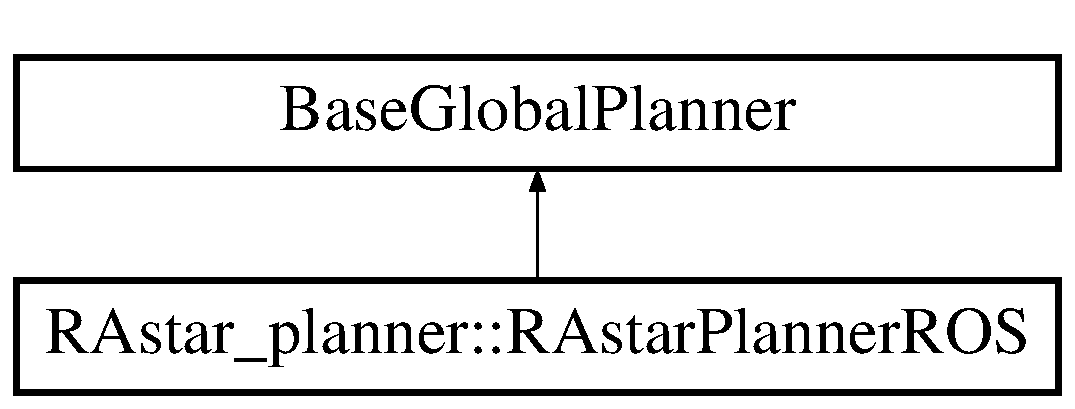
\includegraphics[height=2.000000cm]{db/dde/classRAstar__planner_1_1RAstarPlannerROS}
\end{center}
\end{figure}
\subsection*{Public Member Functions}
\begin{DoxyCompactItemize}
\item 
\hyperlink{classRAstar__planner_1_1RAstarPlannerROS_a7ab03997ec15cc3f6ad7bf9969ba8a5d}{R\-Astar\-Planner\-R\-O\-S} (ros\-::\-Node\-Handle \&)
\item 
\hyperlink{classRAstar__planner_1_1RAstarPlannerROS_a2fdd3733c0497e0ca8f5b248aec214c5}{R\-Astar\-Planner\-R\-O\-S} ()
\item 
\hyperlink{classRAstar__planner_1_1RAstarPlannerROS_abc05123045762f13f17b45d0c491034b}{R\-Astar\-Planner\-R\-O\-S} (std\-::string name, costmap\-\_\-2d\-::\-Costmap2\-D\-R\-O\-S $\ast$costmap\-\_\-ros)
\item 
void \hyperlink{classRAstar__planner_1_1RAstarPlannerROS_aed71ff1907cf853c7e49e78d3f82a94b}{initialize} (std\-::string name, costmap\-\_\-2d\-::\-Costmap2\-D\-R\-O\-S $\ast$costmap\-\_\-ros)
\begin{DoxyCompactList}\small\item\em Initialize planner. \end{DoxyCompactList}\item 
bool \hyperlink{classRAstar__planner_1_1RAstarPlannerROS_acdc8059b6324f030c47ec2322f69f658}{make\-Plan} (const geometry\-\_\-msgs\-::\-Pose\-Stamped \&start, const geometry\-\_\-msgs\-::\-Pose\-Stamped \&goal, std\-::vector$<$ geometry\-\_\-msgs\-::\-Pose\-Stamped $>$ \&plan)
\begin{DoxyCompactList}\small\item\em Create a plan given a start and goal. \end{DoxyCompactList}\item 
void \hyperlink{classRAstar__planner_1_1RAstarPlannerROS_abbc4c3daf28590f0d5e45c8227b7ff9e}{get\-Corrdinate} (float \&x, float \&y)
\begin{DoxyCompactList}\small\item\em Get cooridnate based on x,y position and origin location. \end{DoxyCompactList}\item 
int \hyperlink{classRAstar__planner_1_1RAstarPlannerROS_a50f7adc635522b9ea7f5348870b7ca6e}{convert\-To\-Cell\-Index} (float x, float y)
\begin{DoxyCompactList}\small\item\em Get cell index based on x,y and resolution. \end{DoxyCompactList}\item 
void \hyperlink{classRAstar__planner_1_1RAstarPlannerROS_a1046296d428b694e517ef25cac423846}{convert\-To\-Coordinate} (int index, float \&x, float \&y)
\begin{DoxyCompactList}\small\item\em Convert to coordinate base on x,y, origin location, and id index. \end{DoxyCompactList}\item 
bool \hyperlink{classRAstar__planner_1_1RAstarPlannerROS_a1d3f1b7aed836e648645dd696823193b}{is\-Cell\-Inside\-Map} (float x, float y)
\begin{DoxyCompactList}\small\item\em Check if cell is in the map based on resolution, width, and height of map. \end{DoxyCompactList}\item 
void \hyperlink{classRAstar__planner_1_1RAstarPlannerROS_a5bb178849971d2425519d247874cfbd9}{map\-To\-World} (double mx, double my, double \&wx, double \&wy)
\begin{DoxyCompactList}\small\item\em Convert costmap to world coordinates based on origin and resolution. \end{DoxyCompactList}\item 
vector$<$ int $>$ \hyperlink{classRAstar__planner_1_1RAstarPlannerROS_a645d6e916622ae9151721dd5188389b9}{R\-Astar\-Planner} (int start\-Cell, int goal\-Cell)
\begin{DoxyCompactList}\small\item\em Find best path from start to goal and time how long it took. \end{DoxyCompactList}\item 
vector$<$ int $>$ \hyperlink{classRAstar__planner_1_1RAstarPlannerROS_af76635e270a26e8e3da8fa9a9c228377}{find\-Path} (int start\-Cell, int goal\-Cell, float g\-\_\-score\mbox{[}$\,$\mbox{]})
\begin{DoxyCompactList}\small\item\em Run through algorithm to find path to goal, update open list and cost scores. \end{DoxyCompactList}\item 
vector$<$ int $>$ \hyperlink{classRAstar__planner_1_1RAstarPlannerROS_a6976421411cfe98a8d426d6f9c68f436}{construct\-Path} (int start\-Cell, int goal\-Cell, float g\-\_\-score\mbox{[}$\,$\mbox{]})
\begin{DoxyCompactList}\small\item\em Construct the path given start, goal, and gscores from find\-Path. \end{DoxyCompactList}\item 
float \hyperlink{classRAstar__planner_1_1RAstarPlannerROS_a723d289d6debbf185e8a0e8430a0a4d7}{calculate\-H\-Cost} (int cell\-I\-D, int goal\-Cell)
\begin{DoxyCompactList}\small\item\em Calculate Heuristic cost. \end{DoxyCompactList}\item 
void \hyperlink{classRAstar__planner_1_1RAstarPlannerROS_a16d9f8d214db7aa9c42faade56580b83}{add\-Neighbor\-Cell\-To\-Open\-List} (multiset$<$ \hyperlink{structcells}{cells} $>$ \&O\-P\-L, int neighbor\-Cell, int goal\-Cell, float g\-\_\-score\mbox{[}$\,$\mbox{]})
\begin{DoxyCompactList}\small\item\em Add a cell to the Open List. \end{DoxyCompactList}\item 
vector$<$ int $>$ \hyperlink{classRAstar__planner_1_1RAstarPlannerROS_a1923be37fd592c26b7862a694aaa1cd4}{find\-Free\-Neighbor\-Cell} (int Cell\-I\-D)
\begin{DoxyCompactList}\small\item\em Find free neighbors of current cell. \end{DoxyCompactList}\item 
bool \hyperlink{classRAstar__planner_1_1RAstarPlannerROS_a6c34ac7de619dc756a8598f8e81bfaac}{is\-Start\-And\-Goal\-Cells\-Valid} (int start\-Cell, int goal\-Cell)
\begin{DoxyCompactList}\small\item\em Checks if start and goal are valid cells. \end{DoxyCompactList}\item 
float \hyperlink{classRAstar__planner_1_1RAstarPlannerROS_a2835ea7684c39af99ce0f6acdb6b16ac}{get\-Move\-Cost} (int Cell\-I\-D1, int Cell\-I\-D2)
\begin{DoxyCompactList}\small\item\em Get the cost given two cell Ids. Get points and use other get\-Move\-Cost function. \end{DoxyCompactList}\item 
float \hyperlink{classRAstar__planner_1_1RAstarPlannerROS_adf21053b27e33f30df2dea62f910481c}{get\-Move\-Cost} (int i1, int j1, int i2, int j2)
\begin{DoxyCompactList}\small\item\em Get the move cost given two cells, four points (x,y) \end{DoxyCompactList}\item 
bool \hyperlink{classRAstar__planner_1_1RAstarPlannerROS_a2993e43fb09446c21df27735986e13c1}{is\-Free} (int Cell\-I\-D)
\begin{DoxyCompactList}\small\item\em Check if a cell is free from cell I\-D. \end{DoxyCompactList}\item 
bool \hyperlink{classRAstar__planner_1_1RAstarPlannerROS_a1648d66652edcba3b73284af7f5b7c18}{is\-Free} (int i, int j)
\begin{DoxyCompactList}\small\item\em Check if a cell is free from i,j point. \end{DoxyCompactList}\item 
int \hyperlink{classRAstar__planner_1_1RAstarPlannerROS_ade7b3d65aa5e97588a58e968852cc279}{get\-Cell\-Index} (int i, int j)
\begin{DoxyCompactList}\small\item\em Get cell index from point i,j and width. \end{DoxyCompactList}\item 
int \hyperlink{classRAstar__planner_1_1RAstarPlannerROS_af17757b32cb946011d64fa9478395bdf}{get\-Cell\-Row\-I\-D} (int index)
\begin{DoxyCompactList}\small\item\em Get row id for cell given index, using width. \end{DoxyCompactList}\item 
int \hyperlink{classRAstar__planner_1_1RAstarPlannerROS_ae6ea4452952f573c9554b9680c2e9d3d}{get\-Cell\-Col\-I\-D} (int index)
\begin{DoxyCompactList}\small\item\em Get column id for cell given index, using width. \end{DoxyCompactList}\item 
void \hyperlink{classRAstar__planner_1_1RAstarPlannerROS_a0ea613cb0c57682fd0ce840bbf5ed1d5}{publish\-Plan} (const std\-::vector$<$ geometry\-\_\-msgs\-::\-Pose\-Stamped $>$ \&path, double r, double g, double b, double a)
\begin{DoxyCompactList}\small\item\em Publish the final path. \end{DoxyCompactList}\end{DoxyCompactItemize}
\subsection*{Public Attributes}
\begin{DoxyCompactItemize}
\item 
ros\-::\-Publisher \hyperlink{classRAstar__planner_1_1RAstarPlannerROS_a53d1415cf583098e3e9444d6258e1677}{plan\-\_\-pub\-\_\-}
\item 
ros\-::\-Node\-Handle \hyperlink{classRAstar__planner_1_1RAstarPlannerROS_a7371972d6a02e857f3640b795c5ef11c}{R\-O\-S\-Node\-Handle}
\item 
float \hyperlink{classRAstar__planner_1_1RAstarPlannerROS_ad2259dddb7800340bc6d5f89ebc4186b}{origin\-X}
\item 
float \hyperlink{classRAstar__planner_1_1RAstarPlannerROS_a94427d193482b1c34b3db7ae2bfb8155}{origin\-Y}
\item 
float \hyperlink{classRAstar__planner_1_1RAstarPlannerROS_a651c37170c82d3b116961a9ba1ccea6e}{resolution}
\item 
costmap\-\_\-2d\-::\-Costmap2\-D\-R\-O\-S $\ast$ \hyperlink{classRAstar__planner_1_1RAstarPlannerROS_a7bec96cd0f94ecb17f98e206e46e461b}{costmap\-\_\-ros\-\_\-}
\item 
double \hyperlink{classRAstar__planner_1_1RAstarPlannerROS_ab9efb9a5f82f7c82c91f438c05a22c91}{step\-\_\-size\-\_\-}
\item 
double \hyperlink{classRAstar__planner_1_1RAstarPlannerROS_a0dc442aa982d3fdedb8dbbc22b28a470}{min\-\_\-dist\-\_\-from\-\_\-robot\-\_\-}
\item 
costmap\-\_\-2d\-::\-Costmap2\-D $\ast$ \hyperlink{classRAstar__planner_1_1RAstarPlannerROS_a8e9d61f1082f16a9bedb7f038fa090ed}{costmap\-\_\-}
\item 
bool \hyperlink{classRAstar__planner_1_1RAstarPlannerROS_a01c6678d519c4f7667747ea21dccd8ba}{initialized\-\_\-}
\item 
int \hyperlink{classRAstar__planner_1_1RAstarPlannerROS_accbb5d01b9d9630eb906c71fb255dd0d}{width}
\item 
int \hyperlink{classRAstar__planner_1_1RAstarPlannerROS_ab200f89722ca863dff4daf8ea25fd910}{height}
\item 
bool $\ast$ \hyperlink{classRAstar__planner_1_1RAstarPlannerROS_a873e16d6355ad94a276f4795bb450141}{O\-G\-M}
\end{DoxyCompactItemize}


\subsection{Constructor \& Destructor Documentation}
\hypertarget{classRAstar__planner_1_1RAstarPlannerROS_a7ab03997ec15cc3f6ad7bf9969ba8a5d}{\index{R\-Astar\-\_\-planner\-::\-R\-Astar\-Planner\-R\-O\-S@{R\-Astar\-\_\-planner\-::\-R\-Astar\-Planner\-R\-O\-S}!R\-Astar\-Planner\-R\-O\-S@{R\-Astar\-Planner\-R\-O\-S}}
\index{R\-Astar\-Planner\-R\-O\-S@{R\-Astar\-Planner\-R\-O\-S}!RAstar_planner::RAstarPlannerROS@{R\-Astar\-\_\-planner\-::\-R\-Astar\-Planner\-R\-O\-S}}
\subsubsection[{R\-Astar\-Planner\-R\-O\-S}]{\setlength{\rightskip}{0pt plus 5cm}R\-Astar\-\_\-planner\-::\-R\-Astar\-Planner\-R\-O\-S\-::\-R\-Astar\-Planner\-R\-O\-S (
\begin{DoxyParamCaption}
\item[{ros\-::\-Node\-Handle \&}]{}
\end{DoxyParamCaption}
)\hspace{0.3cm}{\ttfamily [explicit]}}}\label{classRAstar__planner_1_1RAstarPlannerROS_a7ab03997ec15cc3f6ad7bf9969ba8a5d}
\hypertarget{classRAstar__planner_1_1RAstarPlannerROS_a2fdd3733c0497e0ca8f5b248aec214c5}{\index{R\-Astar\-\_\-planner\-::\-R\-Astar\-Planner\-R\-O\-S@{R\-Astar\-\_\-planner\-::\-R\-Astar\-Planner\-R\-O\-S}!R\-Astar\-Planner\-R\-O\-S@{R\-Astar\-Planner\-R\-O\-S}}
\index{R\-Astar\-Planner\-R\-O\-S@{R\-Astar\-Planner\-R\-O\-S}!RAstar_planner::RAstarPlannerROS@{R\-Astar\-\_\-planner\-::\-R\-Astar\-Planner\-R\-O\-S}}
\subsubsection[{R\-Astar\-Planner\-R\-O\-S}]{\setlength{\rightskip}{0pt plus 5cm}R\-Astar\-\_\-planner\-::\-R\-Astar\-Planner\-R\-O\-S\-::\-R\-Astar\-Planner\-R\-O\-S (
\begin{DoxyParamCaption}
{}
\end{DoxyParamCaption}
)}}\label{classRAstar__planner_1_1RAstarPlannerROS_a2fdd3733c0497e0ca8f5b248aec214c5}
\hypertarget{classRAstar__planner_1_1RAstarPlannerROS_abc05123045762f13f17b45d0c491034b}{\index{R\-Astar\-\_\-planner\-::\-R\-Astar\-Planner\-R\-O\-S@{R\-Astar\-\_\-planner\-::\-R\-Astar\-Planner\-R\-O\-S}!R\-Astar\-Planner\-R\-O\-S@{R\-Astar\-Planner\-R\-O\-S}}
\index{R\-Astar\-Planner\-R\-O\-S@{R\-Astar\-Planner\-R\-O\-S}!RAstar_planner::RAstarPlannerROS@{R\-Astar\-\_\-planner\-::\-R\-Astar\-Planner\-R\-O\-S}}
\subsubsection[{R\-Astar\-Planner\-R\-O\-S}]{\setlength{\rightskip}{0pt plus 5cm}R\-Astar\-\_\-planner\-::\-R\-Astar\-Planner\-R\-O\-S\-::\-R\-Astar\-Planner\-R\-O\-S (
\begin{DoxyParamCaption}
\item[{std\-::string}]{name, }
\item[{costmap\-\_\-2d\-::\-Costmap2\-D\-R\-O\-S $\ast$}]{costmap\-\_\-ros}
\end{DoxyParamCaption}
)}}\label{classRAstar__planner_1_1RAstarPlannerROS_abc05123045762f13f17b45d0c491034b}


\subsection{Member Function Documentation}
\hypertarget{classRAstar__planner_1_1RAstarPlannerROS_a16d9f8d214db7aa9c42faade56580b83}{\index{R\-Astar\-\_\-planner\-::\-R\-Astar\-Planner\-R\-O\-S@{R\-Astar\-\_\-planner\-::\-R\-Astar\-Planner\-R\-O\-S}!add\-Neighbor\-Cell\-To\-Open\-List@{add\-Neighbor\-Cell\-To\-Open\-List}}
\index{add\-Neighbor\-Cell\-To\-Open\-List@{add\-Neighbor\-Cell\-To\-Open\-List}!RAstar_planner::RAstarPlannerROS@{R\-Astar\-\_\-planner\-::\-R\-Astar\-Planner\-R\-O\-S}}
\subsubsection[{add\-Neighbor\-Cell\-To\-Open\-List}]{\setlength{\rightskip}{0pt plus 5cm}void R\-Astar\-\_\-planner\-::\-R\-Astar\-Planner\-R\-O\-S\-::add\-Neighbor\-Cell\-To\-Open\-List (
\begin{DoxyParamCaption}
\item[{multiset$<$ {\bf cells} $>$ \&}]{O\-P\-L, }
\item[{int}]{neighbor\-Cell, }
\item[{int}]{goal\-Cell, }
\item[{float}]{g\-\_\-score\mbox{[}$\,$\mbox{]}}
\end{DoxyParamCaption}
)}}\label{classRAstar__planner_1_1RAstarPlannerROS_a16d9f8d214db7aa9c42faade56580b83}


Add a cell to the Open List. 


\begin{DoxyParams}{Parameters}
{\em O\-P\-L} & in multiset cells \\
\hline
{\em neighbor\-Cell} & in int \\
\hline
{\em goal\-Cell} & in int \\
\hline
{\em g\-\_\-score} & in float \\
\hline
\end{DoxyParams}
\begin{DoxyReturn}{Returns}
none 
\end{DoxyReturn}
\hypertarget{classRAstar__planner_1_1RAstarPlannerROS_a723d289d6debbf185e8a0e8430a0a4d7}{\index{R\-Astar\-\_\-planner\-::\-R\-Astar\-Planner\-R\-O\-S@{R\-Astar\-\_\-planner\-::\-R\-Astar\-Planner\-R\-O\-S}!calculate\-H\-Cost@{calculate\-H\-Cost}}
\index{calculate\-H\-Cost@{calculate\-H\-Cost}!RAstar_planner::RAstarPlannerROS@{R\-Astar\-\_\-planner\-::\-R\-Astar\-Planner\-R\-O\-S}}
\subsubsection[{calculate\-H\-Cost}]{\setlength{\rightskip}{0pt plus 5cm}float R\-Astar\-\_\-planner\-::\-R\-Astar\-Planner\-R\-O\-S\-::calculate\-H\-Cost (
\begin{DoxyParamCaption}
\item[{int}]{cell\-I\-D, }
\item[{int}]{goal\-Cell}
\end{DoxyParamCaption}
)}}\label{classRAstar__planner_1_1RAstarPlannerROS_a723d289d6debbf185e8a0e8430a0a4d7}


Calculate Heuristic cost. 


\begin{DoxyParams}{Parameters}
{\em cell\-I\-D} & in int \\
\hline
{\em goal\-Cell} & in int\\
\hline
\end{DoxyParams}
\begin{DoxyReturn}{Returns}
float Hueristic cost 
\end{DoxyReturn}
\hypertarget{classRAstar__planner_1_1RAstarPlannerROS_a6976421411cfe98a8d426d6f9c68f436}{\index{R\-Astar\-\_\-planner\-::\-R\-Astar\-Planner\-R\-O\-S@{R\-Astar\-\_\-planner\-::\-R\-Astar\-Planner\-R\-O\-S}!construct\-Path@{construct\-Path}}
\index{construct\-Path@{construct\-Path}!RAstar_planner::RAstarPlannerROS@{R\-Astar\-\_\-planner\-::\-R\-Astar\-Planner\-R\-O\-S}}
\subsubsection[{construct\-Path}]{\setlength{\rightskip}{0pt plus 5cm}vector$<$int$>$ R\-Astar\-\_\-planner\-::\-R\-Astar\-Planner\-R\-O\-S\-::construct\-Path (
\begin{DoxyParamCaption}
\item[{int}]{start\-Cell, }
\item[{int}]{goal\-Cell, }
\item[{float}]{g\-\_\-score\mbox{[}$\,$\mbox{]}}
\end{DoxyParamCaption}
)}}\label{classRAstar__planner_1_1RAstarPlannerROS_a6976421411cfe98a8d426d6f9c68f436}


Construct the path given start, goal, and gscores from find\-Path. 


\begin{DoxyParams}{Parameters}
{\em start\-Cell} & in int \\
\hline
{\em goal\-Cell} & in int \\
\hline
{\em g\-\_\-score} & in float \\
\hline
\end{DoxyParams}
\begin{DoxyReturn}{Returns}
best\-Path in vector int 
\end{DoxyReturn}
\hypertarget{classRAstar__planner_1_1RAstarPlannerROS_a50f7adc635522b9ea7f5348870b7ca6e}{\index{R\-Astar\-\_\-planner\-::\-R\-Astar\-Planner\-R\-O\-S@{R\-Astar\-\_\-planner\-::\-R\-Astar\-Planner\-R\-O\-S}!convert\-To\-Cell\-Index@{convert\-To\-Cell\-Index}}
\index{convert\-To\-Cell\-Index@{convert\-To\-Cell\-Index}!RAstar_planner::RAstarPlannerROS@{R\-Astar\-\_\-planner\-::\-R\-Astar\-Planner\-R\-O\-S}}
\subsubsection[{convert\-To\-Cell\-Index}]{\setlength{\rightskip}{0pt plus 5cm}int R\-Astar\-\_\-planner\-::\-R\-Astar\-Planner\-R\-O\-S\-::convert\-To\-Cell\-Index (
\begin{DoxyParamCaption}
\item[{float}]{x, }
\item[{float}]{y}
\end{DoxyParamCaption}
)}}\label{classRAstar__planner_1_1RAstarPlannerROS_a50f7adc635522b9ea7f5348870b7ca6e}


Get cell index based on x,y and resolution. 


\begin{DoxyParams}{Parameters}
{\em x} & in float \\
\hline
{\em y} & in float\\
\hline
\end{DoxyParams}
\begin{DoxyReturn}{Returns}
cell index in int 
\end{DoxyReturn}
\hypertarget{classRAstar__planner_1_1RAstarPlannerROS_a1046296d428b694e517ef25cac423846}{\index{R\-Astar\-\_\-planner\-::\-R\-Astar\-Planner\-R\-O\-S@{R\-Astar\-\_\-planner\-::\-R\-Astar\-Planner\-R\-O\-S}!convert\-To\-Coordinate@{convert\-To\-Coordinate}}
\index{convert\-To\-Coordinate@{convert\-To\-Coordinate}!RAstar_planner::RAstarPlannerROS@{R\-Astar\-\_\-planner\-::\-R\-Astar\-Planner\-R\-O\-S}}
\subsubsection[{convert\-To\-Coordinate}]{\setlength{\rightskip}{0pt plus 5cm}void R\-Astar\-\_\-planner\-::\-R\-Astar\-Planner\-R\-O\-S\-::convert\-To\-Coordinate (
\begin{DoxyParamCaption}
\item[{int}]{index, }
\item[{float \&}]{x, }
\item[{float \&}]{y}
\end{DoxyParamCaption}
)}}\label{classRAstar__planner_1_1RAstarPlannerROS_a1046296d428b694e517ef25cac423846}


Convert to coordinate base on x,y, origin location, and id index. 


\begin{DoxyParams}{Parameters}
{\em index} & in int \\
\hline
{\em x} & in float \\
\hline
{\em y} & in float \\
\hline
\end{DoxyParams}
\begin{DoxyReturn}{Returns}
none 
\end{DoxyReturn}
\hypertarget{classRAstar__planner_1_1RAstarPlannerROS_a1923be37fd592c26b7862a694aaa1cd4}{\index{R\-Astar\-\_\-planner\-::\-R\-Astar\-Planner\-R\-O\-S@{R\-Astar\-\_\-planner\-::\-R\-Astar\-Planner\-R\-O\-S}!find\-Free\-Neighbor\-Cell@{find\-Free\-Neighbor\-Cell}}
\index{find\-Free\-Neighbor\-Cell@{find\-Free\-Neighbor\-Cell}!RAstar_planner::RAstarPlannerROS@{R\-Astar\-\_\-planner\-::\-R\-Astar\-Planner\-R\-O\-S}}
\subsubsection[{find\-Free\-Neighbor\-Cell}]{\setlength{\rightskip}{0pt plus 5cm}vector$<$int$>$ R\-Astar\-\_\-planner\-::\-R\-Astar\-Planner\-R\-O\-S\-::find\-Free\-Neighbor\-Cell (
\begin{DoxyParamCaption}
\item[{int}]{Cell\-I\-D}
\end{DoxyParamCaption}
)}}\label{classRAstar__planner_1_1RAstarPlannerROS_a1923be37fd592c26b7862a694aaa1cd4}


Find free neighbors of current cell. 


\begin{DoxyParams}{Parameters}
{\em cell\-I\-D} & in int \\
\hline
\end{DoxyParams}
\begin{DoxyReturn}{Returns}
Free neighbors cells in vector int 
\end{DoxyReturn}
\hypertarget{classRAstar__planner_1_1RAstarPlannerROS_af76635e270a26e8e3da8fa9a9c228377}{\index{R\-Astar\-\_\-planner\-::\-R\-Astar\-Planner\-R\-O\-S@{R\-Astar\-\_\-planner\-::\-R\-Astar\-Planner\-R\-O\-S}!find\-Path@{find\-Path}}
\index{find\-Path@{find\-Path}!RAstar_planner::RAstarPlannerROS@{R\-Astar\-\_\-planner\-::\-R\-Astar\-Planner\-R\-O\-S}}
\subsubsection[{find\-Path}]{\setlength{\rightskip}{0pt plus 5cm}vector$<$int$>$ R\-Astar\-\_\-planner\-::\-R\-Astar\-Planner\-R\-O\-S\-::find\-Path (
\begin{DoxyParamCaption}
\item[{int}]{start\-Cell, }
\item[{int}]{goal\-Cell, }
\item[{float}]{g\-\_\-score\mbox{[}$\,$\mbox{]}}
\end{DoxyParamCaption}
)}}\label{classRAstar__planner_1_1RAstarPlannerROS_af76635e270a26e8e3da8fa9a9c228377}


Run through algorithm to find path to goal, update open list and cost scores. 


\begin{DoxyParams}{Parameters}
{\em start\-Cell} & in int \\
\hline
{\em goal\-Cell} & in int \\
\hline
{\em g\-\_\-score} & in float \\
\hline
\end{DoxyParams}
\begin{DoxyReturn}{Returns}
best\-Path in vector int 
\end{DoxyReturn}
\hypertarget{classRAstar__planner_1_1RAstarPlannerROS_ae6ea4452952f573c9554b9680c2e9d3d}{\index{R\-Astar\-\_\-planner\-::\-R\-Astar\-Planner\-R\-O\-S@{R\-Astar\-\_\-planner\-::\-R\-Astar\-Planner\-R\-O\-S}!get\-Cell\-Col\-I\-D@{get\-Cell\-Col\-I\-D}}
\index{get\-Cell\-Col\-I\-D@{get\-Cell\-Col\-I\-D}!RAstar_planner::RAstarPlannerROS@{R\-Astar\-\_\-planner\-::\-R\-Astar\-Planner\-R\-O\-S}}
\subsubsection[{get\-Cell\-Col\-I\-D}]{\setlength{\rightskip}{0pt plus 5cm}int R\-Astar\-\_\-planner\-::\-R\-Astar\-Planner\-R\-O\-S\-::get\-Cell\-Col\-I\-D (
\begin{DoxyParamCaption}
\item[{int}]{index}
\end{DoxyParamCaption}
)}}\label{classRAstar__planner_1_1RAstarPlannerROS_ae6ea4452952f573c9554b9680c2e9d3d}


Get column id for cell given index, using width. 


\begin{DoxyParams}{Parameters}
{\em index} & in int \\
\hline
\end{DoxyParams}
\begin{DoxyReturn}{Returns}
cell column id in int 
\end{DoxyReturn}
\hypertarget{classRAstar__planner_1_1RAstarPlannerROS_ade7b3d65aa5e97588a58e968852cc279}{\index{R\-Astar\-\_\-planner\-::\-R\-Astar\-Planner\-R\-O\-S@{R\-Astar\-\_\-planner\-::\-R\-Astar\-Planner\-R\-O\-S}!get\-Cell\-Index@{get\-Cell\-Index}}
\index{get\-Cell\-Index@{get\-Cell\-Index}!RAstar_planner::RAstarPlannerROS@{R\-Astar\-\_\-planner\-::\-R\-Astar\-Planner\-R\-O\-S}}
\subsubsection[{get\-Cell\-Index}]{\setlength{\rightskip}{0pt plus 5cm}int R\-Astar\-\_\-planner\-::\-R\-Astar\-Planner\-R\-O\-S\-::get\-Cell\-Index (
\begin{DoxyParamCaption}
\item[{int}]{i, }
\item[{int}]{j}
\end{DoxyParamCaption}
)}}\label{classRAstar__planner_1_1RAstarPlannerROS_ade7b3d65aa5e97588a58e968852cc279}


Get cell index from point i,j and width. 


\begin{DoxyParams}{Parameters}
{\em i} & in int \\
\hline
{\em j} & in int \\
\hline
\end{DoxyParams}
\begin{DoxyReturn}{Returns}
cell index in int 
\end{DoxyReturn}
\hypertarget{classRAstar__planner_1_1RAstarPlannerROS_af17757b32cb946011d64fa9478395bdf}{\index{R\-Astar\-\_\-planner\-::\-R\-Astar\-Planner\-R\-O\-S@{R\-Astar\-\_\-planner\-::\-R\-Astar\-Planner\-R\-O\-S}!get\-Cell\-Row\-I\-D@{get\-Cell\-Row\-I\-D}}
\index{get\-Cell\-Row\-I\-D@{get\-Cell\-Row\-I\-D}!RAstar_planner::RAstarPlannerROS@{R\-Astar\-\_\-planner\-::\-R\-Astar\-Planner\-R\-O\-S}}
\subsubsection[{get\-Cell\-Row\-I\-D}]{\setlength{\rightskip}{0pt plus 5cm}int R\-Astar\-\_\-planner\-::\-R\-Astar\-Planner\-R\-O\-S\-::get\-Cell\-Row\-I\-D (
\begin{DoxyParamCaption}
\item[{int}]{index}
\end{DoxyParamCaption}
)}}\label{classRAstar__planner_1_1RAstarPlannerROS_af17757b32cb946011d64fa9478395bdf}


Get row id for cell given index, using width. 


\begin{DoxyParams}{Parameters}
{\em index} & in int \\
\hline
\end{DoxyParams}
\begin{DoxyReturn}{Returns}
cell row id in int 
\end{DoxyReturn}
\hypertarget{classRAstar__planner_1_1RAstarPlannerROS_abbc4c3daf28590f0d5e45c8227b7ff9e}{\index{R\-Astar\-\_\-planner\-::\-R\-Astar\-Planner\-R\-O\-S@{R\-Astar\-\_\-planner\-::\-R\-Astar\-Planner\-R\-O\-S}!get\-Corrdinate@{get\-Corrdinate}}
\index{get\-Corrdinate@{get\-Corrdinate}!RAstar_planner::RAstarPlannerROS@{R\-Astar\-\_\-planner\-::\-R\-Astar\-Planner\-R\-O\-S}}
\subsubsection[{get\-Corrdinate}]{\setlength{\rightskip}{0pt plus 5cm}void R\-Astar\-\_\-planner\-::\-R\-Astar\-Planner\-R\-O\-S\-::get\-Corrdinate (
\begin{DoxyParamCaption}
\item[{float \&}]{x, }
\item[{float \&}]{y}
\end{DoxyParamCaption}
)}}\label{classRAstar__planner_1_1RAstarPlannerROS_abbc4c3daf28590f0d5e45c8227b7ff9e}


Get cooridnate based on x,y position and origin location. 


\begin{DoxyParams}{Parameters}
{\em x} & in float \\
\hline
{\em y} & in float\\
\hline
\end{DoxyParams}
\begin{DoxyReturn}{Returns}
none 
\end{DoxyReturn}
\hypertarget{classRAstar__planner_1_1RAstarPlannerROS_a2835ea7684c39af99ce0f6acdb6b16ac}{\index{R\-Astar\-\_\-planner\-::\-R\-Astar\-Planner\-R\-O\-S@{R\-Astar\-\_\-planner\-::\-R\-Astar\-Planner\-R\-O\-S}!get\-Move\-Cost@{get\-Move\-Cost}}
\index{get\-Move\-Cost@{get\-Move\-Cost}!RAstar_planner::RAstarPlannerROS@{R\-Astar\-\_\-planner\-::\-R\-Astar\-Planner\-R\-O\-S}}
\subsubsection[{get\-Move\-Cost}]{\setlength{\rightskip}{0pt plus 5cm}float R\-Astar\-\_\-planner\-::\-R\-Astar\-Planner\-R\-O\-S\-::get\-Move\-Cost (
\begin{DoxyParamCaption}
\item[{int}]{Cell\-I\-D1, }
\item[{int}]{Cell\-I\-D2}
\end{DoxyParamCaption}
)}}\label{classRAstar__planner_1_1RAstarPlannerROS_a2835ea7684c39af99ce0f6acdb6b16ac}


Get the cost given two cell Ids. Get points and use other get\-Move\-Cost function. 


\begin{DoxyParams}{Parameters}
{\em Cell\-I\-D1} & in int \\
\hline
{\em cell\-I\-D2} & in int \\
\hline
\end{DoxyParams}
\begin{DoxyReturn}{Returns}
move\-Cost in float 
\end{DoxyReturn}
\hypertarget{classRAstar__planner_1_1RAstarPlannerROS_adf21053b27e33f30df2dea62f910481c}{\index{R\-Astar\-\_\-planner\-::\-R\-Astar\-Planner\-R\-O\-S@{R\-Astar\-\_\-planner\-::\-R\-Astar\-Planner\-R\-O\-S}!get\-Move\-Cost@{get\-Move\-Cost}}
\index{get\-Move\-Cost@{get\-Move\-Cost}!RAstar_planner::RAstarPlannerROS@{R\-Astar\-\_\-planner\-::\-R\-Astar\-Planner\-R\-O\-S}}
\subsubsection[{get\-Move\-Cost}]{\setlength{\rightskip}{0pt plus 5cm}float R\-Astar\-\_\-planner\-::\-R\-Astar\-Planner\-R\-O\-S\-::get\-Move\-Cost (
\begin{DoxyParamCaption}
\item[{int}]{i1, }
\item[{int}]{j1, }
\item[{int}]{i2, }
\item[{int}]{j2}
\end{DoxyParamCaption}
)}}\label{classRAstar__planner_1_1RAstarPlannerROS_adf21053b27e33f30df2dea62f910481c}


Get the move cost given two cells, four points (x,y) 


\begin{DoxyParams}{Parameters}
{\em i1} & in int \\
\hline
{\em j1} & in int \\
\hline
{\em i2} & in int \\
\hline
{\em j2} & in int \\
\hline
\end{DoxyParams}
\begin{DoxyReturn}{Returns}
move\-Cost in float 
\end{DoxyReturn}
\hypertarget{classRAstar__planner_1_1RAstarPlannerROS_aed71ff1907cf853c7e49e78d3f82a94b}{\index{R\-Astar\-\_\-planner\-::\-R\-Astar\-Planner\-R\-O\-S@{R\-Astar\-\_\-planner\-::\-R\-Astar\-Planner\-R\-O\-S}!initialize@{initialize}}
\index{initialize@{initialize}!RAstar_planner::RAstarPlannerROS@{R\-Astar\-\_\-planner\-::\-R\-Astar\-Planner\-R\-O\-S}}
\subsubsection[{initialize}]{\setlength{\rightskip}{0pt plus 5cm}void R\-Astar\-\_\-planner\-::\-R\-Astar\-Planner\-R\-O\-S\-::initialize (
\begin{DoxyParamCaption}
\item[{std\-::string}]{name, }
\item[{costmap\-\_\-2d\-::\-Costmap2\-D\-R\-O\-S $\ast$}]{costmap\-\_\-ros}
\end{DoxyParamCaption}
)}}\label{classRAstar__planner_1_1RAstarPlannerROS_aed71ff1907cf853c7e49e78d3f82a94b}


Initialize planner. 

overriden classes from interface nav\-\_\-core\-::\-Base\-Global\-Planner 
\begin{DoxyParams}{Parameters}
{\em name} & in string \\
\hline
{\em costmap} & from costmap\-\_\-2s\-::\-Costmap2\-D\-R\-O\-S \\
\hline
\end{DoxyParams}
\begin{DoxyReturn}{Returns}
none 
\end{DoxyReturn}
\hypertarget{classRAstar__planner_1_1RAstarPlannerROS_a1d3f1b7aed836e648645dd696823193b}{\index{R\-Astar\-\_\-planner\-::\-R\-Astar\-Planner\-R\-O\-S@{R\-Astar\-\_\-planner\-::\-R\-Astar\-Planner\-R\-O\-S}!is\-Cell\-Inside\-Map@{is\-Cell\-Inside\-Map}}
\index{is\-Cell\-Inside\-Map@{is\-Cell\-Inside\-Map}!RAstar_planner::RAstarPlannerROS@{R\-Astar\-\_\-planner\-::\-R\-Astar\-Planner\-R\-O\-S}}
\subsubsection[{is\-Cell\-Inside\-Map}]{\setlength{\rightskip}{0pt plus 5cm}bool R\-Astar\-\_\-planner\-::\-R\-Astar\-Planner\-R\-O\-S\-::is\-Cell\-Inside\-Map (
\begin{DoxyParamCaption}
\item[{float}]{x, }
\item[{float}]{y}
\end{DoxyParamCaption}
)}}\label{classRAstar__planner_1_1RAstarPlannerROS_a1d3f1b7aed836e648645dd696823193b}


Check if cell is in the map based on resolution, width, and height of map. 


\begin{DoxyParams}{Parameters}
{\em float} & in x \\
\hline
{\em float} & in y\\
\hline
\end{DoxyParams}
\begin{DoxyReturn}{Returns}
true/false 
\end{DoxyReturn}
\hypertarget{classRAstar__planner_1_1RAstarPlannerROS_a2993e43fb09446c21df27735986e13c1}{\index{R\-Astar\-\_\-planner\-::\-R\-Astar\-Planner\-R\-O\-S@{R\-Astar\-\_\-planner\-::\-R\-Astar\-Planner\-R\-O\-S}!is\-Free@{is\-Free}}
\index{is\-Free@{is\-Free}!RAstar_planner::RAstarPlannerROS@{R\-Astar\-\_\-planner\-::\-R\-Astar\-Planner\-R\-O\-S}}
\subsubsection[{is\-Free}]{\setlength{\rightskip}{0pt plus 5cm}bool R\-Astar\-\_\-planner\-::\-R\-Astar\-Planner\-R\-O\-S\-::is\-Free (
\begin{DoxyParamCaption}
\item[{int}]{Cell\-I\-D}
\end{DoxyParamCaption}
)}}\label{classRAstar__planner_1_1RAstarPlannerROS_a2993e43fb09446c21df27735986e13c1}


Check if a cell is free from cell I\-D. 


\begin{DoxyParams}{Parameters}
{\em Cell\-I\-D} & in int \\
\hline
\end{DoxyParams}
\begin{DoxyReturn}{Returns}
true/false 
\end{DoxyReturn}
\hypertarget{classRAstar__planner_1_1RAstarPlannerROS_a1648d66652edcba3b73284af7f5b7c18}{\index{R\-Astar\-\_\-planner\-::\-R\-Astar\-Planner\-R\-O\-S@{R\-Astar\-\_\-planner\-::\-R\-Astar\-Planner\-R\-O\-S}!is\-Free@{is\-Free}}
\index{is\-Free@{is\-Free}!RAstar_planner::RAstarPlannerROS@{R\-Astar\-\_\-planner\-::\-R\-Astar\-Planner\-R\-O\-S}}
\subsubsection[{is\-Free}]{\setlength{\rightskip}{0pt plus 5cm}bool R\-Astar\-\_\-planner\-::\-R\-Astar\-Planner\-R\-O\-S\-::is\-Free (
\begin{DoxyParamCaption}
\item[{int}]{i, }
\item[{int}]{j}
\end{DoxyParamCaption}
)}}\label{classRAstar__planner_1_1RAstarPlannerROS_a1648d66652edcba3b73284af7f5b7c18}


Check if a cell is free from i,j point. 


\begin{DoxyParams}{Parameters}
{\em i} & in int \\
\hline
{\em j} & in int \\
\hline
\end{DoxyParams}
\begin{DoxyReturn}{Returns}
true/false 
\end{DoxyReturn}
\hypertarget{classRAstar__planner_1_1RAstarPlannerROS_a6c34ac7de619dc756a8598f8e81bfaac}{\index{R\-Astar\-\_\-planner\-::\-R\-Astar\-Planner\-R\-O\-S@{R\-Astar\-\_\-planner\-::\-R\-Astar\-Planner\-R\-O\-S}!is\-Start\-And\-Goal\-Cells\-Valid@{is\-Start\-And\-Goal\-Cells\-Valid}}
\index{is\-Start\-And\-Goal\-Cells\-Valid@{is\-Start\-And\-Goal\-Cells\-Valid}!RAstar_planner::RAstarPlannerROS@{R\-Astar\-\_\-planner\-::\-R\-Astar\-Planner\-R\-O\-S}}
\subsubsection[{is\-Start\-And\-Goal\-Cells\-Valid}]{\setlength{\rightskip}{0pt plus 5cm}bool R\-Astar\-\_\-planner\-::\-R\-Astar\-Planner\-R\-O\-S\-::is\-Start\-And\-Goal\-Cells\-Valid (
\begin{DoxyParamCaption}
\item[{int}]{start\-Cell, }
\item[{int}]{goal\-Cell}
\end{DoxyParamCaption}
)}}\label{classRAstar__planner_1_1RAstarPlannerROS_a6c34ac7de619dc756a8598f8e81bfaac}


Checks if start and goal are valid cells. 


\begin{DoxyParams}{Parameters}
{\em start\-Cell} & in int \\
\hline
{\em goal\-Cell} & in int \\
\hline
\end{DoxyParams}
\begin{DoxyReturn}{Returns}
true/false 
\end{DoxyReturn}
\hypertarget{classRAstar__planner_1_1RAstarPlannerROS_acdc8059b6324f030c47ec2322f69f658}{\index{R\-Astar\-\_\-planner\-::\-R\-Astar\-Planner\-R\-O\-S@{R\-Astar\-\_\-planner\-::\-R\-Astar\-Planner\-R\-O\-S}!make\-Plan@{make\-Plan}}
\index{make\-Plan@{make\-Plan}!RAstar_planner::RAstarPlannerROS@{R\-Astar\-\_\-planner\-::\-R\-Astar\-Planner\-R\-O\-S}}
\subsubsection[{make\-Plan}]{\setlength{\rightskip}{0pt plus 5cm}bool R\-Astar\-\_\-planner\-::\-R\-Astar\-Planner\-R\-O\-S\-::make\-Plan (
\begin{DoxyParamCaption}
\item[{const geometry\-\_\-msgs\-::\-Pose\-Stamped \&}]{start, }
\item[{const geometry\-\_\-msgs\-::\-Pose\-Stamped \&}]{goal, }
\item[{std\-::vector$<$ geometry\-\_\-msgs\-::\-Pose\-Stamped $>$ \&}]{plan}
\end{DoxyParamCaption}
)}}\label{classRAstar__planner_1_1RAstarPlannerROS_acdc8059b6324f030c47ec2322f69f658}


Create a plan given a start and goal. 


\begin{DoxyParams}{Parameters}
{\em start} & in geometry message/\-Posestamped \\
\hline
{\em start} & in geometry message/\-Posestamped \\
\hline
{\em plan} & in vector of geometry messages/\-Posestamped \\
\hline
\end{DoxyParams}
\begin{DoxyReturn}{Returns}
true/false 
\end{DoxyReturn}
\hypertarget{classRAstar__planner_1_1RAstarPlannerROS_a5bb178849971d2425519d247874cfbd9}{\index{R\-Astar\-\_\-planner\-::\-R\-Astar\-Planner\-R\-O\-S@{R\-Astar\-\_\-planner\-::\-R\-Astar\-Planner\-R\-O\-S}!map\-To\-World@{map\-To\-World}}
\index{map\-To\-World@{map\-To\-World}!RAstar_planner::RAstarPlannerROS@{R\-Astar\-\_\-planner\-::\-R\-Astar\-Planner\-R\-O\-S}}
\subsubsection[{map\-To\-World}]{\setlength{\rightskip}{0pt plus 5cm}void R\-Astar\-\_\-planner\-::\-R\-Astar\-Planner\-R\-O\-S\-::map\-To\-World (
\begin{DoxyParamCaption}
\item[{double}]{mx, }
\item[{double}]{my, }
\item[{double \&}]{wx, }
\item[{double \&}]{wy}
\end{DoxyParamCaption}
)}}\label{classRAstar__planner_1_1RAstarPlannerROS_a5bb178849971d2425519d247874cfbd9}


Convert costmap to world coordinates based on origin and resolution. 


\begin{DoxyParams}{Parameters}
{\em mx} & in double \\
\hline
{\em my} & in double \\
\hline
{\em wx} & in double \\
\hline
{\em wy} & in double \\
\hline
\end{DoxyParams}
\begin{DoxyReturn}{Returns}
none 
\end{DoxyReturn}
\hypertarget{classRAstar__planner_1_1RAstarPlannerROS_a0ea613cb0c57682fd0ce840bbf5ed1d5}{\index{R\-Astar\-\_\-planner\-::\-R\-Astar\-Planner\-R\-O\-S@{R\-Astar\-\_\-planner\-::\-R\-Astar\-Planner\-R\-O\-S}!publish\-Plan@{publish\-Plan}}
\index{publish\-Plan@{publish\-Plan}!RAstar_planner::RAstarPlannerROS@{R\-Astar\-\_\-planner\-::\-R\-Astar\-Planner\-R\-O\-S}}
\subsubsection[{publish\-Plan}]{\setlength{\rightskip}{0pt plus 5cm}void R\-Astar\-\_\-planner\-::\-R\-Astar\-Planner\-R\-O\-S\-::publish\-Plan (
\begin{DoxyParamCaption}
\item[{const std\-::vector$<$ geometry\-\_\-msgs\-::\-Pose\-Stamped $>$ \&}]{path, }
\item[{double}]{r, }
\item[{double}]{g, }
\item[{double}]{b, }
\item[{double}]{a}
\end{DoxyParamCaption}
)}}\label{classRAstar__planner_1_1RAstarPlannerROS_a0ea613cb0c57682fd0ce840bbf5ed1d5}


Publish the final path. 


\begin{DoxyParams}{Parameters}
{\em path} & in geometry messages/pose\-Stamped \\
\hline
{\em r} & in double \\
\hline
{\em g} & in double \\
\hline
{\em b} & in double \\
\hline
{\em a} & in double \\
\hline
\end{DoxyParams}
\begin{DoxyReturn}{Returns}
none 
\end{DoxyReturn}
\hypertarget{classRAstar__planner_1_1RAstarPlannerROS_a645d6e916622ae9151721dd5188389b9}{\index{R\-Astar\-\_\-planner\-::\-R\-Astar\-Planner\-R\-O\-S@{R\-Astar\-\_\-planner\-::\-R\-Astar\-Planner\-R\-O\-S}!R\-Astar\-Planner@{R\-Astar\-Planner}}
\index{R\-Astar\-Planner@{R\-Astar\-Planner}!RAstar_planner::RAstarPlannerROS@{R\-Astar\-\_\-planner\-::\-R\-Astar\-Planner\-R\-O\-S}}
\subsubsection[{R\-Astar\-Planner}]{\setlength{\rightskip}{0pt plus 5cm}vector$<$int$>$ R\-Astar\-\_\-planner\-::\-R\-Astar\-Planner\-R\-O\-S\-::\-R\-Astar\-Planner (
\begin{DoxyParamCaption}
\item[{int}]{start\-Cell, }
\item[{int}]{goal\-Cell}
\end{DoxyParamCaption}
)}}\label{classRAstar__planner_1_1RAstarPlannerROS_a645d6e916622ae9151721dd5188389b9}


Find best path from start to goal and time how long it took. 


\begin{DoxyParams}{Parameters}
{\em start\-Cell} & in int \\
\hline
{\em goal\-Cell} & in int\\
\hline
\end{DoxyParams}
\begin{DoxyReturn}{Returns}
best\-Path in vector int 
\end{DoxyReturn}


\subsection{Member Data Documentation}
\hypertarget{classRAstar__planner_1_1RAstarPlannerROS_a8e9d61f1082f16a9bedb7f038fa090ed}{\index{R\-Astar\-\_\-planner\-::\-R\-Astar\-Planner\-R\-O\-S@{R\-Astar\-\_\-planner\-::\-R\-Astar\-Planner\-R\-O\-S}!costmap\-\_\-@{costmap\-\_\-}}
\index{costmap\-\_\-@{costmap\-\_\-}!RAstar_planner::RAstarPlannerROS@{R\-Astar\-\_\-planner\-::\-R\-Astar\-Planner\-R\-O\-S}}
\subsubsection[{costmap\-\_\-}]{\setlength{\rightskip}{0pt plus 5cm}costmap\-\_\-2d\-::\-Costmap2\-D$\ast$ R\-Astar\-\_\-planner\-::\-R\-Astar\-Planner\-R\-O\-S\-::costmap\-\_\-}}\label{classRAstar__planner_1_1RAstarPlannerROS_a8e9d61f1082f16a9bedb7f038fa090ed}
\hypertarget{classRAstar__planner_1_1RAstarPlannerROS_a7bec96cd0f94ecb17f98e206e46e461b}{\index{R\-Astar\-\_\-planner\-::\-R\-Astar\-Planner\-R\-O\-S@{R\-Astar\-\_\-planner\-::\-R\-Astar\-Planner\-R\-O\-S}!costmap\-\_\-ros\-\_\-@{costmap\-\_\-ros\-\_\-}}
\index{costmap\-\_\-ros\-\_\-@{costmap\-\_\-ros\-\_\-}!RAstar_planner::RAstarPlannerROS@{R\-Astar\-\_\-planner\-::\-R\-Astar\-Planner\-R\-O\-S}}
\subsubsection[{costmap\-\_\-ros\-\_\-}]{\setlength{\rightskip}{0pt plus 5cm}costmap\-\_\-2d\-::\-Costmap2\-D\-R\-O\-S$\ast$ R\-Astar\-\_\-planner\-::\-R\-Astar\-Planner\-R\-O\-S\-::costmap\-\_\-ros\-\_\-}}\label{classRAstar__planner_1_1RAstarPlannerROS_a7bec96cd0f94ecb17f98e206e46e461b}
\hypertarget{classRAstar__planner_1_1RAstarPlannerROS_ab200f89722ca863dff4daf8ea25fd910}{\index{R\-Astar\-\_\-planner\-::\-R\-Astar\-Planner\-R\-O\-S@{R\-Astar\-\_\-planner\-::\-R\-Astar\-Planner\-R\-O\-S}!height@{height}}
\index{height@{height}!RAstar_planner::RAstarPlannerROS@{R\-Astar\-\_\-planner\-::\-R\-Astar\-Planner\-R\-O\-S}}
\subsubsection[{height}]{\setlength{\rightskip}{0pt plus 5cm}int R\-Astar\-\_\-planner\-::\-R\-Astar\-Planner\-R\-O\-S\-::height}}\label{classRAstar__planner_1_1RAstarPlannerROS_ab200f89722ca863dff4daf8ea25fd910}
\hypertarget{classRAstar__planner_1_1RAstarPlannerROS_a01c6678d519c4f7667747ea21dccd8ba}{\index{R\-Astar\-\_\-planner\-::\-R\-Astar\-Planner\-R\-O\-S@{R\-Astar\-\_\-planner\-::\-R\-Astar\-Planner\-R\-O\-S}!initialized\-\_\-@{initialized\-\_\-}}
\index{initialized\-\_\-@{initialized\-\_\-}!RAstar_planner::RAstarPlannerROS@{R\-Astar\-\_\-planner\-::\-R\-Astar\-Planner\-R\-O\-S}}
\subsubsection[{initialized\-\_\-}]{\setlength{\rightskip}{0pt plus 5cm}bool R\-Astar\-\_\-planner\-::\-R\-Astar\-Planner\-R\-O\-S\-::initialized\-\_\-}}\label{classRAstar__planner_1_1RAstarPlannerROS_a01c6678d519c4f7667747ea21dccd8ba}
\hypertarget{classRAstar__planner_1_1RAstarPlannerROS_a0dc442aa982d3fdedb8dbbc22b28a470}{\index{R\-Astar\-\_\-planner\-::\-R\-Astar\-Planner\-R\-O\-S@{R\-Astar\-\_\-planner\-::\-R\-Astar\-Planner\-R\-O\-S}!min\-\_\-dist\-\_\-from\-\_\-robot\-\_\-@{min\-\_\-dist\-\_\-from\-\_\-robot\-\_\-}}
\index{min\-\_\-dist\-\_\-from\-\_\-robot\-\_\-@{min\-\_\-dist\-\_\-from\-\_\-robot\-\_\-}!RAstar_planner::RAstarPlannerROS@{R\-Astar\-\_\-planner\-::\-R\-Astar\-Planner\-R\-O\-S}}
\subsubsection[{min\-\_\-dist\-\_\-from\-\_\-robot\-\_\-}]{\setlength{\rightskip}{0pt plus 5cm}double R\-Astar\-\_\-planner\-::\-R\-Astar\-Planner\-R\-O\-S\-::min\-\_\-dist\-\_\-from\-\_\-robot\-\_\-}}\label{classRAstar__planner_1_1RAstarPlannerROS_a0dc442aa982d3fdedb8dbbc22b28a470}
\hypertarget{classRAstar__planner_1_1RAstarPlannerROS_a873e16d6355ad94a276f4795bb450141}{\index{R\-Astar\-\_\-planner\-::\-R\-Astar\-Planner\-R\-O\-S@{R\-Astar\-\_\-planner\-::\-R\-Astar\-Planner\-R\-O\-S}!O\-G\-M@{O\-G\-M}}
\index{O\-G\-M@{O\-G\-M}!RAstar_planner::RAstarPlannerROS@{R\-Astar\-\_\-planner\-::\-R\-Astar\-Planner\-R\-O\-S}}
\subsubsection[{O\-G\-M}]{\setlength{\rightskip}{0pt plus 5cm}bool$\ast$ R\-Astar\-\_\-planner\-::\-R\-Astar\-Planner\-R\-O\-S\-::\-O\-G\-M}}\label{classRAstar__planner_1_1RAstarPlannerROS_a873e16d6355ad94a276f4795bb450141}
\hypertarget{classRAstar__planner_1_1RAstarPlannerROS_ad2259dddb7800340bc6d5f89ebc4186b}{\index{R\-Astar\-\_\-planner\-::\-R\-Astar\-Planner\-R\-O\-S@{R\-Astar\-\_\-planner\-::\-R\-Astar\-Planner\-R\-O\-S}!origin\-X@{origin\-X}}
\index{origin\-X@{origin\-X}!RAstar_planner::RAstarPlannerROS@{R\-Astar\-\_\-planner\-::\-R\-Astar\-Planner\-R\-O\-S}}
\subsubsection[{origin\-X}]{\setlength{\rightskip}{0pt plus 5cm}float R\-Astar\-\_\-planner\-::\-R\-Astar\-Planner\-R\-O\-S\-::origin\-X}}\label{classRAstar__planner_1_1RAstarPlannerROS_ad2259dddb7800340bc6d5f89ebc4186b}
\hypertarget{classRAstar__planner_1_1RAstarPlannerROS_a94427d193482b1c34b3db7ae2bfb8155}{\index{R\-Astar\-\_\-planner\-::\-R\-Astar\-Planner\-R\-O\-S@{R\-Astar\-\_\-planner\-::\-R\-Astar\-Planner\-R\-O\-S}!origin\-Y@{origin\-Y}}
\index{origin\-Y@{origin\-Y}!RAstar_planner::RAstarPlannerROS@{R\-Astar\-\_\-planner\-::\-R\-Astar\-Planner\-R\-O\-S}}
\subsubsection[{origin\-Y}]{\setlength{\rightskip}{0pt plus 5cm}float R\-Astar\-\_\-planner\-::\-R\-Astar\-Planner\-R\-O\-S\-::origin\-Y}}\label{classRAstar__planner_1_1RAstarPlannerROS_a94427d193482b1c34b3db7ae2bfb8155}
\hypertarget{classRAstar__planner_1_1RAstarPlannerROS_a53d1415cf583098e3e9444d6258e1677}{\index{R\-Astar\-\_\-planner\-::\-R\-Astar\-Planner\-R\-O\-S@{R\-Astar\-\_\-planner\-::\-R\-Astar\-Planner\-R\-O\-S}!plan\-\_\-pub\-\_\-@{plan\-\_\-pub\-\_\-}}
\index{plan\-\_\-pub\-\_\-@{plan\-\_\-pub\-\_\-}!RAstar_planner::RAstarPlannerROS@{R\-Astar\-\_\-planner\-::\-R\-Astar\-Planner\-R\-O\-S}}
\subsubsection[{plan\-\_\-pub\-\_\-}]{\setlength{\rightskip}{0pt plus 5cm}ros\-::\-Publisher R\-Astar\-\_\-planner\-::\-R\-Astar\-Planner\-R\-O\-S\-::plan\-\_\-pub\-\_\-}}\label{classRAstar__planner_1_1RAstarPlannerROS_a53d1415cf583098e3e9444d6258e1677}
\hypertarget{classRAstar__planner_1_1RAstarPlannerROS_a651c37170c82d3b116961a9ba1ccea6e}{\index{R\-Astar\-\_\-planner\-::\-R\-Astar\-Planner\-R\-O\-S@{R\-Astar\-\_\-planner\-::\-R\-Astar\-Planner\-R\-O\-S}!resolution@{resolution}}
\index{resolution@{resolution}!RAstar_planner::RAstarPlannerROS@{R\-Astar\-\_\-planner\-::\-R\-Astar\-Planner\-R\-O\-S}}
\subsubsection[{resolution}]{\setlength{\rightskip}{0pt plus 5cm}float R\-Astar\-\_\-planner\-::\-R\-Astar\-Planner\-R\-O\-S\-::resolution}}\label{classRAstar__planner_1_1RAstarPlannerROS_a651c37170c82d3b116961a9ba1ccea6e}
\hypertarget{classRAstar__planner_1_1RAstarPlannerROS_a7371972d6a02e857f3640b795c5ef11c}{\index{R\-Astar\-\_\-planner\-::\-R\-Astar\-Planner\-R\-O\-S@{R\-Astar\-\_\-planner\-::\-R\-Astar\-Planner\-R\-O\-S}!R\-O\-S\-Node\-Handle@{R\-O\-S\-Node\-Handle}}
\index{R\-O\-S\-Node\-Handle@{R\-O\-S\-Node\-Handle}!RAstar_planner::RAstarPlannerROS@{R\-Astar\-\_\-planner\-::\-R\-Astar\-Planner\-R\-O\-S}}
\subsubsection[{R\-O\-S\-Node\-Handle}]{\setlength{\rightskip}{0pt plus 5cm}ros\-::\-Node\-Handle R\-Astar\-\_\-planner\-::\-R\-Astar\-Planner\-R\-O\-S\-::\-R\-O\-S\-Node\-Handle}}\label{classRAstar__planner_1_1RAstarPlannerROS_a7371972d6a02e857f3640b795c5ef11c}
\hypertarget{classRAstar__planner_1_1RAstarPlannerROS_ab9efb9a5f82f7c82c91f438c05a22c91}{\index{R\-Astar\-\_\-planner\-::\-R\-Astar\-Planner\-R\-O\-S@{R\-Astar\-\_\-planner\-::\-R\-Astar\-Planner\-R\-O\-S}!step\-\_\-size\-\_\-@{step\-\_\-size\-\_\-}}
\index{step\-\_\-size\-\_\-@{step\-\_\-size\-\_\-}!RAstar_planner::RAstarPlannerROS@{R\-Astar\-\_\-planner\-::\-R\-Astar\-Planner\-R\-O\-S}}
\subsubsection[{step\-\_\-size\-\_\-}]{\setlength{\rightskip}{0pt plus 5cm}double R\-Astar\-\_\-planner\-::\-R\-Astar\-Planner\-R\-O\-S\-::step\-\_\-size\-\_\-}}\label{classRAstar__planner_1_1RAstarPlannerROS_ab9efb9a5f82f7c82c91f438c05a22c91}
\hypertarget{classRAstar__planner_1_1RAstarPlannerROS_accbb5d01b9d9630eb906c71fb255dd0d}{\index{R\-Astar\-\_\-planner\-::\-R\-Astar\-Planner\-R\-O\-S@{R\-Astar\-\_\-planner\-::\-R\-Astar\-Planner\-R\-O\-S}!width@{width}}
\index{width@{width}!RAstar_planner::RAstarPlannerROS@{R\-Astar\-\_\-planner\-::\-R\-Astar\-Planner\-R\-O\-S}}
\subsubsection[{width}]{\setlength{\rightskip}{0pt plus 5cm}int R\-Astar\-\_\-planner\-::\-R\-Astar\-Planner\-R\-O\-S\-::width}}\label{classRAstar__planner_1_1RAstarPlannerROS_accbb5d01b9d9630eb906c71fb255dd0d}


The documentation for this class was generated from the following file\-:\begin{DoxyCompactItemize}
\item 
include/\hyperlink{RAstar__ros_8h}{R\-Astar\-\_\-ros.\-h}\end{DoxyCompactItemize}

\hypertarget{classServiceBot}{\section{Service\-Bot Class Reference}
\label{classServiceBot}\index{Service\-Bot@{Service\-Bot}}
}


Class definition of \hyperlink{classServiceBot}{Service\-Bot} class.  




{\ttfamily \#include $<$servicebot.\-hpp$>$}

\subsection*{Public Member Functions}
\begin{DoxyCompactItemize}
\item 
\hyperlink{classServiceBot_af3b733091a436c737002e87d887896ad}{Service\-Bot} ()
\begin{DoxyCompactList}\small\item\em Constructor of \hyperlink{classServiceBot}{Service\-Bot} class. \end{DoxyCompactList}\item 
\hyperlink{classServiceBot_a663f7b0272b024645406b67262cc89fa}{$\sim$\-Service\-Bot} ()
\begin{DoxyCompactList}\small\item\em Deconstructor of \hyperlink{classServiceBot}{Service\-Bot} class. \end{DoxyCompactList}\item 
void \hyperlink{classServiceBot_a49c6436896b801effbc7aef4ec33a6de}{initialize} (ros\-::\-Node\-Handle \&)
\begin{DoxyCompactList}\small\item\em Initialize \hyperlink{classServiceBot}{Service\-Bot} to subscribe/publish topics for command processing and setup a service to receive commands from console. \end{DoxyCompactList}\end{DoxyCompactItemize}


\subsection{Detailed Description}
Class definition of \hyperlink{classServiceBot}{Service\-Bot} class. 

\subsection{Constructor \& Destructor Documentation}
\hypertarget{classServiceBot_af3b733091a436c737002e87d887896ad}{\index{Service\-Bot@{Service\-Bot}!Service\-Bot@{Service\-Bot}}
\index{Service\-Bot@{Service\-Bot}!ServiceBot@{Service\-Bot}}
\subsubsection[{Service\-Bot}]{\setlength{\rightskip}{0pt plus 5cm}Service\-Bot\-::\-Service\-Bot (
\begin{DoxyParamCaption}
{}
\end{DoxyParamCaption}
)\hspace{0.3cm}{\ttfamily [inline]}}}\label{classServiceBot_af3b733091a436c737002e87d887896ad}


Constructor of \hyperlink{classServiceBot}{Service\-Bot} class. 


\begin{DoxyParams}{Parameters}
{\em none} & \\
\hline
\end{DoxyParams}
\begin{DoxyReturn}{Returns}
none 
\end{DoxyReturn}

\begin{DoxyCode}
56 \{\}
\end{DoxyCode}
\hypertarget{classServiceBot_a663f7b0272b024645406b67262cc89fa}{\index{Service\-Bot@{Service\-Bot}!$\sim$\-Service\-Bot@{$\sim$\-Service\-Bot}}
\index{$\sim$\-Service\-Bot@{$\sim$\-Service\-Bot}!ServiceBot@{Service\-Bot}}
\subsubsection[{$\sim$\-Service\-Bot}]{\setlength{\rightskip}{0pt plus 5cm}Service\-Bot\-::$\sim$\-Service\-Bot (
\begin{DoxyParamCaption}
{}
\end{DoxyParamCaption}
)\hspace{0.3cm}{\ttfamily [inline]}}}\label{classServiceBot_a663f7b0272b024645406b67262cc89fa}


Deconstructor of \hyperlink{classServiceBot}{Service\-Bot} class. 


\begin{DoxyParams}{Parameters}
{\em none} & \\
\hline
\end{DoxyParams}
\begin{DoxyReturn}{Returns}
none 
\end{DoxyReturn}

\begin{DoxyCode}
65 \{\}
\end{DoxyCode}


\subsection{Member Function Documentation}
\hypertarget{classServiceBot_a49c6436896b801effbc7aef4ec33a6de}{\index{Service\-Bot@{Service\-Bot}!initialize@{initialize}}
\index{initialize@{initialize}!ServiceBot@{Service\-Bot}}
\subsubsection[{initialize}]{\setlength{\rightskip}{0pt plus 5cm}void Service\-Bot\-::initialize (
\begin{DoxyParamCaption}
\item[{ros\-::\-Node\-Handle \&}]{}
\end{DoxyParamCaption}
)}}\label{classServiceBot_a49c6436896b801effbc7aef4ec33a6de}


Initialize \hyperlink{classServiceBot}{Service\-Bot} to subscribe/publish topics for command processing and setup a service to receive commands from console. 


\begin{DoxyParams}{Parameters}
{\em ros} & node handle \\
\hline
\end{DoxyParams}
\begin{DoxyReturn}{Returns}
none 
\end{DoxyReturn}


The documentation for this class was generated from the following file\-:\begin{DoxyCompactItemize}
\item 
include/\hyperlink{servicebot_8hpp}{servicebot.\-hpp}\end{DoxyCompactItemize}

\hypertarget{classSoundControl}{\section{Sound\-Control Class Reference}
\label{classSoundControl}\index{Sound\-Control@{Sound\-Control}}
}


Class definition of \hyperlink{classSoundControl}{Sound\-Control} class.  




{\ttfamily \#include $<$soundcontrol.\-hpp$>$}

\subsection*{Public Member Functions}
\begin{DoxyCompactItemize}
\item 
\hyperlink{classSoundControl_ad48c17386cb800e8413997c313a38bb8}{Sound\-Control} ()
\begin{DoxyCompactList}\small\item\em Constructor of \hyperlink{classSoundControl}{Sound\-Control} class. \end{DoxyCompactList}\item 
\hyperlink{classSoundControl_ae36289abf3de9f18452fb59bed71a4d3}{$\sim$\-Sound\-Control} ()
\begin{DoxyCompactList}\small\item\em Deconstructor of \hyperlink{classSoundControl}{Sound\-Control} class. \end{DoxyCompactList}\item 
void \hyperlink{classSoundControl_a37fa780f0ad8d88f7f8acd6c401f982a}{initialize} (ros\-::\-Node\-Handle \&)
\begin{DoxyCompactList}\small\item\em Initialize \hyperlink{classSoundControl}{Sound\-Control} class. \end{DoxyCompactList}\item 
void \hyperlink{classSoundControl_af4f08053a3f8761033891aa31634b2cf}{say} (std\-::string)
\begin{DoxyCompactList}\small\item\em Send a string to be said by the sound\-\_\-node. \end{DoxyCompactList}\item 
void \hyperlink{classSoundControl_a7229f0bbed5c5e3f8ceeaff53e7ea456}{stop\-Saying} (std\-::string)
\begin{DoxyCompactList}\small\item\em Stop saying a string that was previously started by \hyperlink{classSoundControl_af4f08053a3f8761033891aa31634b2cf}{say()} \end{DoxyCompactList}\item 
void \hyperlink{classSoundControl_aa671d94195bd249de07cac3052def4f1}{play} (std\-::string)
\begin{DoxyCompactList}\small\item\em Play a wav/mp3 file. \end{DoxyCompactList}\item 
void \hyperlink{classSoundControl_aeeb65821eb30e64788c735340f7bc356}{play\-Wave\-From\-Pkg} (std\-::string)
\begin{DoxyCompactList}\small\item\em Play a wav/mp3 file from servicebot package. \end{DoxyCompactList}\item 
void \hyperlink{classSoundControl_ab025d4236961081327c483ff5fddb4bd}{stop\-All} (void)
\begin{DoxyCompactList}\small\item\em Stop all playback on sound\-\_\-play node. \end{DoxyCompactList}\end{DoxyCompactItemize}


\subsection{Detailed Description}
Class definition of \hyperlink{classSoundControl}{Sound\-Control} class. 

\subsection{Constructor \& Destructor Documentation}
\hypertarget{classSoundControl_ad48c17386cb800e8413997c313a38bb8}{\index{Sound\-Control@{Sound\-Control}!Sound\-Control@{Sound\-Control}}
\index{Sound\-Control@{Sound\-Control}!SoundControl@{Sound\-Control}}
\subsubsection[{Sound\-Control}]{\setlength{\rightskip}{0pt plus 5cm}Sound\-Control\-::\-Sound\-Control (
\begin{DoxyParamCaption}
{}
\end{DoxyParamCaption}
)\hspace{0.3cm}{\ttfamily [inline]}}}\label{classSoundControl_ad48c17386cb800e8413997c313a38bb8}


Constructor of \hyperlink{classSoundControl}{Sound\-Control} class. 


\begin{DoxyParams}{Parameters}
{\em none} & \\
\hline
\end{DoxyParams}
\begin{DoxyReturn}{Returns}
none 
\end{DoxyReturn}

\begin{DoxyCode}
60 \{\}
\end{DoxyCode}
\hypertarget{classSoundControl_ae36289abf3de9f18452fb59bed71a4d3}{\index{Sound\-Control@{Sound\-Control}!$\sim$\-Sound\-Control@{$\sim$\-Sound\-Control}}
\index{$\sim$\-Sound\-Control@{$\sim$\-Sound\-Control}!SoundControl@{Sound\-Control}}
\subsubsection[{$\sim$\-Sound\-Control}]{\setlength{\rightskip}{0pt plus 5cm}Sound\-Control\-::$\sim$\-Sound\-Control (
\begin{DoxyParamCaption}
{}
\end{DoxyParamCaption}
)\hspace{0.3cm}{\ttfamily [inline]}}}\label{classSoundControl_ae36289abf3de9f18452fb59bed71a4d3}


Deconstructor of \hyperlink{classSoundControl}{Sound\-Control} class. 


\begin{DoxyParams}{Parameters}
{\em none} & \\
\hline
\end{DoxyParams}
\begin{DoxyReturn}{Returns}
none 
\end{DoxyReturn}

\begin{DoxyCode}
69 \{\}
\end{DoxyCode}


\subsection{Member Function Documentation}
\hypertarget{classSoundControl_a37fa780f0ad8d88f7f8acd6c401f982a}{\index{Sound\-Control@{Sound\-Control}!initialize@{initialize}}
\index{initialize@{initialize}!SoundControl@{Sound\-Control}}
\subsubsection[{initialize}]{\setlength{\rightskip}{0pt plus 5cm}void Sound\-Control\-::initialize (
\begin{DoxyParamCaption}
\item[{ros\-::\-Node\-Handle \&}]{}
\end{DoxyParamCaption}
)}}\label{classSoundControl_a37fa780f0ad8d88f7f8acd6c401f982a}


Initialize \hyperlink{classSoundControl}{Sound\-Control} class. 


\begin{DoxyParams}{Parameters}
{\em ros} & node handle \\
\hline
\end{DoxyParams}
\begin{DoxyReturn}{Returns}
none 
\end{DoxyReturn}
\hypertarget{classSoundControl_aa671d94195bd249de07cac3052def4f1}{\index{Sound\-Control@{Sound\-Control}!play@{play}}
\index{play@{play}!SoundControl@{Sound\-Control}}
\subsubsection[{play}]{\setlength{\rightskip}{0pt plus 5cm}void Sound\-Control\-::play (
\begin{DoxyParamCaption}
\item[{std\-::string}]{}
\end{DoxyParamCaption}
)}}\label{classSoundControl_aa671d94195bd249de07cac3052def4f1}


Play a wav/mp3 file. 


\begin{DoxyParams}{Parameters}
{\em absolute} & file path of music to be played \\
\hline
\end{DoxyParams}
\begin{DoxyReturn}{Returns}
none 
\end{DoxyReturn}
\hypertarget{classSoundControl_aeeb65821eb30e64788c735340f7bc356}{\index{Sound\-Control@{Sound\-Control}!play\-Wave\-From\-Pkg@{play\-Wave\-From\-Pkg}}
\index{play\-Wave\-From\-Pkg@{play\-Wave\-From\-Pkg}!SoundControl@{Sound\-Control}}
\subsubsection[{play\-Wave\-From\-Pkg}]{\setlength{\rightskip}{0pt plus 5cm}void Sound\-Control\-::play\-Wave\-From\-Pkg (
\begin{DoxyParamCaption}
\item[{std\-::string}]{}
\end{DoxyParamCaption}
)}}\label{classSoundControl_aeeb65821eb30e64788c735340f7bc356}


Play a wav/mp3 file from servicebot package. 


\begin{DoxyParams}{Parameters}
{\em relative} & file path of music in servicebot package \\
\hline
\end{DoxyParams}
\begin{DoxyReturn}{Returns}
none 
\end{DoxyReturn}
\hypertarget{classSoundControl_af4f08053a3f8761033891aa31634b2cf}{\index{Sound\-Control@{Sound\-Control}!say@{say}}
\index{say@{say}!SoundControl@{Sound\-Control}}
\subsubsection[{say}]{\setlength{\rightskip}{0pt plus 5cm}void Sound\-Control\-::say (
\begin{DoxyParamCaption}
\item[{std\-::string}]{}
\end{DoxyParamCaption}
)}}\label{classSoundControl_af4f08053a3f8761033891aa31634b2cf}


Send a string to be said by the sound\-\_\-node. 


\begin{DoxyParams}{Parameters}
{\em string} & to be said \\
\hline
\end{DoxyParams}
\begin{DoxyReturn}{Returns}
none 
\end{DoxyReturn}
\hypertarget{classSoundControl_ab025d4236961081327c483ff5fddb4bd}{\index{Sound\-Control@{Sound\-Control}!stop\-All@{stop\-All}}
\index{stop\-All@{stop\-All}!SoundControl@{Sound\-Control}}
\subsubsection[{stop\-All}]{\setlength{\rightskip}{0pt plus 5cm}void Sound\-Control\-::stop\-All (
\begin{DoxyParamCaption}
\item[{void}]{}
\end{DoxyParamCaption}
)}}\label{classSoundControl_ab025d4236961081327c483ff5fddb4bd}


Stop all playback on sound\-\_\-play node. 


\begin{DoxyParams}{Parameters}
{\em none} & \\
\hline
\end{DoxyParams}
\begin{DoxyReturn}{Returns}
none 
\end{DoxyReturn}
\hypertarget{classSoundControl_a7229f0bbed5c5e3f8ceeaff53e7ea456}{\index{Sound\-Control@{Sound\-Control}!stop\-Saying@{stop\-Saying}}
\index{stop\-Saying@{stop\-Saying}!SoundControl@{Sound\-Control}}
\subsubsection[{stop\-Saying}]{\setlength{\rightskip}{0pt plus 5cm}void Sound\-Control\-::stop\-Saying (
\begin{DoxyParamCaption}
\item[{std\-::string}]{}
\end{DoxyParamCaption}
)}}\label{classSoundControl_a7229f0bbed5c5e3f8ceeaff53e7ea456}


Stop saying a string that was previously started by \hyperlink{classSoundControl_af4f08053a3f8761033891aa31634b2cf}{say()} 


\begin{DoxyParams}{Parameters}
{\em same} & string as in \hyperlink{classSoundControl_af4f08053a3f8761033891aa31634b2cf}{say()} \\
\hline
\end{DoxyParams}
\begin{DoxyReturn}{Returns}
none 
\end{DoxyReturn}


The documentation for this class was generated from the following file\-:\begin{DoxyCompactItemize}
\item 
include/\hyperlink{soundcontrol_8hpp}{soundcontrol.\-hpp}\end{DoxyCompactItemize}

\hypertarget{classTestHelper}{\section{Test\-Helper Class Reference}
\label{classTestHelper}\index{Test\-Helper@{Test\-Helper}}
}


Class definition of \hyperlink{classTestHelper}{Test\-Helper} class.  




{\ttfamily \#include $<$testhelper.\-hpp$>$}

\subsection*{Public Member Functions}
\begin{DoxyCompactItemize}
\item 
void \hyperlink{classTestHelper_a75740dcf3bb18cb57208228c3723df2a}{test\-Command\-Callback} (const std\-\_\-msgs\-::\-String\-::\-Const\-Ptr \&)
\begin{DoxyCompactList}\small\item\em Callback function to receive string messages. \end{DoxyCompactList}\item 
void \hyperlink{classTestHelper_ac1ffd4f4c1e2668f817a229212a8c904}{test\-Robot\-Sound\-Callback} (const sound\-\_\-play\-::\-Sound\-Request\-::\-Const\-Ptr \&)
\begin{DoxyCompactList}\small\item\em Callback function to receive Sound\-Request messages to /robotsound. \end{DoxyCompactList}\item 
void \hyperlink{classTestHelper_a21129fa567d2c7b386928240c022f587}{test\-Move\-Base\-Goal\-Callback} (const move\-\_\-base\-\_\-msgs\-::\-Move\-Base\-Action\-Goal\-::\-Const\-Ptr \&)
\begin{DoxyCompactList}\small\item\em Callback function to receive goal messages sent to movebase. \end{DoxyCompactList}\item 
void \hyperlink{classTestHelper_a7b581728a4a731facdcc5b672362372f}{test\-Move\-Base\-Cancel\-Callback} (const actionlib\-\_\-msgs\-::\-Goal\-I\-D\-::\-Const\-Ptr \&)
\begin{DoxyCompactList}\small\item\em Callback function to receive cancel messages sent to movebase. \end{DoxyCompactList}\item 
void \hyperlink{classTestHelper_a5fecfcf3a265ba49f7c5ab1acb064f06}{test\-M\-B\-Cmd\-Velocity\-Callback} (const geometry\-\_\-msgs\-::\-Twist\-::\-Const\-Ptr \&)
\begin{DoxyCompactList}\small\item\em Callback function to receive command velocity messages sent to mobilebase\-\_\-command\-\_\-velocity to move robot. \end{DoxyCompactList}\end{DoxyCompactItemize}
\subsection*{Public Attributes}
\begin{DoxyCompactItemize}
\item 
int8\-\_\-t \hyperlink{classTestHelper_a299ac5a385d8e910a22980601f9ad4c4}{snd}
\begin{DoxyCompactList}\small\item\em sound to play \end{DoxyCompactList}\item 
int8\-\_\-t \hyperlink{classTestHelper_ab91e5c0bcd313b9e629b389bbecabb90}{snd\-Cmd}
\begin{DoxyCompactList}\small\item\em indicates what to do with the sound \end{DoxyCompactList}\item 
std\-::string \hyperlink{classTestHelper_ad5acc4b246653a6c073c6dc100344a86}{cmd}
\begin{DoxyCompactList}\small\item\em command string \end{DoxyCompactList}\item 
std\-::string \hyperlink{classTestHelper_a7ab9b6d8f65899ab6c99dfa1538bad30}{args}
\begin{DoxyCompactList}\small\item\em arguments string \end{DoxyCompactList}\item 
geometry\-\_\-msgs\-::\-Pose \hyperlink{classTestHelper_a095ebfa14c22f6057c1385a70f65b9b6}{pos}
\begin{DoxyCompactList}\small\item\em position \end{DoxyCompactList}\item 
std\-::string \hyperlink{classTestHelper_a3d1422616cebc2df38b8766f42864f43}{goal\-I\-D}
\begin{DoxyCompactList}\small\item\em goal I\-D \end{DoxyCompactList}\item 
std\-::string \hyperlink{classTestHelper_afc27bc11999e9ca916e1983f2355a69e}{cancel\-I\-D}
\begin{DoxyCompactList}\small\item\em goal I\-D to be cancelled \end{DoxyCompactList}\item 
geometry\-\_\-msgs\-::\-Twist \hyperlink{classTestHelper_a78a826fd3e1a4bc10adc910cde81668d}{twist}
\begin{DoxyCompactList}\small\item\em command velocity \end{DoxyCompactList}\end{DoxyCompactItemize}


\subsection{Detailed Description}
Class definition of \hyperlink{classTestHelper}{Test\-Helper} class. 

\subsection{Member Function Documentation}
\hypertarget{classTestHelper_a75740dcf3bb18cb57208228c3723df2a}{\index{Test\-Helper@{Test\-Helper}!test\-Command\-Callback@{test\-Command\-Callback}}
\index{test\-Command\-Callback@{test\-Command\-Callback}!TestHelper@{Test\-Helper}}
\subsubsection[{test\-Command\-Callback}]{\setlength{\rightskip}{0pt plus 5cm}void Test\-Helper\-::test\-Command\-Callback (
\begin{DoxyParamCaption}
\item[{const std\-\_\-msgs\-::\-String\-::\-Const\-Ptr \&}]{msg}
\end{DoxyParamCaption}
)}}\label{classTestHelper_a75740dcf3bb18cb57208228c3723df2a}


Callback function to receive string messages. 


\begin{DoxyParams}{Parameters}
{\em string} & messages in std\-\_\-msgs\-::\-String \\
\hline
\end{DoxyParams}
\begin{DoxyReturn}{Returns}
none 
\end{DoxyReturn}

\begin{DoxyCode}
46                                                                       \{
47     std::istringstream lineStream(msg->data.c\_str());
48 
49     getline(lineStream, \hyperlink{classTestHelper_ad5acc4b246653a6c073c6dc100344a86}{cmd}, \textcolor{charliteral}{','});
50     getline(lineStream, \hyperlink{classTestHelper_a7ab9b6d8f65899ab6c99dfa1538bad30}{args}, \textcolor{charliteral}{','});
51 
52     \textcolor{comment}{// convert command and args to lower case}
53     std::transform(\hyperlink{classTestHelper_ad5acc4b246653a6c073c6dc100344a86}{cmd}.begin(), \hyperlink{classTestHelper_ad5acc4b246653a6c073c6dc100344a86}{cmd}.end(), \hyperlink{classTestHelper_ad5acc4b246653a6c073c6dc100344a86}{cmd}.begin(), ::tolower);
54     std::transform(\hyperlink{classTestHelper_a7ab9b6d8f65899ab6c99dfa1538bad30}{args}.begin(), \hyperlink{classTestHelper_a7ab9b6d8f65899ab6c99dfa1538bad30}{args}.end(), \hyperlink{classTestHelper_a7ab9b6d8f65899ab6c99dfa1538bad30}{args}.begin(), ::tolower);
55 
56     ROS\_DEBUG\_STREAM(\textcolor{stringliteral}{"TestHelper::testCommandCallback cmd="}
57                      << \hyperlink{classTestHelper_ad5acc4b246653a6c073c6dc100344a86}{cmd} << \textcolor{stringliteral}{" args="} << \hyperlink{classTestHelper_a7ab9b6d8f65899ab6c99dfa1538bad30}{args});
58     \textcolor{keywordflow}{return};
59 \}
\end{DoxyCode}
\hypertarget{classTestHelper_a5fecfcf3a265ba49f7c5ab1acb064f06}{\index{Test\-Helper@{Test\-Helper}!test\-M\-B\-Cmd\-Velocity\-Callback@{test\-M\-B\-Cmd\-Velocity\-Callback}}
\index{test\-M\-B\-Cmd\-Velocity\-Callback@{test\-M\-B\-Cmd\-Velocity\-Callback}!TestHelper@{Test\-Helper}}
\subsubsection[{test\-M\-B\-Cmd\-Velocity\-Callback}]{\setlength{\rightskip}{0pt plus 5cm}void Test\-Helper\-::test\-M\-B\-Cmd\-Velocity\-Callback (
\begin{DoxyParamCaption}
\item[{const geometry\-\_\-msgs\-::\-Twist\-::\-Const\-Ptr \&}]{msg}
\end{DoxyParamCaption}
)}}\label{classTestHelper_a5fecfcf3a265ba49f7c5ab1acb064f06}


Callback function to receive command velocity messages sent to mobilebase\-\_\-command\-\_\-velocity to move robot. 


\begin{DoxyParams}{Parameters}
{\em velocity} & command messages in geometry\-\_\-msgs\-::\-Twist \\
\hline
\end{DoxyParams}
\begin{DoxyReturn}{Returns}
none 
\end{DoxyReturn}

\begin{DoxyCode}
105                                            \{
106     \hyperlink{classTestHelper_a78a826fd3e1a4bc10adc910cde81668d}{twist} = *msg;
107 
108     ROS\_DEBUG\_STREAM(\textcolor{stringliteral}{"twist.linear.x = "} << \hyperlink{classTestHelper_a78a826fd3e1a4bc10adc910cde81668d}{twist}.linear.x);
109     ROS\_DEBUG\_STREAM(\textcolor{stringliteral}{"twist.angular.z = "} << \hyperlink{classTestHelper_a78a826fd3e1a4bc10adc910cde81668d}{twist}.angular.z);
110     \textcolor{keywordflow}{return};
111 \}
\end{DoxyCode}
\hypertarget{classTestHelper_a7b581728a4a731facdcc5b672362372f}{\index{Test\-Helper@{Test\-Helper}!test\-Move\-Base\-Cancel\-Callback@{test\-Move\-Base\-Cancel\-Callback}}
\index{test\-Move\-Base\-Cancel\-Callback@{test\-Move\-Base\-Cancel\-Callback}!TestHelper@{Test\-Helper}}
\subsubsection[{test\-Move\-Base\-Cancel\-Callback}]{\setlength{\rightskip}{0pt plus 5cm}void Test\-Helper\-::test\-Move\-Base\-Cancel\-Callback (
\begin{DoxyParamCaption}
\item[{const actionlib\-\_\-msgs\-::\-Goal\-I\-D\-::\-Const\-Ptr \&}]{msg}
\end{DoxyParamCaption}
)}}\label{classTestHelper_a7b581728a4a731facdcc5b672362372f}


Callback function to receive cancel messages sent to movebase. 


\begin{DoxyParams}{Parameters}
{\em cancel} & messages in move\-\_\-base\-\_\-msgs\-::\-Move\-Base\-Action\-Goal \\
\hline
\end{DoxyParams}
\begin{DoxyReturn}{Returns}
none 
\end{DoxyReturn}

\begin{DoxyCode}
96                                              \{
97     \hyperlink{classTestHelper_afc27bc11999e9ca916e1983f2355a69e}{cancelID} = msg->id;
98 
99     ROS\_DEBUG\_STREAM(\textcolor{stringliteral}{"cancelID = "} << \hyperlink{classTestHelper_afc27bc11999e9ca916e1983f2355a69e}{cancelID});
100     \textcolor{keywordflow}{return};
101 \}
\end{DoxyCode}
\hypertarget{classTestHelper_a21129fa567d2c7b386928240c022f587}{\index{Test\-Helper@{Test\-Helper}!test\-Move\-Base\-Goal\-Callback@{test\-Move\-Base\-Goal\-Callback}}
\index{test\-Move\-Base\-Goal\-Callback@{test\-Move\-Base\-Goal\-Callback}!TestHelper@{Test\-Helper}}
\subsubsection[{test\-Move\-Base\-Goal\-Callback}]{\setlength{\rightskip}{0pt plus 5cm}void Test\-Helper\-::test\-Move\-Base\-Goal\-Callback (
\begin{DoxyParamCaption}
\item[{const move\-\_\-base\-\_\-msgs\-::\-Move\-Base\-Action\-Goal\-::\-Const\-Ptr \&}]{msg}
\end{DoxyParamCaption}
)}}\label{classTestHelper_a21129fa567d2c7b386928240c022f587}


Callback function to receive goal messages sent to movebase. 


\begin{DoxyParams}{Parameters}
{\em goal} & messages in move\-\_\-base\-\_\-msgs\-::\-Move\-Base\-Action\-Goal \\
\hline
\end{DoxyParams}
\begin{DoxyReturn}{Returns}
none 
\end{DoxyReturn}

\begin{DoxyCode}
78                                                          \{
79     \hyperlink{classTestHelper_a3d1422616cebc2df38b8766f42864f43}{goalID} = msg->goal\_id.id;
80     \hyperlink{classTestHelper_a095ebfa14c22f6057c1385a70f65b9b6}{pos} = msg->goal.target\_pose.pose;
81 
82     ROS\_DEBUG\_STREAM(\textcolor{stringliteral}{"position"});
83     ROS\_DEBUG\_STREAM(\textcolor{stringliteral}{"x "} << \hyperlink{classTestHelper_a095ebfa14c22f6057c1385a70f65b9b6}{pos}.position.x);
84     ROS\_DEBUG\_STREAM(\textcolor{stringliteral}{"y "} << \hyperlink{classTestHelper_a095ebfa14c22f6057c1385a70f65b9b6}{pos}.position.y);
85     ROS\_DEBUG\_STREAM(\textcolor{stringliteral}{"z "} << \hyperlink{classTestHelper_a095ebfa14c22f6057c1385a70f65b9b6}{pos}.position.z);
86     ROS\_DEBUG\_STREAM(\textcolor{stringliteral}{"orientation"});
87     ROS\_DEBUG\_STREAM(\textcolor{stringliteral}{"x "} << \hyperlink{classTestHelper_a095ebfa14c22f6057c1385a70f65b9b6}{pos}.orientation.x);
88     ROS\_DEBUG\_STREAM(\textcolor{stringliteral}{"y "} << \hyperlink{classTestHelper_a095ebfa14c22f6057c1385a70f65b9b6}{pos}.orientation.y);
89     ROS\_DEBUG\_STREAM(\textcolor{stringliteral}{"z "} << \hyperlink{classTestHelper_a095ebfa14c22f6057c1385a70f65b9b6}{pos}.orientation.z);
90     ROS\_DEBUG\_STREAM(\textcolor{stringliteral}{"w "} << \hyperlink{classTestHelper_a095ebfa14c22f6057c1385a70f65b9b6}{pos}.orientation.w);
91     \textcolor{keywordflow}{return};
92 \}
\end{DoxyCode}
\hypertarget{classTestHelper_ac1ffd4f4c1e2668f817a229212a8c904}{\index{Test\-Helper@{Test\-Helper}!test\-Robot\-Sound\-Callback@{test\-Robot\-Sound\-Callback}}
\index{test\-Robot\-Sound\-Callback@{test\-Robot\-Sound\-Callback}!TestHelper@{Test\-Helper}}
\subsubsection[{test\-Robot\-Sound\-Callback}]{\setlength{\rightskip}{0pt plus 5cm}void Test\-Helper\-::test\-Robot\-Sound\-Callback (
\begin{DoxyParamCaption}
\item[{const sound\-\_\-play\-::\-Sound\-Request\-::\-Const\-Ptr \&}]{msg}
\end{DoxyParamCaption}
)}}\label{classTestHelper_ac1ffd4f4c1e2668f817a229212a8c904}


Callback function to receive Sound\-Request messages to /robotsound. 


\begin{DoxyParams}{Parameters}
{\em sound} & request messages in sound\-\_\-play\-::\-Sound\-Request \\
\hline
\end{DoxyParams}
\begin{DoxyReturn}{Returns}
none 
\end{DoxyReturn}

\begin{DoxyCode}
63                                                \{
64     \hyperlink{classTestHelper_a299ac5a385d8e910a22980601f9ad4c4}{snd} = msg->sound;
65     \hyperlink{classTestHelper_ab91e5c0bcd313b9e629b389bbecabb90}{sndCmd} = msg->command;
66     \hyperlink{classTestHelper_ad5acc4b246653a6c073c6dc100344a86}{cmd} = msg->arg;
67 
68     ROS\_DEBUG\_STREAM(\textcolor{stringliteral}{"sound = "} <<  (\textcolor{keywordtype}{int}) \hyperlink{classTestHelper_a299ac5a385d8e910a22980601f9ad4c4}{snd});
69     ROS\_DEBUG\_STREAM(\textcolor{stringliteral}{"command = "} << (\textcolor{keywordtype}{int}) \hyperlink{classTestHelper_ab91e5c0bcd313b9e629b389bbecabb90}{sndCmd});
70     ROS\_DEBUG\_STREAM(\textcolor{stringliteral}{"arg = "} << \hyperlink{classTestHelper_ad5acc4b246653a6c073c6dc100344a86}{cmd});
71     ROS\_DEBUG\_STREAM(\textcolor{stringliteral}{"arg2 = "} << msg->arg2);
72 
73     \textcolor{keywordflow}{return};
74 \}
\end{DoxyCode}


\subsection{Member Data Documentation}
\hypertarget{classTestHelper_a7ab9b6d8f65899ab6c99dfa1538bad30}{\index{Test\-Helper@{Test\-Helper}!args@{args}}
\index{args@{args}!TestHelper@{Test\-Helper}}
\subsubsection[{args}]{\setlength{\rightskip}{0pt plus 5cm}std\-::string Test\-Helper\-::args}}\label{classTestHelper_a7ab9b6d8f65899ab6c99dfa1538bad30}


arguments string 

\hypertarget{classTestHelper_afc27bc11999e9ca916e1983f2355a69e}{\index{Test\-Helper@{Test\-Helper}!cancel\-I\-D@{cancel\-I\-D}}
\index{cancel\-I\-D@{cancel\-I\-D}!TestHelper@{Test\-Helper}}
\subsubsection[{cancel\-I\-D}]{\setlength{\rightskip}{0pt plus 5cm}std\-::string Test\-Helper\-::cancel\-I\-D}}\label{classTestHelper_afc27bc11999e9ca916e1983f2355a69e}


goal I\-D to be cancelled 

\hypertarget{classTestHelper_ad5acc4b246653a6c073c6dc100344a86}{\index{Test\-Helper@{Test\-Helper}!cmd@{cmd}}
\index{cmd@{cmd}!TestHelper@{Test\-Helper}}
\subsubsection[{cmd}]{\setlength{\rightskip}{0pt plus 5cm}std\-::string Test\-Helper\-::cmd}}\label{classTestHelper_ad5acc4b246653a6c073c6dc100344a86}


command string 

\hypertarget{classTestHelper_a3d1422616cebc2df38b8766f42864f43}{\index{Test\-Helper@{Test\-Helper}!goal\-I\-D@{goal\-I\-D}}
\index{goal\-I\-D@{goal\-I\-D}!TestHelper@{Test\-Helper}}
\subsubsection[{goal\-I\-D}]{\setlength{\rightskip}{0pt plus 5cm}std\-::string Test\-Helper\-::goal\-I\-D}}\label{classTestHelper_a3d1422616cebc2df38b8766f42864f43}


goal I\-D 

\hypertarget{classTestHelper_a095ebfa14c22f6057c1385a70f65b9b6}{\index{Test\-Helper@{Test\-Helper}!pos@{pos}}
\index{pos@{pos}!TestHelper@{Test\-Helper}}
\subsubsection[{pos}]{\setlength{\rightskip}{0pt plus 5cm}geometry\-\_\-msgs\-::\-Pose Test\-Helper\-::pos}}\label{classTestHelper_a095ebfa14c22f6057c1385a70f65b9b6}


position 

\hypertarget{classTestHelper_a299ac5a385d8e910a22980601f9ad4c4}{\index{Test\-Helper@{Test\-Helper}!snd@{snd}}
\index{snd@{snd}!TestHelper@{Test\-Helper}}
\subsubsection[{snd}]{\setlength{\rightskip}{0pt plus 5cm}int8\-\_\-t Test\-Helper\-::snd}}\label{classTestHelper_a299ac5a385d8e910a22980601f9ad4c4}


sound to play 

\hypertarget{classTestHelper_ab91e5c0bcd313b9e629b389bbecabb90}{\index{Test\-Helper@{Test\-Helper}!snd\-Cmd@{snd\-Cmd}}
\index{snd\-Cmd@{snd\-Cmd}!TestHelper@{Test\-Helper}}
\subsubsection[{snd\-Cmd}]{\setlength{\rightskip}{0pt plus 5cm}int8\-\_\-t Test\-Helper\-::snd\-Cmd}}\label{classTestHelper_ab91e5c0bcd313b9e629b389bbecabb90}


indicates what to do with the sound 

\hypertarget{classTestHelper_a78a826fd3e1a4bc10adc910cde81668d}{\index{Test\-Helper@{Test\-Helper}!twist@{twist}}
\index{twist@{twist}!TestHelper@{Test\-Helper}}
\subsubsection[{twist}]{\setlength{\rightskip}{0pt plus 5cm}geometry\-\_\-msgs\-::\-Twist Test\-Helper\-::twist}}\label{classTestHelper_a78a826fd3e1a4bc10adc910cde81668d}


command velocity 



The documentation for this class was generated from the following files\-:\begin{DoxyCompactItemize}
\item 
test/\hyperlink{testhelper_8hpp}{testhelper.\-hpp}\item 
test/\hyperlink{testhelper_8cpp}{testhelper.\-cpp}\end{DoxyCompactItemize}

\chapter{File Documentation}
\hypertarget{action_8hpp}{\section{include/action.hpp File Reference}
\label{action_8hpp}\index{include/action.\-hpp@{include/action.\-hpp}}
}


Definition of class \hyperlink{classAction}{Action}.  


{\ttfamily \#include $<$ros/ros.\-h$>$}\\*
{\ttfamily \#include $<$geometry\-\_\-msgs/\-Pose.\-h$>$}\\*
{\ttfamily \#include $<$string$>$}\\*
{\ttfamily \#include \char`\"{}soundcontrol.\-hpp\char`\"{}}\\*
{\ttfamily \#include \char`\"{}navigation.\-hpp\char`\"{}}\\*
\subsection*{Classes}
\begin{DoxyCompactItemize}
\item 
class \hyperlink{classAction}{Action}
\begin{DoxyCompactList}\small\item\em Class definition of \hyperlink{classAction}{Action} class. \end{DoxyCompactList}\item 
struct \hyperlink{structAction_1_1location}{Action\-::location}
\end{DoxyCompactItemize}


\subsection{Detailed Description}
Definition of class \hyperlink{classAction}{Action}. This file contains definitions of class \hyperlink{classAction}{Action} which performs actions requested from voice commands or console input

\begin{DoxyAuthor}{Author}
Huei Tzu Tsai \par
 Steven Gambino 
\end{DoxyAuthor}
\begin{DoxyDate}{Date}
04/27/2017 
\end{DoxyDate}

\hypertarget{navigation_8hpp}{\section{include/navigation.hpp File Reference}
\label{navigation_8hpp}\index{include/navigation.\-hpp@{include/navigation.\-hpp}}
}


Definition of class \hyperlink{classNavigation}{Navigation}.  


{\ttfamily \#include $<$ros/ros.\-h$>$}\\*
{\ttfamily \#include $<$ros/timer.\-h$>$}\\*
{\ttfamily \#include $<$geometry\-\_\-msgs/\-Twist.\-h$>$}\\*
{\ttfamily \#include $<$nav\-\_\-msgs/\-Odometry.\-h$>$}\\*
{\ttfamily \#include $<$move\-\_\-base\-\_\-msgs/\-Move\-Base\-Action.\-h$>$}\\*
{\ttfamily \#include $<$actionlib/client/simple\-\_\-action\-\_\-client.\-h$>$}\\*
\subsection*{Classes}
\begin{DoxyCompactItemize}
\item 
class \hyperlink{classNavigation}{Navigation}
\begin{DoxyCompactList}\small\item\em Class definition of \hyperlink{classNavigation}{Navigation} class. \end{DoxyCompactList}\end{DoxyCompactItemize}
\subsection*{Typedefs}
\begin{DoxyCompactItemize}
\item 
typedef \\*
actionlib\-::\-Simple\-Action\-Client\\*
$<$ move\-\_\-base\-\_\-msgs\-::\-Move\-Base\-Action $>$ \hyperlink{navigation_8hpp_afdc6f98c8d753590d391314d538fa76d}{Move\-Base\-Client}
\begin{DoxyCompactList}\small\item\em Actionlib client of Mobilebase. \end{DoxyCompactList}\end{DoxyCompactItemize}


\subsection{Detailed Description}
Definition of class \hyperlink{classNavigation}{Navigation}. This file contains definitions of class \hyperlink{classNavigation}{Navigation} which navigates robot to pre-\/defined locations and controls robot's movements to go forward, backward, turn left or right, or stop

\begin{DoxyAuthor}{Author}
Huei Tzu Tsai \par
 Steven Gambino 
\end{DoxyAuthor}
\begin{DoxyDate}{Date}
04/28/2017 
\end{DoxyDate}


\subsection{Typedef Documentation}
\hypertarget{navigation_8hpp_afdc6f98c8d753590d391314d538fa76d}{\index{navigation.\-hpp@{navigation.\-hpp}!Move\-Base\-Client@{Move\-Base\-Client}}
\index{Move\-Base\-Client@{Move\-Base\-Client}!navigation.hpp@{navigation.\-hpp}}
\subsubsection[{Move\-Base\-Client}]{\setlength{\rightskip}{0pt plus 5cm}{\bf Move\-Base\-Client}}}\label{navigation_8hpp_afdc6f98c8d753590d391314d538fa76d}


Actionlib client of Mobilebase. 


\hypertarget{RAstar__ros_8h}{\section{include/\-R\-Astar\-\_\-ros.h File Reference}
\label{RAstar__ros_8h}\index{include/\-R\-Astar\-\_\-ros.\-h@{include/\-R\-Astar\-\_\-ros.\-h}}
}
{\ttfamily \#include $<$stdio.\-h$>$}\\*
{\ttfamily \#include $<$stdlib.\-h$>$}\\*
{\ttfamily \#include $<$unistd.\-h$>$}\\*
{\ttfamily \#include $<$string.\-h$>$}\\*
{\ttfamily \#include $<$sys/types.\-h$>$}\\*
{\ttfamily \#include $<$sys/socket.\-h$>$}\\*
{\ttfamily \#include $<$netinet/in.\-h$>$}\\*
{\ttfamily \#include $<$ros/ros.\-h$>$}\\*
{\ttfamily \#include $<$actionlib/client/simple\-\_\-action\-\_\-client.\-h$>$}\\*
{\ttfamily \#include $<$move\-\_\-base\-\_\-msgs/\-Move\-Base\-Action.\-h$>$}\\*
{\ttfamily \#include $<$geometry\-\_\-msgs/\-Twist.\-h$>$}\\*
{\ttfamily \#include $<$geometry\-\_\-msgs/\-Pose\-Stamped.\-h$>$}\\*
{\ttfamily \#include $<$geometry\-\_\-msgs/\-Pose\-With\-Covariance\-Stamped.\-h$>$}\\*
{\ttfamily \#include $<$move\-\_\-base\-\_\-msgs/\-Move\-Base\-Goal.\-h$>$}\\*
{\ttfamily \#include $<$move\-\_\-base\-\_\-msgs/\-Move\-Base\-Action\-Goal.\-h$>$}\\*
{\ttfamily \#include $<$nav\-\_\-msgs/\-Odometry.\-h$>$}\\*
{\ttfamily \#include $<$nav\-\_\-msgs/\-Occupancy\-Grid.\-h$>$}\\*
{\ttfamily \#include $<$nav\-\_\-msgs/\-Path.\-h$>$}\\*
{\ttfamily \#include $<$nav\-\_\-msgs/\-Get\-Plan.\-h$>$}\\*
{\ttfamily \#include $<$netdb.\-h$>$}\\*
{\ttfamily \#include $<$tf/tf.\-h$>$}\\*
{\ttfamily \#include $<$tf/transform\-\_\-datatypes.\-h$>$}\\*
{\ttfamily \#include $<$tf/transform\-\_\-listener.\-h$>$}\\*
{\ttfamily \#include $<$costmap\-\_\-2d/costmap\-\_\-2d\-\_\-ros.\-h$>$}\\*
{\ttfamily \#include $<$costmap\-\_\-2d/costmap\-\_\-2d.\-h$>$}\\*
{\ttfamily \#include $<$nav\-\_\-core/base\-\_\-global\-\_\-planner.\-h$>$}\\*
{\ttfamily \#include $<$angles/angles.\-h$>$}\\*
{\ttfamily \#include $<$base\-\_\-local\-\_\-planner/world\-\_\-model.\-h$>$}\\*
{\ttfamily \#include $<$base\-\_\-local\-\_\-planner/costmap\-\_\-model.\-h$>$}\\*
{\ttfamily \#include $<$pcl\-\_\-ros/publisher.\-h$>$}\\*
{\ttfamily \#include $<$set$>$}\\*
{\ttfamily \#include $<$string$>$}\\*
{\ttfamily \#include $<$vector$>$}\\*
{\ttfamily \#include \char`\"{}sensor\-\_\-msgs/\-Laser\-Scan.\-h\char`\"{}}\\*
{\ttfamily \#include \char`\"{}sensor\-\_\-msgs/\-Point\-Cloud2.\-h\char`\"{}}\\*
{\ttfamily \#include $<$boost/foreach.\-hpp$>$}\\*
\subsection*{Classes}
\begin{DoxyCompactItemize}
\item 
struct \hyperlink{structcells}{cells}
\begin{DoxyCompactList}\small\item\em A struct used for a cell and its f\-Cost. \end{DoxyCompactList}\item 
class \hyperlink{classRAstar__planner_1_1RAstarPlannerROS}{R\-Astar\-\_\-planner\-::\-R\-Astar\-Planner\-R\-O\-S}
\end{DoxyCompactItemize}
\subsection*{Namespaces}
\begin{DoxyCompactItemize}
\item 
\hyperlink{namespaceRAstar__planner}{R\-Astar\-\_\-planner}
\begin{DoxyCompactList}\small\item\em Class definition of global planner class. \end{DoxyCompactList}\end{DoxyCompactItemize}

\hypertarget{servicebot_8hpp}{\section{include/servicebot.hpp File Reference}
\label{servicebot_8hpp}\index{include/servicebot.\-hpp@{include/servicebot.\-hpp}}
}


Definition of class \hyperlink{classServiceBot}{Service\-Bot}.  


{\ttfamily \#include $<$ros/ros.\-h$>$}\\*
{\ttfamily \#include $<$std\-\_\-msgs/\-String.\-h$>$}\\*
{\ttfamily \#include $<$servicebot/command\-Service.\-h$>$}\\*
{\ttfamily \#include \char`\"{}action.\-hpp\char`\"{}}\\*
\subsection*{Classes}
\begin{DoxyCompactItemize}
\item 
class \hyperlink{classServiceBot}{Service\-Bot}
\begin{DoxyCompactList}\small\item\em Class definition of \hyperlink{classServiceBot}{Service\-Bot} class. \end{DoxyCompactList}\end{DoxyCompactItemize}


\subsection{Detailed Description}
Definition of class \hyperlink{classServiceBot}{Service\-Bot}. This file contains definitions of class \hyperlink{classServiceBot}{Service\-Bot} which receives voice commands or commands from console and executes the commands accordingly.

\begin{DoxyAuthor}{Author}
Huei-\/\-Tzu Tsai \par
 Steven Gambino 
\end{DoxyAuthor}
\begin{DoxyDate}{Date}
04/27/2017 
\end{DoxyDate}

\hypertarget{soundcontrol_8hpp}{\section{include/soundcontrol.hpp File Reference}
\label{soundcontrol_8hpp}\index{include/soundcontrol.\-hpp@{include/soundcontrol.\-hpp}}
}


Definition of class \hyperlink{classSoundControl}{Sound\-Control}.  


{\ttfamily \#include $<$ros/ros.\-h$>$}\\*
{\ttfamily \#include $<$std\-\_\-msgs/\-String.\-h$>$}\\*
{\ttfamily \#include $<$sound\-\_\-play/sound\-\_\-play.\-h$>$}\\*
{\ttfamily \#include $<$string$>$}\\*
\subsection*{Classes}
\begin{DoxyCompactItemize}
\item 
class \hyperlink{classSoundControl}{Sound\-Control}
\begin{DoxyCompactList}\small\item\em Class definition of \hyperlink{classSoundControl}{Sound\-Control} class. \end{DoxyCompactList}\end{DoxyCompactItemize}
\subsection*{Macros}
\begin{DoxyCompactItemize}
\item 
\#define \hyperlink{soundcontrol_8hpp_a4fe2c7a9c857ffb699946aa401599b75}{D\-E\-M\-O\-\_\-\-M\-U\-S\-I\-C}~\char`\"{}demo/01.mp3\char`\"{}
\end{DoxyCompactItemize}


\subsection{Detailed Description}
Definition of class \hyperlink{classSoundControl}{Sound\-Control}. This file contains definitions of class \hyperlink{classSoundControl}{Sound\-Control} which subscribes to receive voice recognition outputs and publishes voice command to servicebot to execute the commands. \hyperlink{classSoundControl}{Sound\-Control} also utilizes sound\-\_\-play node to say or play sound.

\begin{DoxyAuthor}{Author}
Huei-\/\-Tzu Tsai \par
 Steven Gambino 
\end{DoxyAuthor}
\begin{DoxyDate}{Date}
04/25/2017 
\end{DoxyDate}


\subsection{Macro Definition Documentation}
\hypertarget{soundcontrol_8hpp_a4fe2c7a9c857ffb699946aa401599b75}{\index{soundcontrol.\-hpp@{soundcontrol.\-hpp}!D\-E\-M\-O\-\_\-\-M\-U\-S\-I\-C@{D\-E\-M\-O\-\_\-\-M\-U\-S\-I\-C}}
\index{D\-E\-M\-O\-\_\-\-M\-U\-S\-I\-C@{D\-E\-M\-O\-\_\-\-M\-U\-S\-I\-C}!soundcontrol.hpp@{soundcontrol.\-hpp}}
\subsubsection[{D\-E\-M\-O\-\_\-\-M\-U\-S\-I\-C}]{\setlength{\rightskip}{0pt plus 5cm}\#define D\-E\-M\-O\-\_\-\-M\-U\-S\-I\-C~\char`\"{}demo/01.mp3\char`\"{}}}\label{soundcontrol_8hpp_a4fe2c7a9c857ffb699946aa401599b75}

\hypertarget{Astartest_8cpp}{\section{test/\-Astartest.cpp File Reference}
\label{Astartest_8cpp}\index{test/\-Astartest.\-cpp@{test/\-Astartest.\-cpp}}
}


Implementation of unit test for Global planner class.  


{\ttfamily \#include $<$ros/ros.\-h$>$}\\*
{\ttfamily \#include $<$ros/package.\-h$>$}\\*
{\ttfamily \#include $<$std\-\_\-msgs/\-String.\-h$>$}\\*
{\ttfamily \#include $<$gtest/gtest.\-h$>$}\\*
{\ttfamily \#include $<$sstream$>$}\\*
{\ttfamily \#include \char`\"{}R\-Astar\-\_\-ros.\-h\char`\"{}}\\*
\subsection*{Functions}
\begin{DoxyCompactItemize}
\item 
void \hyperlink{Astartest_8cpp_abee919b3b96d4d58ae9a6c4952b67c22}{process\-Thread} (void)
\item 
\hyperlink{Astartest_8cpp_afa2d1212e40cdea89959311396dbbcb3}{T\-E\-S\-T} (Test\-Plannerl, test\-Is\-Cell\-Inside\-Map)
\begin{DoxyCompactList}\small\item\em Test cells inside map. \end{DoxyCompactList}\item 
\hyperlink{Astartest_8cpp_a4b06befad6ef647392cbe76e0690caee}{T\-E\-S\-T} (Test\-Plannerl, testget\-Coord)
\begin{DoxyCompactList}\small\item\em Test getting coordinates. \end{DoxyCompactList}\item 
\hyperlink{Astartest_8cpp_a2559939cc4a46022874e6cb0778311f9}{T\-E\-S\-T} (Test\-Plannerl, test\-Convert\-To\-Cell\-Index)
\begin{DoxyCompactList}\small\item\em Test conversion to cell index. \end{DoxyCompactList}\item 
\hyperlink{Astartest_8cpp_a017729d9c9f823cd24730fd164c0e7ae}{T\-E\-S\-T} (Test\-Plannerl, test\-Convert\-To\-Coord)
\begin{DoxyCompactList}\small\item\em Test conversion to coordinates. \end{DoxyCompactList}\item 
\hyperlink{Astartest_8cpp_aca99580f248c89af4be9e1dc621605d8}{T\-E\-S\-T} (Test\-Plannerl, test\-Find\-Free\-Neighbor\-Cell)
\begin{DoxyCompactList}\small\item\em Test finding free neighbors. \end{DoxyCompactList}\item 
\hyperlink{Astartest_8cpp_ac97ddec1108583e772abbca288883b45}{T\-E\-S\-T} (Test\-Plannerl, test\-Find\-Path)
\begin{DoxyCompactList}\small\item\em Test finding path. \end{DoxyCompactList}\item 
\hyperlink{Astartest_8cpp_a20bcbd250731b75b61a6079b5fc9a829}{T\-E\-S\-T} (Test\-Plannerl, test\-Calc\-H)
\begin{DoxyCompactList}\small\item\em Test caluclating Heuristic. \end{DoxyCompactList}\item 
\hyperlink{Astartest_8cpp_ad8b52a8182accfdeac57333cfb8585c1}{T\-E\-S\-T} (Test\-Plannerl, test\-Add\-N\-To\-Cell\-Open\-List)
\begin{DoxyCompactList}\small\item\em Test adding cell to open list. \end{DoxyCompactList}\item 
\hyperlink{Astartest_8cpp_a9dbb5f53b0db51f843a776dd25bd5bff}{T\-E\-S\-T} (Test\-Plannerl, test\-Is\-Start\-Goal\-Valid)
\begin{DoxyCompactList}\small\item\em Test start/goal locations being valid. \end{DoxyCompactList}\item 
\hyperlink{Astartest_8cpp_a1c3e4038a3984ade31c1934ab18ac309}{T\-E\-S\-T} (Test\-Plannerl, test\-Get\-Move\-Cost)
\begin{DoxyCompactList}\small\item\em Test getting move costs. \end{DoxyCompactList}\item 
\hyperlink{Astartest_8cpp_a0e3e72da2a1705b4eac79036dd707192}{T\-E\-S\-T} (Test\-Plannerl, test\-Is\-Free)
\begin{DoxyCompactList}\small\item\em Test check if neighbor free. \end{DoxyCompactList}\item 
int \hyperlink{Astartest_8cpp_a3c04138a5bfe5d72780bb7e82a18e627}{main} (int argc, char $\ast$$\ast$argv)
\end{DoxyCompactItemize}


\subsection{Detailed Description}
Implementation of unit test for Global planner class. This file contains implementation of unit test for Global Planner class

\begin{DoxyAuthor}{Author}
Huei Tzu Tsai \par
 Steven Gambino 
\end{DoxyAuthor}
\begin{DoxyDate}{Date}
05/10/2017 
\end{DoxyDate}


\subsection{Function Documentation}
\hypertarget{Astartest_8cpp_a3c04138a5bfe5d72780bb7e82a18e627}{\index{Astartest.\-cpp@{Astartest.\-cpp}!main@{main}}
\index{main@{main}!Astartest.cpp@{Astartest.\-cpp}}
\subsubsection[{main}]{\setlength{\rightskip}{0pt plus 5cm}int main (
\begin{DoxyParamCaption}
\item[{int}]{argc, }
\item[{char $\ast$$\ast$}]{argv}
\end{DoxyParamCaption}
)}}\label{Astartest_8cpp_a3c04138a5bfe5d72780bb7e82a18e627}

\begin{DoxyCode}
354                                 \{
355     ::testing::InitGoogleTest(&argc, argv);
356     ros::init(argc, argv, \textcolor{stringliteral}{"testAstar"});
357     ros::NodeHandle nh;
358 
359     \textcolor{comment}{// spawn another thread}
360     boost::thread th(\hyperlink{Astartest_8cpp_abee919b3b96d4d58ae9a6c4952b67c22}{processThread});
361 
362     \textcolor{keywordtype}{int} ret = RUN\_ALL\_TESTS();
363 
364     ros::shutdown();
365 
366     \textcolor{comment}{// wait the second thread to finish}
367     th.join();
368 
369     \textcolor{keywordflow}{return} ret;
370 \}
\end{DoxyCode}
\hypertarget{Astartest_8cpp_abee919b3b96d4d58ae9a6c4952b67c22}{\index{Astartest.\-cpp@{Astartest.\-cpp}!process\-Thread@{process\-Thread}}
\index{process\-Thread@{process\-Thread}!Astartest.cpp@{Astartest.\-cpp}}
\subsubsection[{process\-Thread}]{\setlength{\rightskip}{0pt plus 5cm}void process\-Thread (
\begin{DoxyParamCaption}
\item[{void}]{}
\end{DoxyParamCaption}
)}}\label{Astartest_8cpp_abee919b3b96d4d58ae9a6c4952b67c22}

\begin{DoxyCode}
41                          \{
42     ros::Rate loop\_rate(10);
43 
44     \textcolor{keywordflow}{while} (ros::ok()) \{
45         ros::spinOnce();
46         loop\_rate.sleep();
47     \}
48 \}
\end{DoxyCode}
\hypertarget{Astartest_8cpp_afa2d1212e40cdea89959311396dbbcb3}{\index{Astartest.\-cpp@{Astartest.\-cpp}!T\-E\-S\-T@{T\-E\-S\-T}}
\index{T\-E\-S\-T@{T\-E\-S\-T}!Astartest.cpp@{Astartest.\-cpp}}
\subsubsection[{T\-E\-S\-T}]{\setlength{\rightskip}{0pt plus 5cm}T\-E\-S\-T (
\begin{DoxyParamCaption}
\item[{Test\-Plannerl}]{, }
\item[{test\-Is\-Cell\-Inside\-Map}]{}
\end{DoxyParamCaption}
)}}\label{Astartest_8cpp_afa2d1212e40cdea89959311396dbbcb3}


Test cells inside map. 


\begin{DoxyParams}{Parameters}
{\em none} & \\
\hline
\end{DoxyParams}
\begin{DoxyReturn}{Returns}
none 
\end{DoxyReturn}

\begin{DoxyCode}
56                                         \{
57     \hyperlink{classRAstar__planner_1_1RAstarPlannerROS}{RAstar\_planner::RAstarPlannerROS} plan;
58     \textcolor{keywordtype}{float} x = 1.0;
59     \textcolor{keywordtype}{float} y = 1.0;
60     plan.\hyperlink{classRAstar__planner_1_1RAstarPlannerROS_accbb5d01b9d9630eb906c71fb255dd0d}{width} = 10;
61     plan.\hyperlink{classRAstar__planner_1_1RAstarPlannerROS_ab200f89722ca863dff4daf8ea25fd910}{height} = 10;
62     plan.\hyperlink{classRAstar__planner_1_1RAstarPlannerROS_a651c37170c82d3b116961a9ba1ccea6e}{resolution} = 5;
63 
64     EXPECT\_EQ(\textcolor{keyword}{true}, plan.\hyperlink{classRAstar__planner_1_1RAstarPlannerROS_a1d3f1b7aed836e648645dd696823193b}{isCellInsideMap}(x, y));
65 \}
\end{DoxyCode}
\hypertarget{Astartest_8cpp_a4b06befad6ef647392cbe76e0690caee}{\index{Astartest.\-cpp@{Astartest.\-cpp}!T\-E\-S\-T@{T\-E\-S\-T}}
\index{T\-E\-S\-T@{T\-E\-S\-T}!Astartest.cpp@{Astartest.\-cpp}}
\subsubsection[{T\-E\-S\-T}]{\setlength{\rightskip}{0pt plus 5cm}T\-E\-S\-T (
\begin{DoxyParamCaption}
\item[{Test\-Plannerl}]{, }
\item[{testget\-Coord}]{}
\end{DoxyParamCaption}
)}}\label{Astartest_8cpp_a4b06befad6ef647392cbe76e0690caee}


Test getting coordinates. 


\begin{DoxyParams}{Parameters}
{\em none} & \\
\hline
\end{DoxyParams}
\begin{DoxyReturn}{Returns}
none 
\end{DoxyReturn}

\begin{DoxyCode}
74                                  \{
75     \hyperlink{classRAstar__planner_1_1RAstarPlannerROS}{RAstar\_planner::RAstarPlannerROS} plan;
76 
77     \textcolor{keywordtype}{float} x = 5.0;
78     \textcolor{keywordtype}{float} y = 7.0;
79     plan.\hyperlink{classRAstar__planner_1_1RAstarPlannerROS_ad2259dddb7800340bc6d5f89ebc4186b}{originX} = 2.0;
80     plan.\hyperlink{classRAstar__planner_1_1RAstarPlannerROS_a94427d193482b1c34b3db7ae2bfb8155}{originY} = 3.0;
81     plan.\hyperlink{classRAstar__planner_1_1RAstarPlannerROS_abbc4c3daf28590f0d5e45c8227b7ff9e}{getCorrdinate}(x, y);
82 
83     EXPECT\_EQ(3.0, x);
84     EXPECT\_EQ(4.0, y);
85 \}
\end{DoxyCode}
\hypertarget{Astartest_8cpp_a2559939cc4a46022874e6cb0778311f9}{\index{Astartest.\-cpp@{Astartest.\-cpp}!T\-E\-S\-T@{T\-E\-S\-T}}
\index{T\-E\-S\-T@{T\-E\-S\-T}!Astartest.cpp@{Astartest.\-cpp}}
\subsubsection[{T\-E\-S\-T}]{\setlength{\rightskip}{0pt plus 5cm}T\-E\-S\-T (
\begin{DoxyParamCaption}
\item[{Test\-Plannerl}]{, }
\item[{test\-Convert\-To\-Cell\-Index}]{}
\end{DoxyParamCaption}
)}}\label{Astartest_8cpp_a2559939cc4a46022874e6cb0778311f9}


Test conversion to cell index. 


\begin{DoxyParams}{Parameters}
{\em none} & \\
\hline
\end{DoxyParams}
\begin{DoxyReturn}{Returns}
none 
\end{DoxyReturn}

\begin{DoxyCode}
94                                            \{
95     \hyperlink{classRAstar__planner_1_1RAstarPlannerROS}{RAstar\_planner::RAstarPlannerROS} plan;
96 
97     \textcolor{keywordtype}{float} x = 20.0;
98     \textcolor{keywordtype}{float} y = 30.0;
99     plan.\hyperlink{classRAstar__planner_1_1RAstarPlannerROS_a651c37170c82d3b116961a9ba1ccea6e}{resolution} = 10.0;
100     plan.\hyperlink{classRAstar__planner_1_1RAstarPlannerROS_accbb5d01b9d9630eb906c71fb255dd0d}{width} = 1.0;
101 
102     EXPECT\_EQ(5, plan.\hyperlink{classRAstar__planner_1_1RAstarPlannerROS_a50f7adc635522b9ea7f5348870b7ca6e}{convertToCellIndex}(x, y));
103 \}
\end{DoxyCode}
\hypertarget{Astartest_8cpp_a017729d9c9f823cd24730fd164c0e7ae}{\index{Astartest.\-cpp@{Astartest.\-cpp}!T\-E\-S\-T@{T\-E\-S\-T}}
\index{T\-E\-S\-T@{T\-E\-S\-T}!Astartest.cpp@{Astartest.\-cpp}}
\subsubsection[{T\-E\-S\-T}]{\setlength{\rightskip}{0pt plus 5cm}T\-E\-S\-T (
\begin{DoxyParamCaption}
\item[{Test\-Plannerl}]{, }
\item[{test\-Convert\-To\-Coord}]{}
\end{DoxyParamCaption}
)}}\label{Astartest_8cpp_a017729d9c9f823cd24730fd164c0e7ae}


Test conversion to coordinates. 


\begin{DoxyParams}{Parameters}
{\em none} & \\
\hline
\end{DoxyParams}
\begin{DoxyReturn}{Returns}
none 
\end{DoxyReturn}

\begin{DoxyCode}
112                                        \{
113     \hyperlink{classRAstar__planner_1_1RAstarPlannerROS}{RAstar\_planner::RAstarPlannerROS} plan;
114 
115     \textcolor{keywordtype}{float} x = 10.0;
116     \textcolor{keywordtype}{float} y = 10.0;
117     plan.\hyperlink{classRAstar__planner_1_1RAstarPlannerROS_a651c37170c82d3b116961a9ba1ccea6e}{resolution} = 5.0;
118     \textcolor{keywordtype}{int} index = 10;
119     plan.\hyperlink{classRAstar__planner_1_1RAstarPlannerROS_ad2259dddb7800340bc6d5f89ebc4186b}{originX} = 2.0;
120     plan.\hyperlink{classRAstar__planner_1_1RAstarPlannerROS_a94427d193482b1c34b3db7ae2bfb8155}{originY} = 3.0;
121     plan.\hyperlink{classRAstar__planner_1_1RAstarPlannerROS_accbb5d01b9d9630eb906c71fb255dd0d}{width} = 5.0;
122     plan.\hyperlink{classRAstar__planner_1_1RAstarPlannerROS_a1046296d428b694e517ef25cac423846}{convertToCoordinate}(index, x, y);
123     EXPECT\_EQ(2, x);
124     EXPECT\_EQ(13, y);
125 \}
\end{DoxyCode}
\hypertarget{Astartest_8cpp_aca99580f248c89af4be9e1dc621605d8}{\index{Astartest.\-cpp@{Astartest.\-cpp}!T\-E\-S\-T@{T\-E\-S\-T}}
\index{T\-E\-S\-T@{T\-E\-S\-T}!Astartest.cpp@{Astartest.\-cpp}}
\subsubsection[{T\-E\-S\-T}]{\setlength{\rightskip}{0pt plus 5cm}T\-E\-S\-T (
\begin{DoxyParamCaption}
\item[{Test\-Plannerl}]{, }
\item[{test\-Find\-Free\-Neighbor\-Cell}]{}
\end{DoxyParamCaption}
)}}\label{Astartest_8cpp_aca99580f248c89af4be9e1dc621605d8}


Test finding free neighbors. 


\begin{DoxyParams}{Parameters}
{\em none} & \\
\hline
\end{DoxyParams}
\begin{DoxyReturn}{Returns}
none 
\end{DoxyReturn}

\begin{DoxyCode}
134                                              \{
135     \hyperlink{classRAstar__planner_1_1RAstarPlannerROS}{RAstar\_planner::RAstarPlannerROS} plan;
136     plan.\hyperlink{classRAstar__planner_1_1RAstarPlannerROS_accbb5d01b9d9630eb906c71fb255dd0d}{width} = 3.0;
137     plan.\hyperlink{classRAstar__planner_1_1RAstarPlannerROS_ab200f89722ca863dff4daf8ea25fd910}{height} = 3.0;
138     \textcolor{keywordtype}{int} \textcolor{keywordtype}{id} = 4;
139     \textcolor{keywordtype}{int} mapSize = plan.\hyperlink{classRAstar__planner_1_1RAstarPlannerROS_accbb5d01b9d9630eb906c71fb255dd0d}{width}*plan.\hyperlink{classRAstar__planner_1_1RAstarPlannerROS_ab200f89722ca863dff4daf8ea25fd910}{height};
140     plan.\hyperlink{classRAstar__planner_1_1RAstarPlannerROS_a873e16d6355ad94a276f4795bb450141}{OGM} = \textcolor{keyword}{new} \textcolor{keywordtype}{bool}[mapSize];
141     \textcolor{keywordflow}{for} (\textcolor{keywordtype}{unsigned} \textcolor{keywordtype}{int} iy = 0; iy < plan.\hyperlink{classRAstar__planner_1_1RAstarPlannerROS_ab200f89722ca863dff4daf8ea25fd910}{height}; iy++) \{
142       \textcolor{keywordflow}{for} (\textcolor{keywordtype}{unsigned} \textcolor{keywordtype}{int} ix = 0; ix < plan.\hyperlink{classRAstar__planner_1_1RAstarPlannerROS_accbb5d01b9d9630eb906c71fb255dd0d}{width}; ix++) \{
143        \textcolor{keywordtype}{int} cost = 0;
144 
145         \textcolor{keywordflow}{if} (cost == 0) \{
146           plan.\hyperlink{classRAstar__planner_1_1RAstarPlannerROS_a873e16d6355ad94a276f4795bb450141}{OGM}[iy*plan.\hyperlink{classRAstar__planner_1_1RAstarPlannerROS_accbb5d01b9d9630eb906c71fb255dd0d}{width}+ix] = \textcolor{keyword}{true};
147          \}
148        \}
149     \}
150 
151     \textcolor{keywordtype}{int} ints[] = \{0, 1, 2, 3, 5, 6, 7, 8\};
152     vector <int> test (ints, ints+\textcolor{keyword}{sizeof}(ints)/\textcolor{keyword}{sizeof}(\textcolor{keywordtype}{int}));
153     vector <int> nay;
154     nay =  plan.\hyperlink{classRAstar__planner_1_1RAstarPlannerROS_a1923be37fd592c26b7862a694aaa1cd4}{findFreeNeighborCell}(\textcolor{keywordtype}{id});
155     EXPECT\_EQ(test, nay);
156 \}
\end{DoxyCode}
\hypertarget{Astartest_8cpp_ac97ddec1108583e772abbca288883b45}{\index{Astartest.\-cpp@{Astartest.\-cpp}!T\-E\-S\-T@{T\-E\-S\-T}}
\index{T\-E\-S\-T@{T\-E\-S\-T}!Astartest.cpp@{Astartest.\-cpp}}
\subsubsection[{T\-E\-S\-T}]{\setlength{\rightskip}{0pt plus 5cm}T\-E\-S\-T (
\begin{DoxyParamCaption}
\item[{Test\-Plannerl}]{, }
\item[{test\-Find\-Path}]{}
\end{DoxyParamCaption}
)}}\label{Astartest_8cpp_ac97ddec1108583e772abbca288883b45}


Test finding path. 


\begin{DoxyParams}{Parameters}
{\em none} & \\
\hline
\end{DoxyParams}
\begin{DoxyReturn}{Returns}
none 
\end{DoxyReturn}

\begin{DoxyCode}
165                                  \{
166     \hyperlink{classRAstar__planner_1_1RAstarPlannerROS}{RAstar\_planner::RAstarPlannerROS} plan;
167     plan.\hyperlink{classRAstar__planner_1_1RAstarPlannerROS_accbb5d01b9d9630eb906c71fb255dd0d}{width} = 5.0;
168     plan.\hyperlink{classRAstar__planner_1_1RAstarPlannerROS_ab200f89722ca863dff4daf8ea25fd910}{height} = 5.0;
169     \textcolor{comment}{// plan.width2 = 10.0;}
170     \textcolor{comment}{// plan.height2 = 10.0;}
171     \textcolor{keywordtype}{float} infinity = std::numeric\_limits< float >::infinity();
172     \textcolor{keywordtype}{int} startCell = 1;
173     \textcolor{keywordtype}{int} endCell = 23;
174     \textcolor{keywordtype}{int} mapSize = plan.\hyperlink{classRAstar__planner_1_1RAstarPlannerROS_accbb5d01b9d9630eb906c71fb255dd0d}{width}*plan.\hyperlink{classRAstar__planner_1_1RAstarPlannerROS_ab200f89722ca863dff4daf8ea25fd910}{height};
175     \textcolor{comment}{// plan.OGM;}
176     plan.\hyperlink{classRAstar__planner_1_1RAstarPlannerROS_a873e16d6355ad94a276f4795bb450141}{OGM} = \textcolor{keyword}{new} \textcolor{keywordtype}{bool}[mapSize];
177     \textcolor{keywordflow}{for} (\textcolor{keywordtype}{unsigned} \textcolor{keywordtype}{int} iy = 0; iy < plan.\hyperlink{classRAstar__planner_1_1RAstarPlannerROS_ab200f89722ca863dff4daf8ea25fd910}{height}; iy++) \{
178       \textcolor{keywordflow}{for} (\textcolor{keywordtype}{unsigned} \textcolor{keywordtype}{int} ix = 0; ix < plan.\hyperlink{classRAstar__planner_1_1RAstarPlannerROS_accbb5d01b9d9630eb906c71fb255dd0d}{width}; ix++) \{
179        \textcolor{keywordtype}{int} cost = 0;
180 
181        \textcolor{keywordflow}{if} (cost == 0) \{
182           plan.\hyperlink{classRAstar__planner_1_1RAstarPlannerROS_a873e16d6355ad94a276f4795bb450141}{OGM}[iy*plan.\hyperlink{classRAstar__planner_1_1RAstarPlannerROS_accbb5d01b9d9630eb906c71fb255dd0d}{width}+ix] = \textcolor{keyword}{true};
183           \textcolor{comment}{// ROS\_INFO\_STREAM("OGM["<<iy*plan.width+ix<<"]}
184             \textcolor{comment}{//=" << plan.OGM[iy*plan.width+ix]);}
185           \}
186        \}
187     \}
188     \textcolor{comment}{// ROS\_INFO\_STREAM("OGM[0] = " << plan.OGM[0]);}
189     \textcolor{keywordtype}{float} *g\_score = \textcolor{keyword}{new} \textcolor{keywordtype}{float}[mapSize];
190     \textcolor{keywordflow}{for} (uint i = 0; i < mapSize; i++)
191          g\_score[i] = infinity;
192 
193     \textcolor{keywordtype}{int} ints[] = \{1, 6, 11, 17, 23\};
194     vector <int> test (ints, ints+\textcolor{keyword}{sizeof}(ints)/\textcolor{keyword}{sizeof}(\textcolor{keywordtype}{int}));
195     vector<int> bpath;
196     \textcolor{comment}{// ROS\_INFO("bpath1");}
197     bpath =  plan.\hyperlink{classRAstar__planner_1_1RAstarPlannerROS_af76635e270a26e8e3da8fa9a9c228377}{findPath}(startCell, endCell, g\_score);
198     \textcolor{comment}{// ROS\_INFO("bpath2");}
199     EXPECT\_EQ(test, bpath);
200 \}
\end{DoxyCode}
\hypertarget{Astartest_8cpp_a20bcbd250731b75b61a6079b5fc9a829}{\index{Astartest.\-cpp@{Astartest.\-cpp}!T\-E\-S\-T@{T\-E\-S\-T}}
\index{T\-E\-S\-T@{T\-E\-S\-T}!Astartest.cpp@{Astartest.\-cpp}}
\subsubsection[{T\-E\-S\-T}]{\setlength{\rightskip}{0pt plus 5cm}T\-E\-S\-T (
\begin{DoxyParamCaption}
\item[{Test\-Plannerl}]{, }
\item[{test\-Calc\-H}]{}
\end{DoxyParamCaption}
)}}\label{Astartest_8cpp_a20bcbd250731b75b61a6079b5fc9a829}


Test caluclating Heuristic. 


\begin{DoxyParams}{Parameters}
{\em none} & \\
\hline
\end{DoxyParams}
\begin{DoxyReturn}{Returns}
none 
\end{DoxyReturn}

\begin{DoxyCode}
209                               \{
210     \hyperlink{classRAstar__planner_1_1RAstarPlannerROS}{RAstar\_planner::RAstarPlannerROS} plan;
211     \textcolor{keywordtype}{int} cell = 10;
212     \textcolor{keywordtype}{int} goal = 30;
213     \textcolor{keywordtype}{float} dist = 4.0;
214 
215     \textcolor{keywordtype}{int} cell2 = 10;
216     \textcolor{keywordtype}{int} goal2 = 33;
217     \textcolor{keywordtype}{float} dist2 = 7.0;
218     plan.\hyperlink{classRAstar__planner_1_1RAstarPlannerROS_accbb5d01b9d9630eb906c71fb255dd0d}{width} = 5.0;
219     \textcolor{keywordtype}{float} H = plan.\hyperlink{classRAstar__planner_1_1RAstarPlannerROS_a723d289d6debbf185e8a0e8430a0a4d7}{calculateHCost}(cell, goal);
220     \textcolor{keywordtype}{float} H2 = plan.\hyperlink{classRAstar__planner_1_1RAstarPlannerROS_a723d289d6debbf185e8a0e8430a0a4d7}{calculateHCost}(cell2, goal2);
221     EXPECT\_EQ(dist, H);
222     EXPECT\_EQ(dist2, H2);
223 \}
\end{DoxyCode}
\hypertarget{Astartest_8cpp_ad8b52a8182accfdeac57333cfb8585c1}{\index{Astartest.\-cpp@{Astartest.\-cpp}!T\-E\-S\-T@{T\-E\-S\-T}}
\index{T\-E\-S\-T@{T\-E\-S\-T}!Astartest.cpp@{Astartest.\-cpp}}
\subsubsection[{T\-E\-S\-T}]{\setlength{\rightskip}{0pt plus 5cm}T\-E\-S\-T (
\begin{DoxyParamCaption}
\item[{Test\-Plannerl}]{, }
\item[{test\-Add\-N\-To\-Cell\-Open\-List}]{}
\end{DoxyParamCaption}
)}}\label{Astartest_8cpp_ad8b52a8182accfdeac57333cfb8585c1}


Test adding cell to open list. 


\begin{DoxyParams}{Parameters}
{\em none} & \\
\hline
\end{DoxyParams}
\begin{DoxyReturn}{Returns}
none 
\end{DoxyReturn}

\begin{DoxyCode}
232                                            \{
233     \hyperlink{classRAstar__planner_1_1RAstarPlannerROS}{RAstar\_planner::RAstarPlannerROS} plan;
234     \textcolor{keywordtype}{int} neighborCell = 1;
235     \textcolor{keywordtype}{int} goalCell = 3;
236     plan.\hyperlink{classRAstar__planner_1_1RAstarPlannerROS_accbb5d01b9d9630eb906c71fb255dd0d}{width} = 5.0;
237     plan.\hyperlink{classRAstar__planner_1_1RAstarPlannerROS_ab200f89722ca863dff4daf8ea25fd910}{height} = 5.0;
238     \textcolor{keywordtype}{int} mapSize = plan.\hyperlink{classRAstar__planner_1_1RAstarPlannerROS_accbb5d01b9d9630eb906c71fb255dd0d}{width}*plan.\hyperlink{classRAstar__planner_1_1RAstarPlannerROS_ab200f89722ca863dff4daf8ea25fd910}{height};
239     \textcolor{keywordtype}{float} infinity = std::numeric\_limits< float >::infinity();
240     \textcolor{keywordtype}{float} *g\_score = \textcolor{keyword}{new} \textcolor{keywordtype}{float}[mapSize];
241     \textcolor{keywordflow}{for} (uint i = 0; i < mapSize; i++)
242         g\_score[i] = 5;
243     multiset<cells> OPL;
244 
245     EXPECT\_EQ(\textcolor{keyword}{true}, OPL.empty());
246     plan.\hyperlink{classRAstar__planner_1_1RAstarPlannerROS_a16d9f8d214db7aa9c42faade56580b83}{addNeighborCellToOpenList}(OPL, neighborCell, goalCell, g\_score);
247     EXPECT\_EQ(\textcolor{keyword}{false}, OPL.empty());
248 \}
\end{DoxyCode}
\hypertarget{Astartest_8cpp_a9dbb5f53b0db51f843a776dd25bd5bff}{\index{Astartest.\-cpp@{Astartest.\-cpp}!T\-E\-S\-T@{T\-E\-S\-T}}
\index{T\-E\-S\-T@{T\-E\-S\-T}!Astartest.cpp@{Astartest.\-cpp}}
\subsubsection[{T\-E\-S\-T}]{\setlength{\rightskip}{0pt plus 5cm}T\-E\-S\-T (
\begin{DoxyParamCaption}
\item[{Test\-Plannerl}]{, }
\item[{test\-Is\-Start\-Goal\-Valid}]{}
\end{DoxyParamCaption}
)}}\label{Astartest_8cpp_a9dbb5f53b0db51f843a776dd25bd5bff}


Test start/goal locations being valid. 


\begin{DoxyParams}{Parameters}
{\em none} & \\
\hline
\end{DoxyParams}
\begin{DoxyReturn}{Returns}
none 
\end{DoxyReturn}

\begin{DoxyCode}
257                                          \{
258     \hyperlink{classRAstar__planner_1_1RAstarPlannerROS}{RAstar\_planner::RAstarPlannerROS} plan;
259     \textcolor{keywordtype}{int} start1 = 10;
260     \textcolor{keywordtype}{int} goal1 = 10;
261 
262     \textcolor{keywordtype}{int} start2 = 90;
263     \textcolor{keywordtype}{int} goal2 = 91;
264 
265     \textcolor{keywordtype}{int} start3 = 90;
266     \textcolor{keywordtype}{int} goal3 = 10;
267 
268     \textcolor{keywordtype}{int} start4 = 10;
269     \textcolor{keywordtype}{int} goal4 = 90;
270 
271     \textcolor{keywordtype}{int} start5 = 10;
272     \textcolor{keywordtype}{int} goal5 = 11;
273 
274     plan.\hyperlink{classRAstar__planner_1_1RAstarPlannerROS_accbb5d01b9d9630eb906c71fb255dd0d}{width} = 5;
275     plan.\hyperlink{classRAstar__planner_1_1RAstarPlannerROS_ab200f89722ca863dff4daf8ea25fd910}{height} = 5;
276     \textcolor{keywordtype}{int} mapSize = plan.\hyperlink{classRAstar__planner_1_1RAstarPlannerROS_accbb5d01b9d9630eb906c71fb255dd0d}{width}*plan.\hyperlink{classRAstar__planner_1_1RAstarPlannerROS_ab200f89722ca863dff4daf8ea25fd910}{height};
277     plan.\hyperlink{classRAstar__planner_1_1RAstarPlannerROS_a873e16d6355ad94a276f4795bb450141}{OGM} = \textcolor{keyword}{new} \textcolor{keywordtype}{bool}[mapSize];
278     \textcolor{keywordflow}{for} (\textcolor{keywordtype}{unsigned} \textcolor{keywordtype}{int} iy = 0; iy < plan.\hyperlink{classRAstar__planner_1_1RAstarPlannerROS_ab200f89722ca863dff4daf8ea25fd910}{height}; iy++) \{
279       \textcolor{keywordflow}{for} (\textcolor{keywordtype}{unsigned} \textcolor{keywordtype}{int} ix = 0; ix < plan.\hyperlink{classRAstar__planner_1_1RAstarPlannerROS_accbb5d01b9d9630eb906c71fb255dd0d}{width}; ix++) \{
280        \textcolor{keywordtype}{int} cost = 0;
281 
282         \textcolor{keywordflow}{if} (cost == 0) \{
283           plan.\hyperlink{classRAstar__planner_1_1RAstarPlannerROS_a873e16d6355ad94a276f4795bb450141}{OGM}[iy*plan.\hyperlink{classRAstar__planner_1_1RAstarPlannerROS_accbb5d01b9d9630eb906c71fb255dd0d}{width}+ix] = \textcolor{keyword}{true};
284          \}
285        \}
286     \}
287 
288     EXPECT\_EQ(\textcolor{keyword}{false}, plan.\hyperlink{classRAstar__planner_1_1RAstarPlannerROS_a6c34ac7de619dc756a8598f8e81bfaac}{isStartAndGoalCellsValid}(start1, goal1));
289     EXPECT\_EQ(\textcolor{keyword}{false}, plan.\hyperlink{classRAstar__planner_1_1RAstarPlannerROS_a6c34ac7de619dc756a8598f8e81bfaac}{isStartAndGoalCellsValid}(start2, goal2));
290     EXPECT\_EQ(\textcolor{keyword}{false}, plan.\hyperlink{classRAstar__planner_1_1RAstarPlannerROS_a6c34ac7de619dc756a8598f8e81bfaac}{isStartAndGoalCellsValid}(start3, goal3));
291     EXPECT\_EQ(\textcolor{keyword}{false}, plan.\hyperlink{classRAstar__planner_1_1RAstarPlannerROS_a6c34ac7de619dc756a8598f8e81bfaac}{isStartAndGoalCellsValid}(start4, goal4));
292     EXPECT\_EQ(\textcolor{keyword}{true} , plan.\hyperlink{classRAstar__planner_1_1RAstarPlannerROS_a6c34ac7de619dc756a8598f8e81bfaac}{isStartAndGoalCellsValid}(start5, goal5));
293 \}
\end{DoxyCode}
\hypertarget{Astartest_8cpp_a1c3e4038a3984ade31c1934ab18ac309}{\index{Astartest.\-cpp@{Astartest.\-cpp}!T\-E\-S\-T@{T\-E\-S\-T}}
\index{T\-E\-S\-T@{T\-E\-S\-T}!Astartest.cpp@{Astartest.\-cpp}}
\subsubsection[{T\-E\-S\-T}]{\setlength{\rightskip}{0pt plus 5cm}T\-E\-S\-T (
\begin{DoxyParamCaption}
\item[{Test\-Plannerl}]{, }
\item[{test\-Get\-Move\-Cost}]{}
\end{DoxyParamCaption}
)}}\label{Astartest_8cpp_a1c3e4038a3984ade31c1934ab18ac309}


Test getting move costs. 


\begin{DoxyParams}{Parameters}
{\em none} & \\
\hline
\end{DoxyParams}
\begin{DoxyReturn}{Returns}
none 
\end{DoxyReturn}

\begin{DoxyCode}
302                                     \{
303     \hyperlink{classRAstar__planner_1_1RAstarPlannerROS}{RAstar\_planner::RAstarPlannerROS} plan;
304     \textcolor{keywordtype}{int} cell1 = 1;
305     \textcolor{keywordtype}{int} cell2 = 2;
306     \textcolor{keywordtype}{int} cell3 = 5;
307     plan.\hyperlink{classRAstar__planner_1_1RAstarPlannerROS_accbb5d01b9d9630eb906c71fb255dd0d}{width} = 5.0;
308     \textcolor{keywordtype}{float} d1 = 1;
309     \textcolor{keywordtype}{float} d2 = 1.4;
310     EXPECT\_EQ(d1, plan.\hyperlink{classRAstar__planner_1_1RAstarPlannerROS_a2835ea7684c39af99ce0f6acdb6b16ac}{getMoveCost}(cell1, cell2));
311     EXPECT\_EQ(0, d2 - plan.\hyperlink{classRAstar__planner_1_1RAstarPlannerROS_a2835ea7684c39af99ce0f6acdb6b16ac}{getMoveCost}(cell1, cell3));
312     \}
\end{DoxyCode}
\hypertarget{Astartest_8cpp_a0e3e72da2a1705b4eac79036dd707192}{\index{Astartest.\-cpp@{Astartest.\-cpp}!T\-E\-S\-T@{T\-E\-S\-T}}
\index{T\-E\-S\-T@{T\-E\-S\-T}!Astartest.cpp@{Astartest.\-cpp}}
\subsubsection[{T\-E\-S\-T}]{\setlength{\rightskip}{0pt plus 5cm}T\-E\-S\-T (
\begin{DoxyParamCaption}
\item[{Test\-Plannerl}]{, }
\item[{test\-Is\-Free}]{}
\end{DoxyParamCaption}
)}}\label{Astartest_8cpp_a0e3e72da2a1705b4eac79036dd707192}


Test check if neighbor free. 


\begin{DoxyParams}{Parameters}
{\em none} & \\
\hline
\end{DoxyParams}
\begin{DoxyReturn}{Returns}
none 
\end{DoxyReturn}

\begin{DoxyCode}
322                                \{
323     \hyperlink{classRAstar__planner_1_1RAstarPlannerROS}{RAstar\_planner::RAstarPlannerROS} plan;
324     \textcolor{keywordtype}{int} \textcolor{keywordtype}{id} = 1;
325     \textcolor{keywordtype}{int} i = 2;
326     \textcolor{keywordtype}{int} j = 5;
327     plan.\hyperlink{classRAstar__planner_1_1RAstarPlannerROS_accbb5d01b9d9630eb906c71fb255dd0d}{width} = 5.0;
328     plan.\hyperlink{classRAstar__planner_1_1RAstarPlannerROS_ab200f89722ca863dff4daf8ea25fd910}{height} = 5.0;
329     \textcolor{keywordtype}{int} mapSize = plan.\hyperlink{classRAstar__planner_1_1RAstarPlannerROS_accbb5d01b9d9630eb906c71fb255dd0d}{width}*plan.\hyperlink{classRAstar__planner_1_1RAstarPlannerROS_ab200f89722ca863dff4daf8ea25fd910}{height};
330     plan.\hyperlink{classRAstar__planner_1_1RAstarPlannerROS_a873e16d6355ad94a276f4795bb450141}{OGM} = \textcolor{keyword}{new} \textcolor{keywordtype}{bool}[mapSize];
331     \textcolor{keywordflow}{for} (\textcolor{keywordtype}{unsigned} \textcolor{keywordtype}{int} iy = 0; iy < plan.\hyperlink{classRAstar__planner_1_1RAstarPlannerROS_ab200f89722ca863dff4daf8ea25fd910}{height}; iy++) \{
332       \textcolor{keywordflow}{for} (\textcolor{keywordtype}{unsigned} \textcolor{keywordtype}{int} ix = 0; ix < plan.\hyperlink{classRAstar__planner_1_1RAstarPlannerROS_accbb5d01b9d9630eb906c71fb255dd0d}{width}; ix++) \{
333        \textcolor{keywordtype}{int} cost = 0;
334 
335         \textcolor{keywordflow}{if} (cost == 0) \{
336           plan.\hyperlink{classRAstar__planner_1_1RAstarPlannerROS_a873e16d6355ad94a276f4795bb450141}{OGM}[iy*plan.\hyperlink{classRAstar__planner_1_1RAstarPlannerROS_accbb5d01b9d9630eb906c71fb255dd0d}{width}+ix] = \textcolor{keyword}{true};
337         \}
338        \}
339     \}
340     plan.\hyperlink{classRAstar__planner_1_1RAstarPlannerROS_a873e16d6355ad94a276f4795bb450141}{OGM}[id] = \textcolor{keyword}{false};
341     EXPECT\_EQ(\textcolor{keyword}{true}, plan.\hyperlink{classRAstar__planner_1_1RAstarPlannerROS_a2993e43fb09446c21df27735986e13c1}{isFree}(i, j));
342     EXPECT\_EQ(\textcolor{keyword}{false}, plan.\hyperlink{classRAstar__planner_1_1RAstarPlannerROS_a2993e43fb09446c21df27735986e13c1}{isFree}(\textcolor{keywordtype}{id}));
343     \}
\end{DoxyCode}

\hypertarget{testaction_8cpp}{\section{test/testaction.cpp File Reference}
\label{testaction_8cpp}\index{test/testaction.\-cpp@{test/testaction.\-cpp}}
}


Implementation of unit test for \hyperlink{classAction}{Action} class.  


{\ttfamily \#include $<$stdlib.\-h$>$}\\*
{\ttfamily \#include $<$ros/ros.\-h$>$}\\*
{\ttfamily \#include $<$ros/package.\-h$>$}\\*
{\ttfamily \#include $<$std\-\_\-msgs/\-String.\-h$>$}\\*
{\ttfamily \#include $<$gtest/gtest.\-h$>$}\\*
{\ttfamily \#include $<$sound\-\_\-play/\-Sound\-Request.\-h$>$}\\*
{\ttfamily \#include $<$sstream$>$}\\*
{\ttfamily \#include $<$boost/thread.\-hpp$>$}\\*
{\ttfamily \#include \char`\"{}testhelper.\-hpp\char`\"{}}\\*
{\ttfamily \#include \char`\"{}action.\-hpp\char`\"{}}\\*
\subsection*{Functions}
\begin{DoxyCompactItemize}
\item 
void \hyperlink{testaction_8cpp_abee919b3b96d4d58ae9a6c4952b67c22}{process\-Thread} (void)
\begin{DoxyCompactList}\small\item\em spin thread to process callbacks \end{DoxyCompactList}\item 
\hyperlink{testaction_8cpp_a84dfba2009e5f8bfbb2a705059136a0e}{T\-E\-S\-T} (Test\-Action, test\-Init)
\begin{DoxyCompactList}\small\item\em Verify initialization in \hyperlink{classAction}{Action} class. \end{DoxyCompactList}\item 
\hyperlink{testaction_8cpp_ac01f44b1f4b5c22f8face4de23ccb39b}{T\-E\-S\-T} (Test\-Action, test\-Name\-Action)
\begin{DoxyCompactList}\small\item\em Verify name action in \hyperlink{classAction}{Action} class. \end{DoxyCompactList}\item 
\hyperlink{testaction_8cpp_a0fe43f9b767629f2e54446c891b787de}{T\-E\-S\-T} (Test\-Action, test\-Time\-Action)
\begin{DoxyCompactList}\small\item\em Verify time action in \hyperlink{classAction}{Action} class. \end{DoxyCompactList}\item 
\hyperlink{testaction_8cpp_a9e8b935ceed17a0ad3d5d8fb37759773}{T\-E\-S\-T} (Test\-Action, test\-Play\-Music\-Action)
\begin{DoxyCompactList}\small\item\em Verify play music action in \hyperlink{classAction}{Action} class. \end{DoxyCompactList}\item 
\hyperlink{testaction_8cpp_aacf5d0c14a23fe6490b74f91d88f4709}{T\-E\-S\-T} (Test\-Action, test\-Play\-Music\-File\-Action)
\begin{DoxyCompactList}\small\item\em Verify play music action with music path arg in \hyperlink{classAction}{Action} class. \end{DoxyCompactList}\item 
\hyperlink{testaction_8cpp_a96897c5579140c730dfcab2d80b8c601}{T\-E\-S\-T} (Test\-Action, test\-Stop\-Play\-Music\-Action)
\begin{DoxyCompactList}\small\item\em Verify stop music in \hyperlink{classAction}{Action} class. \end{DoxyCompactList}\item 
\hyperlink{testaction_8cpp_aa22fc874fbd04f78218fc1c5575ec2e5}{T\-E\-S\-T} (Test\-Action, test\-Move\-To\-Action)
\begin{DoxyCompactList}\small\item\em Verify move to in \hyperlink{classAction}{Action} class. \end{DoxyCompactList}\item 
\hyperlink{testaction_8cpp_acb7934e479c20f0ef74de844a6316e9c}{T\-E\-S\-T} (Test\-Action, test\-Stop\-Moving\-To\-Action)
\begin{DoxyCompactList}\small\item\em Verify stop moving to in \hyperlink{classAction}{Action} class. \end{DoxyCompactList}\item 
\hyperlink{testaction_8cpp_a2f628d0df656268b12857452b5ab5fe6}{T\-E\-S\-T} (Test\-Action, test\-Come\-Back\-Action)
\begin{DoxyCompactList}\small\item\em Verify come back in \hyperlink{classAction}{Action} class. \end{DoxyCompactList}\item 
\hyperlink{testaction_8cpp_ac3880d777c174d4fd971cb7bb000ce77}{T\-E\-S\-T} (Test\-Action, test\-Forward\-Action)
\begin{DoxyCompactList}\small\item\em Verify forward in \hyperlink{classAction}{Action} class. \end{DoxyCompactList}\item 
\hyperlink{testaction_8cpp_a563382317e6cdaf51356c786a4443e1b}{T\-E\-S\-T} (Test\-Action, test\-Backward\-Action)
\begin{DoxyCompactList}\small\item\em Verify backward in \hyperlink{classAction}{Action} class. \end{DoxyCompactList}\item 
\hyperlink{testaction_8cpp_a085555354a3d2406661d93489eabd631}{T\-E\-S\-T} (Test\-Action, test\-Turn\-Left\-Action)
\begin{DoxyCompactList}\small\item\em Verify turn left in \hyperlink{classAction}{Action} class. \end{DoxyCompactList}\item 
\hyperlink{testaction_8cpp_ac1f94a6541f2a5efd4ecddf736f5d293}{T\-E\-S\-T} (Test\-Action, test\-Turn\-Right\-Action)
\begin{DoxyCompactList}\small\item\em Verify turn right in \hyperlink{classAction}{Action} class. \end{DoxyCompactList}\item 
\hyperlink{testaction_8cpp_a0e570f6c756ed4e102d50946f88479b8}{T\-E\-S\-T} (Test\-Action, test\-Stop\-Move\-Action)
\begin{DoxyCompactList}\small\item\em Verify stop move in \hyperlink{classAction}{Action} class. \end{DoxyCompactList}\item 
int \hyperlink{testaction_8cpp_a3c04138a5bfe5d72780bb7e82a18e627}{main} (int argc, char $\ast$$\ast$argv)
\end{DoxyCompactItemize}


\subsection{Detailed Description}
Implementation of unit test for \hyperlink{classAction}{Action} class. This file contains implementation of unit test for \hyperlink{classAction}{Action} class

\begin{DoxyAuthor}{Author}
Huei Tzu Tsai \par
 Steven Gambino 
\end{DoxyAuthor}
\begin{DoxyDate}{Date}
05/08/2017 
\end{DoxyDate}


\subsection{Function Documentation}
\hypertarget{testaction_8cpp_a3c04138a5bfe5d72780bb7e82a18e627}{\index{testaction.\-cpp@{testaction.\-cpp}!main@{main}}
\index{main@{main}!testaction.cpp@{testaction.\-cpp}}
\subsubsection[{main}]{\setlength{\rightskip}{0pt plus 5cm}int main (
\begin{DoxyParamCaption}
\item[{int}]{argc, }
\item[{char $\ast$$\ast$}]{argv}
\end{DoxyParamCaption}
)}}\label{testaction_8cpp_a3c04138a5bfe5d72780bb7e82a18e627}

\begin{DoxyCode}
637                                 \{
638     ::testing::InitGoogleTest(&argc, argv);
639     ros::init(argc, argv, \textcolor{stringliteral}{"testaction"});
640     ros::NodeHandle nh;
641 
642     \textcolor{comment}{// spawn another thread}
643     boost::thread th(\hyperlink{testaction_8cpp_abee919b3b96d4d58ae9a6c4952b67c22}{processThread});
644 
645     \textcolor{keywordtype}{int} ret = RUN\_ALL\_TESTS();
646 
647     ros::shutdown();
648 
649     \textcolor{comment}{// wait the second thread to finish}
650     th.join();
651 
652     \textcolor{keywordflow}{return} ret;
653 \}
\end{DoxyCode}
\hypertarget{testaction_8cpp_abee919b3b96d4d58ae9a6c4952b67c22}{\index{testaction.\-cpp@{testaction.\-cpp}!process\-Thread@{process\-Thread}}
\index{process\-Thread@{process\-Thread}!testaction.cpp@{testaction.\-cpp}}
\subsubsection[{process\-Thread}]{\setlength{\rightskip}{0pt plus 5cm}void process\-Thread (
\begin{DoxyParamCaption}
\item[{void}]{}
\end{DoxyParamCaption}
)}}\label{testaction_8cpp_abee919b3b96d4d58ae9a6c4952b67c22}


spin thread to process callbacks 


\begin{DoxyParams}{Parameters}
{\em none} & \\
\hline
\end{DoxyParams}
\begin{DoxyReturn}{Returns}
none 
\end{DoxyReturn}

\begin{DoxyCode}
53                          \{
54     ros::Rate loop\_rate(10);
55 
56     \textcolor{keywordflow}{while} (ros::ok()) \{
57         ros::spinOnce();
58         loop\_rate.sleep();
59     \}
60 \}
\end{DoxyCode}
\hypertarget{testaction_8cpp_a84dfba2009e5f8bfbb2a705059136a0e}{\index{testaction.\-cpp@{testaction.\-cpp}!T\-E\-S\-T@{T\-E\-S\-T}}
\index{T\-E\-S\-T@{T\-E\-S\-T}!testaction.cpp@{testaction.\-cpp}}
\subsubsection[{T\-E\-S\-T}]{\setlength{\rightskip}{0pt plus 5cm}T\-E\-S\-T (
\begin{DoxyParamCaption}
\item[{Test\-Action}]{, }
\item[{test\-Init}]{}
\end{DoxyParamCaption}
)}}\label{testaction_8cpp_a84dfba2009e5f8bfbb2a705059136a0e}


Verify initialization in \hyperlink{classAction}{Action} class. 


\begin{DoxyParams}{Parameters}
{\em none} & \\
\hline
\end{DoxyParams}
\begin{DoxyReturn}{Returns}
none 
\end{DoxyReturn}

\begin{DoxyCode}
69                            \{
70     ros::NodeHandle n;
71     \hyperlink{classTestHelper}{TestHelper} testItem;
72     std\_msgs::String msg;
73     \hyperlink{classAction}{Action} act;
74 
75     ros::Rate loop\_rate(2);
76 
77     act.\hyperlink{classAction_a43b331fb5dcad4544e9983cef0eb1532}{initialize}(n);
78 
79     \textcolor{comment}{// register to check number of publishers to}
80     \textcolor{comment}{// /mobile\_base/commands/velocity topic}
81     ros::Subscriber sub = n.subscribe(\textcolor{stringliteral}{"/mobile\_base/commands/velocity"}, 1000,
82                                       &\hyperlink{classTestHelper_a5fecfcf3a265ba49f7c5ab1acb064f06}{TestHelper::testMBCmdVelocityCallback}
      ,
83                                       &testItem);
84 
85     \textcolor{comment}{// register to check number of subscribers to /odom topic}
86     ros::Publisher pub = n.advertise<nav\_msgs::Odometry>(\textcolor{stringliteral}{"/odom"}, 1000);
87 
88     loop\_rate.sleep();
89 
90     EXPECT\_EQ(1, sub.getNumPublishers());
91     EXPECT\_EQ(1, pub.getNumSubscribers());
92 \}
\end{DoxyCode}
\hypertarget{testaction_8cpp_ac01f44b1f4b5c22f8face4de23ccb39b}{\index{testaction.\-cpp@{testaction.\-cpp}!T\-E\-S\-T@{T\-E\-S\-T}}
\index{T\-E\-S\-T@{T\-E\-S\-T}!testaction.cpp@{testaction.\-cpp}}
\subsubsection[{T\-E\-S\-T}]{\setlength{\rightskip}{0pt plus 5cm}T\-E\-S\-T (
\begin{DoxyParamCaption}
\item[{Test\-Action}]{, }
\item[{test\-Name\-Action}]{}
\end{DoxyParamCaption}
)}}\label{testaction_8cpp_ac01f44b1f4b5c22f8face4de23ccb39b}


Verify name action in \hyperlink{classAction}{Action} class. 


\begin{DoxyParams}{Parameters}
{\em none} & \\
\hline
\end{DoxyParams}
\begin{DoxyReturn}{Returns}
none 
\end{DoxyReturn}

\begin{DoxyCode}
101                                  \{
102     ros::NodeHandle n;
103     \hyperlink{classTestHelper}{TestHelper} testItem;
104     std\_msgs::String msg;
105     \hyperlink{classAction}{Action} act;
106 
107     ros::Rate loop\_rate(2);
108 
109     \textcolor{comment}{// Subscribe topic /robotsound to verify commands sent from Action class}
110     ros::Subscriber sub = n.subscribe(\textcolor{stringliteral}{"/robotsound"}, 1000,
111                                       &\hyperlink{classTestHelper_ac1ffd4f4c1e2668f817a229212a8c904}{TestHelper::testRobotSoundCallback}
      ,
112                                       &testItem);
113 
114     \textcolor{comment}{// test name action}
115     act.\hyperlink{classAction_a26d6a276da57703cc18ff7f62e10f582}{execute}(\hyperlink{classAction_ab5ece0fcaae0e78adfa0f7b36893401ea74ee75d4ee7d6c38821b7778e4cf312d}{Action::ACT\_NAME});
116 
117     \textcolor{comment}{// allow callback to process}
118     loop\_rate.sleep();
119 
120     EXPECT\_EQ(sound\_play::SoundRequest::SAY, testItem.\hyperlink{classTestHelper_a299ac5a385d8e910a22980601f9ad4c4}{snd});
121     EXPECT\_EQ(sound\_play::SoundRequest::PLAY\_ONCE, testItem.\hyperlink{classTestHelper_ab91e5c0bcd313b9e629b389bbecabb90}{sndCmd});
122     EXPECT\_STREQ(\textcolor{stringliteral}{"my name is servicebot"}, testItem.\hyperlink{classTestHelper_ad5acc4b246653a6c073c6dc100344a86}{cmd}.c\_str());
123 \}
\end{DoxyCode}
\hypertarget{testaction_8cpp_a0fe43f9b767629f2e54446c891b787de}{\index{testaction.\-cpp@{testaction.\-cpp}!T\-E\-S\-T@{T\-E\-S\-T}}
\index{T\-E\-S\-T@{T\-E\-S\-T}!testaction.cpp@{testaction.\-cpp}}
\subsubsection[{T\-E\-S\-T}]{\setlength{\rightskip}{0pt plus 5cm}T\-E\-S\-T (
\begin{DoxyParamCaption}
\item[{Test\-Action}]{, }
\item[{test\-Time\-Action}]{}
\end{DoxyParamCaption}
)}}\label{testaction_8cpp_a0fe43f9b767629f2e54446c891b787de}


Verify time action in \hyperlink{classAction}{Action} class. 


\begin{DoxyParams}{Parameters}
{\em none} & \\
\hline
\end{DoxyParams}
\begin{DoxyReturn}{Returns}
none 
\end{DoxyReturn}

\begin{DoxyCode}
132                                  \{
133     ros::NodeHandle n;
134     \hyperlink{classTestHelper}{TestHelper} testItem;
135     std\_msgs::String msg;
136     \hyperlink{classAction}{Action} act;
137 
138     ros::Rate loop\_rate(2);
139 
140     \textcolor{comment}{// Subscribe topic /robotsound to verify commands sent from Action class}
141     ros::Subscriber sub = n.subscribe(\textcolor{stringliteral}{"/robotsound"}, 1000,
142                                       &\hyperlink{classTestHelper_ac1ffd4f4c1e2668f817a229212a8c904}{TestHelper::testRobotSoundCallback}
      ,
143                                       &testItem);
144 
145     \textcolor{comment}{// test name action}
146     act.\hyperlink{classAction_a26d6a276da57703cc18ff7f62e10f582}{execute}(\hyperlink{classAction_ab5ece0fcaae0e78adfa0f7b36893401ea0d985b60ff2ede3b499e31bf513b3d4d}{Action::ACT\_TIME});
147 
148     \textcolor{comment}{// allow callback to process}
149     loop\_rate.sleep();
150 
151     EXPECT\_EQ(sound\_play::SoundRequest::SAY, testItem.\hyperlink{classTestHelper_a299ac5a385d8e910a22980601f9ad4c4}{snd});
152     EXPECT\_EQ(sound\_play::SoundRequest::PLAY\_ONCE, testItem.\hyperlink{classTestHelper_ab91e5c0bcd313b9e629b389bbecabb90}{sndCmd});
153     EXPECT\_EQ(\textcolor{keyword}{true}, testItem.\hyperlink{classTestHelper_ad5acc4b246653a6c073c6dc100344a86}{cmd}.find(\textcolor{stringliteral}{"time now is"}) != std::string::npos);
154 \}
\end{DoxyCode}
\hypertarget{testaction_8cpp_a9e8b935ceed17a0ad3d5d8fb37759773}{\index{testaction.\-cpp@{testaction.\-cpp}!T\-E\-S\-T@{T\-E\-S\-T}}
\index{T\-E\-S\-T@{T\-E\-S\-T}!testaction.cpp@{testaction.\-cpp}}
\subsubsection[{T\-E\-S\-T}]{\setlength{\rightskip}{0pt plus 5cm}T\-E\-S\-T (
\begin{DoxyParamCaption}
\item[{Test\-Action}]{, }
\item[{test\-Play\-Music\-Action}]{}
\end{DoxyParamCaption}
)}}\label{testaction_8cpp_a9e8b935ceed17a0ad3d5d8fb37759773}


Verify play music action in \hyperlink{classAction}{Action} class. 


\begin{DoxyParams}{Parameters}
{\em none} & \\
\hline
\end{DoxyParams}
\begin{DoxyReturn}{Returns}
none 
\end{DoxyReturn}

\begin{DoxyCode}
163                                       \{
164     ros::NodeHandle n;
165     \hyperlink{classTestHelper}{TestHelper} testItem;
166     std\_msgs::String msg;
167     \hyperlink{classAction}{Action} act;
168 
169     ros::Rate loop\_rate(2);
170 
171     \textcolor{comment}{// Subscribe topic /robotsound to verify commands sent from Action class}
172     ros::Subscriber sub = n.subscribe(\textcolor{stringliteral}{"/robotsound"}, 1000,
173                                       &\hyperlink{classTestHelper_ac1ffd4f4c1e2668f817a229212a8c904}{TestHelper::testRobotSoundCallback}
      ,
174                                       &testItem);
175 
176     \textcolor{comment}{// test play music}
177     act.\hyperlink{classAction_a26d6a276da57703cc18ff7f62e10f582}{execute}(\hyperlink{classAction_ab5ece0fcaae0e78adfa0f7b36893401ea8076549c67d15d4e7592e7e049e95704}{Action::ACT\_PLAYMUSIC});
178 
179     \textcolor{comment}{// allow callback to process}
180     loop\_rate.sleep();
181 
182     EXPECT\_EQ(sound\_play::SoundRequest::PLAY\_FILE, testItem.\hyperlink{classTestHelper_a299ac5a385d8e910a22980601f9ad4c4}{snd});
183     EXPECT\_EQ(sound\_play::SoundRequest::PLAY\_ONCE, testItem.\hyperlink{classTestHelper_ab91e5c0bcd313b9e629b389bbecabb90}{sndCmd});
184     EXPECT\_STREQ(\hyperlink{soundcontrol_8hpp_a4fe2c7a9c857ffb699946aa401599b75}{DEMO\_MUSIC}, testItem.\hyperlink{classTestHelper_ad5acc4b246653a6c073c6dc100344a86}{cmd}.c\_str());
185 \}
\end{DoxyCode}
\hypertarget{testaction_8cpp_aacf5d0c14a23fe6490b74f91d88f4709}{\index{testaction.\-cpp@{testaction.\-cpp}!T\-E\-S\-T@{T\-E\-S\-T}}
\index{T\-E\-S\-T@{T\-E\-S\-T}!testaction.cpp@{testaction.\-cpp}}
\subsubsection[{T\-E\-S\-T}]{\setlength{\rightskip}{0pt plus 5cm}T\-E\-S\-T (
\begin{DoxyParamCaption}
\item[{Test\-Action}]{, }
\item[{test\-Play\-Music\-File\-Action}]{}
\end{DoxyParamCaption}
)}}\label{testaction_8cpp_aacf5d0c14a23fe6490b74f91d88f4709}


Verify play music action with music path arg in \hyperlink{classAction}{Action} class. 


\begin{DoxyParams}{Parameters}
{\em none} & \\
\hline
\end{DoxyParams}
\begin{DoxyReturn}{Returns}
none 
\end{DoxyReturn}

\begin{DoxyCode}
194                                           \{
195     ros::NodeHandle n;
196     \hyperlink{classTestHelper}{TestHelper} testItem;
197     std\_msgs::String msg;
198     \hyperlink{classAction}{Action} act;
199 
200     ros::Rate loop\_rate(2);
201 
202     \textcolor{comment}{// Subscribe topic /robotsound to verify commands sent from Action class}
203     ros::Subscriber sub = n.subscribe(\textcolor{stringliteral}{"/robotsound"}, 1000,
204                                       &\hyperlink{classTestHelper_ac1ffd4f4c1e2668f817a229212a8c904}{TestHelper::testRobotSoundCallback}
      ,
205                                       &testItem);
206 
207     \textcolor{comment}{// get absolute music file path}
208     std::string path = ros::package::getPath(\textcolor{stringliteral}{"servicebot"});
209     std::stringstream musicPath;
210     musicPath << path << \hyperlink{soundcontrol_8hpp_a4fe2c7a9c857ffb699946aa401599b75}{DEMO\_MUSIC};
211 
212     \textcolor{comment}{// test play music with music file path}
213     act.\hyperlink{classAction_a26d6a276da57703cc18ff7f62e10f582}{execute}(\hyperlink{classAction_ab5ece0fcaae0e78adfa0f7b36893401ea8076549c67d15d4e7592e7e049e95704}{Action::ACT\_PLAYMUSIC}, musicPath.str());
214 
215     \textcolor{comment}{// allow callback to process}
216     loop\_rate.sleep();
217 
218     EXPECT\_EQ(sound\_play::SoundRequest::PLAY\_FILE, testItem.\hyperlink{classTestHelper_a299ac5a385d8e910a22980601f9ad4c4}{snd});
219     EXPECT\_EQ(sound\_play::SoundRequest::PLAY\_ONCE, testItem.\hyperlink{classTestHelper_ab91e5c0bcd313b9e629b389bbecabb90}{sndCmd});
220     EXPECT\_STREQ(musicPath.str().c\_str(), testItem.\hyperlink{classTestHelper_ad5acc4b246653a6c073c6dc100344a86}{cmd}.c\_str());
221 \}
\end{DoxyCode}
\hypertarget{testaction_8cpp_a96897c5579140c730dfcab2d80b8c601}{\index{testaction.\-cpp@{testaction.\-cpp}!T\-E\-S\-T@{T\-E\-S\-T}}
\index{T\-E\-S\-T@{T\-E\-S\-T}!testaction.cpp@{testaction.\-cpp}}
\subsubsection[{T\-E\-S\-T}]{\setlength{\rightskip}{0pt plus 5cm}T\-E\-S\-T (
\begin{DoxyParamCaption}
\item[{Test\-Action}]{, }
\item[{test\-Stop\-Play\-Music\-Action}]{}
\end{DoxyParamCaption}
)}}\label{testaction_8cpp_a96897c5579140c730dfcab2d80b8c601}


Verify stop music in \hyperlink{classAction}{Action} class. 


\begin{DoxyParams}{Parameters}
{\em none} & \\
\hline
\end{DoxyParams}
\begin{DoxyReturn}{Returns}
none 
\end{DoxyReturn}

\begin{DoxyCode}
230                                           \{
231     ros::NodeHandle n;
232     \hyperlink{classTestHelper}{TestHelper} testItem;
233     std\_msgs::String msg;
234     \hyperlink{classAction}{Action} act;
235 
236     ros::Rate loop\_rate(2);
237 
238     \textcolor{comment}{// cubscribe topic /robotsound to verify commands sent from Action class}
239     ros::Subscriber sub = n.subscribe(\textcolor{stringliteral}{"/robotsound"}, 1000,
240                                       &\hyperlink{classTestHelper_ac1ffd4f4c1e2668f817a229212a8c904}{TestHelper::testRobotSoundCallback}
      ,
241                                       &testItem);
242 
243     \textcolor{comment}{// get absolute music file path}
244     std::string path = ros::package::getPath(\textcolor{stringliteral}{"servicebot"});
245     std::stringstream musicPath;
246     musicPath << path << \hyperlink{soundcontrol_8hpp_a4fe2c7a9c857ffb699946aa401599b75}{DEMO\_MUSIC};
247 
248     \textcolor{comment}{// play music}
249     act.\hyperlink{classAction_a26d6a276da57703cc18ff7f62e10f582}{execute}(\hyperlink{classAction_ab5ece0fcaae0e78adfa0f7b36893401ea8076549c67d15d4e7592e7e049e95704}{Action::ACT\_PLAYMUSIC}, musicPath.str());
250 
251     \textcolor{comment}{// allow callback to process}
252     loop\_rate.sleep();
253 
254     \textcolor{comment}{// test stop play music}
255     act.\hyperlink{classAction_a26d6a276da57703cc18ff7f62e10f582}{execute}(\hyperlink{classAction_ab5ece0fcaae0e78adfa0f7b36893401eab0aa05686496e740cfafc8679700a020}{Action::ACT\_STOPMUSIC});
256 
257     \textcolor{comment}{// allow callback to process}
258     loop\_rate.sleep();
259 
260     EXPECT\_EQ(sound\_play::SoundRequest::PLAY\_STOP, testItem.\hyperlink{classTestHelper_ab91e5c0bcd313b9e629b389bbecabb90}{sndCmd});
261 \}
\end{DoxyCode}
\hypertarget{testaction_8cpp_aa22fc874fbd04f78218fc1c5575ec2e5}{\index{testaction.\-cpp@{testaction.\-cpp}!T\-E\-S\-T@{T\-E\-S\-T}}
\index{T\-E\-S\-T@{T\-E\-S\-T}!testaction.cpp@{testaction.\-cpp}}
\subsubsection[{T\-E\-S\-T}]{\setlength{\rightskip}{0pt plus 5cm}T\-E\-S\-T (
\begin{DoxyParamCaption}
\item[{Test\-Action}]{, }
\item[{test\-Move\-To\-Action}]{}
\end{DoxyParamCaption}
)}}\label{testaction_8cpp_aa22fc874fbd04f78218fc1c5575ec2e5}


Verify move to in \hyperlink{classAction}{Action} class. 


\begin{DoxyParams}{Parameters}
{\em none} & \\
\hline
\end{DoxyParams}
\begin{DoxyReturn}{Returns}
none 
\end{DoxyReturn}

\begin{DoxyCode}
270                                    \{
271     ros::NodeHandle n;
272     \hyperlink{classTestHelper}{TestHelper} testItem;
273     std\_msgs::String msg;
274     \hyperlink{classAction}{Action} act;
275 
276     ros::Rate loop\_rate(2);
277 
278     \textcolor{comment}{// register to check goal topic received by move\_base}
279     ros::Subscriber subMBGoal = n.subscribe(\textcolor{stringliteral}{"/move\_base/goal"}, 1000,
280                                       &\hyperlink{classTestHelper_a21129fa567d2c7b386928240c022f587}{TestHelper::testMoveBaseGoalCallback}
      ,
281                                       &testItem);
282 
283     \textcolor{comment}{// register to check cancel topic received by move\_base}
284     ros::Subscriber subMBCancel = n.subscribe(\textcolor{stringliteral}{"/move\_base/cancel"}, 1000,
285                                       &\hyperlink{classTestHelper_a7b581728a4a731facdcc5b672362372f}{TestHelper::testMoveBaseCancelCallback}
      ,
286                                       &testItem);
287 
288     \textcolor{comment}{// test moving to room a}
289     act.\hyperlink{classAction_a26d6a276da57703cc18ff7f62e10f582}{execute}(\hyperlink{classAction_ab5ece0fcaae0e78adfa0f7b36893401eab60c58ddc0cb20cb35c655950658c0aa}{Action::ACT\_MOVETO}, \textcolor{stringliteral}{"room a"});
290 
291     loop\_rate.sleep();
292 
293     geometry\_msgs::Pose expGoal;
294     expGoal.position.x = -5;
295     expGoal.position.y = -11;
296     expGoal.position.z = 0.0;
297     expGoal.orientation.x = 0.0;
298     expGoal.orientation.y = 0.0;
299     expGoal.orientation.z = 0.950;
300     expGoal.orientation.w = 0.312;
301 
302     geometry\_msgs::Pose actGoal = testItem.\hyperlink{classTestHelper_a095ebfa14c22f6057c1385a70f65b9b6}{pos};
303 
304     \textcolor{comment}{// confirm goal pose received by move\_base is expected}
305     EXPECT\_EQ(0, std::memcmp(&expGoal, &actGoal, \textcolor{keyword}{sizeof}(expGoal)));
306 
307     \textcolor{comment}{// test moving to room b}
308     act.\hyperlink{classAction_a26d6a276da57703cc18ff7f62e10f582}{execute}(\hyperlink{classAction_ab5ece0fcaae0e78adfa0f7b36893401eab60c58ddc0cb20cb35c655950658c0aa}{Action::ACT\_MOVETO}, \textcolor{stringliteral}{"room b"});
309 
310     loop\_rate.sleep();
311 
312     expGoal.position.x = 7.1;
313     expGoal.position.y = -10.7;
314     expGoal.position.z = 0.0;
315     expGoal.orientation.x = 0.0;
316     expGoal.orientation.y = 0.0;
317     expGoal.orientation.z = -0.713;
318     expGoal.orientation.w = 0.702;
319 
320     actGoal = testItem.\hyperlink{classTestHelper_a095ebfa14c22f6057c1385a70f65b9b6}{pos};
321 
322     \textcolor{comment}{// confirm goal pose received by move\_base is expected}
323     EXPECT\_EQ(0, std::memcmp(&expGoal, &actGoal, \textcolor{keyword}{sizeof}(expGoal)));
324 
325     \textcolor{comment}{// test moving to room b}
326     act.\hyperlink{classAction_a26d6a276da57703cc18ff7f62e10f582}{execute}(\hyperlink{classAction_ab5ece0fcaae0e78adfa0f7b36893401eab60c58ddc0cb20cb35c655950658c0aa}{Action::ACT\_MOVETO}, \textcolor{stringliteral}{"room c"});
327 
328     loop\_rate.sleep();
329 
330     expGoal.position.x = 0;
331     expGoal.position.y = 0;
332     expGoal.position.z = 0;
333     expGoal.orientation.x = 0.0;
334     expGoal.orientation.y = 0.0;
335     expGoal.orientation.z = -0.713;
336     expGoal.orientation.w = 0.702;
337 
338     actGoal = testItem.\hyperlink{classTestHelper_a095ebfa14c22f6057c1385a70f65b9b6}{pos};
339 
340     \textcolor{comment}{// confirm goal pose received by move\_base is expected}
341     EXPECT\_EQ(0, std::memcmp(&expGoal, &actGoal, \textcolor{keyword}{sizeof}(expGoal)));
342 \}
\end{DoxyCode}
\hypertarget{testaction_8cpp_acb7934e479c20f0ef74de844a6316e9c}{\index{testaction.\-cpp@{testaction.\-cpp}!T\-E\-S\-T@{T\-E\-S\-T}}
\index{T\-E\-S\-T@{T\-E\-S\-T}!testaction.cpp@{testaction.\-cpp}}
\subsubsection[{T\-E\-S\-T}]{\setlength{\rightskip}{0pt plus 5cm}T\-E\-S\-T (
\begin{DoxyParamCaption}
\item[{Test\-Action}]{, }
\item[{test\-Stop\-Moving\-To\-Action}]{}
\end{DoxyParamCaption}
)}}\label{testaction_8cpp_acb7934e479c20f0ef74de844a6316e9c}


Verify stop moving to in \hyperlink{classAction}{Action} class. 


\begin{DoxyParams}{Parameters}
{\em none} & \\
\hline
\end{DoxyParams}
\begin{DoxyReturn}{Returns}
none 
\end{DoxyReturn}

\begin{DoxyCode}
351                                          \{
352     ros::NodeHandle n;
353     \hyperlink{classTestHelper}{TestHelper} testItem;
354     std\_msgs::String msg;
355     \hyperlink{classAction}{Action} act;
356 
357     ros::Rate loop\_rate(2);
358 
359     ros::Subscriber subMBGoal = n.subscribe(\textcolor{stringliteral}{"/move\_base/goal"}, 1000,
360                                       &\hyperlink{classTestHelper_a21129fa567d2c7b386928240c022f587}{TestHelper::testMoveBaseGoalCallback}
      ,
361                                       &testItem);
362 
363     ros::Subscriber subMBCancel = n.subscribe(\textcolor{stringliteral}{"/move\_base/cancel"}, 1000,
364                                       &\hyperlink{classTestHelper_a7b581728a4a731facdcc5b672362372f}{TestHelper::testMoveBaseCancelCallback}
      ,
365                                       &testItem);
366 
367     \textcolor{comment}{// move to room a}
368     act.\hyperlink{classAction_a26d6a276da57703cc18ff7f62e10f582}{execute}(\hyperlink{classAction_ab5ece0fcaae0e78adfa0f7b36893401eab60c58ddc0cb20cb35c655950658c0aa}{Action::ACT\_MOVETO}, \textcolor{stringliteral}{"room a"});
369 
370     loop\_rate.sleep();
371 
372     \textcolor{comment}{// test stop moving to}
373     act.\hyperlink{classAction_a26d6a276da57703cc18ff7f62e10f582}{execute}(\hyperlink{classAction_ab5ece0fcaae0e78adfa0f7b36893401ea3a23268cc940107edb9c83aa81a70db5}{Action::ACT\_STOPMOVETO});
374 
375     loop\_rate.sleep();
376 
377     \textcolor{comment}{// expect goalID is cancelled}
378     EXPECT\_STREQ(testItem.\hyperlink{classTestHelper_a3d1422616cebc2df38b8766f42864f43}{goalID}.c\_str(), testItem.\hyperlink{classTestHelper_afc27bc11999e9ca916e1983f2355a69e}{cancelID}.c\_str());
379 \}
\end{DoxyCode}
\hypertarget{testaction_8cpp_a2f628d0df656268b12857452b5ab5fe6}{\index{testaction.\-cpp@{testaction.\-cpp}!T\-E\-S\-T@{T\-E\-S\-T}}
\index{T\-E\-S\-T@{T\-E\-S\-T}!testaction.cpp@{testaction.\-cpp}}
\subsubsection[{T\-E\-S\-T}]{\setlength{\rightskip}{0pt plus 5cm}T\-E\-S\-T (
\begin{DoxyParamCaption}
\item[{Test\-Action}]{, }
\item[{test\-Come\-Back\-Action}]{}
\end{DoxyParamCaption}
)}}\label{testaction_8cpp_a2f628d0df656268b12857452b5ab5fe6}


Verify come back in \hyperlink{classAction}{Action} class. 


\begin{DoxyParams}{Parameters}
{\em none} & \\
\hline
\end{DoxyParams}
\begin{DoxyReturn}{Returns}
none 
\end{DoxyReturn}

\begin{DoxyCode}
388                                      \{
389     ros::NodeHandle n;
390     \hyperlink{classTestHelper}{TestHelper} testItem;
391     std\_msgs::String msg;
392     \hyperlink{classAction}{Action} act;
393 
394     ros::Rate loop\_rate(2);
395 
396     ros::Subscriber subMBGoal = n.subscribe(\textcolor{stringliteral}{"/move\_base/goal"}, 1000,
397                                       &\hyperlink{classTestHelper_a21129fa567d2c7b386928240c022f587}{TestHelper::testMoveBaseGoalCallback}
      ,
398                                       &testItem);
399 
400     ros::Subscriber subMBCancel = n.subscribe(\textcolor{stringliteral}{"/move\_base/cancel"}, 1000,
401                                       &\hyperlink{classTestHelper_a7b581728a4a731facdcc5b672362372f}{TestHelper::testMoveBaseCancelCallback}
      ,
402                                       &testItem);
403 
404     \textcolor{comment}{// test comeback command}
405     act.\hyperlink{classAction_a26d6a276da57703cc18ff7f62e10f582}{execute}(\hyperlink{classAction_ab5ece0fcaae0e78adfa0f7b36893401eac7ee7a0120639ce1e2c7c974d25c1fe2}{Action::ACT\_COMEBACK});
406 
407     loop\_rate.sleep();
408 
409     geometry\_msgs::Pose expGoal;
410     expGoal.position.x = 0;
411     expGoal.position.y = 0;
412     expGoal.position.z = 0.0;
413     expGoal.orientation.x = 0.0;
414     expGoal.orientation.y = 0.0;
415     expGoal.orientation.z = 0.0;
416     expGoal.orientation.w = 1.0;
417 
418     geometry\_msgs::Pose actGoal = testItem.\hyperlink{classTestHelper_a095ebfa14c22f6057c1385a70f65b9b6}{pos};
419 
420     \textcolor{comment}{// confirm goal pose received by move\_base is initial pose location}
421     EXPECT\_EQ(0, std::memcmp(&expGoal, &actGoal, \textcolor{keyword}{sizeof}(expGoal)));
422 \}
\end{DoxyCode}
\hypertarget{testaction_8cpp_ac3880d777c174d4fd971cb7bb000ce77}{\index{testaction.\-cpp@{testaction.\-cpp}!T\-E\-S\-T@{T\-E\-S\-T}}
\index{T\-E\-S\-T@{T\-E\-S\-T}!testaction.cpp@{testaction.\-cpp}}
\subsubsection[{T\-E\-S\-T}]{\setlength{\rightskip}{0pt plus 5cm}T\-E\-S\-T (
\begin{DoxyParamCaption}
\item[{Test\-Action}]{, }
\item[{test\-Forward\-Action}]{}
\end{DoxyParamCaption}
)}}\label{testaction_8cpp_ac3880d777c174d4fd971cb7bb000ce77}


Verify forward in \hyperlink{classAction}{Action} class. 


\begin{DoxyParams}{Parameters}
{\em none} & \\
\hline
\end{DoxyParams}
\begin{DoxyReturn}{Returns}
none 
\end{DoxyReturn}

\begin{DoxyCode}
431                                     \{
432     ros::NodeHandle n;
433     \hyperlink{classTestHelper}{TestHelper} testItem;
434     std\_msgs::String msg;
435     \hyperlink{classAction}{Action} act;
436 
437     ros::Rate loop\_rate(2);
438 
439     act.\hyperlink{classAction_a43b331fb5dcad4544e9983cef0eb1532}{initialize}(n);
440 
441     ros::Subscriber sub = n.subscribe(\textcolor{stringliteral}{"/mobile\_base/commands/velocity"}, 1000,
442                                       &\hyperlink{classTestHelper_a5fecfcf3a265ba49f7c5ab1acb064f06}{TestHelper::testMBCmdVelocityCallback}
      ,
443                                       &testItem);
444 
445     \textcolor{comment}{// test forward action}
446     act.\hyperlink{classAction_a26d6a276da57703cc18ff7f62e10f582}{execute}(\hyperlink{classAction_ab5ece0fcaae0e78adfa0f7b36893401eaffa6a5a97917fca484424d7f6cc62972}{Action::ACT\_FORWARD});
447 
448     loop\_rate.sleep();
449 
450     geometry\_msgs::Twist expTwist;
451     expTwist.linear.x = 0.3;
452     expTwist.linear.y = 0.0;
453     expTwist.linear.z = 0.0;
454     expTwist.angular.x = 0.0;
455     expTwist.angular.y = 0.0;
456     expTwist.angular.z = 0.0;
457 
458     geometry\_msgs::Twist actTwist = testItem.\hyperlink{classTestHelper_a78a826fd3e1a4bc10adc910cde81668d}{twist};
459 
460     \textcolor{comment}{// confirm forward velocity is expected}
461     EXPECT\_EQ(0, std::memcmp(&expTwist, &actTwist, \textcolor{keyword}{sizeof}(expTwist)));
462 \}
\end{DoxyCode}
\hypertarget{testaction_8cpp_a563382317e6cdaf51356c786a4443e1b}{\index{testaction.\-cpp@{testaction.\-cpp}!T\-E\-S\-T@{T\-E\-S\-T}}
\index{T\-E\-S\-T@{T\-E\-S\-T}!testaction.cpp@{testaction.\-cpp}}
\subsubsection[{T\-E\-S\-T}]{\setlength{\rightskip}{0pt plus 5cm}T\-E\-S\-T (
\begin{DoxyParamCaption}
\item[{Test\-Action}]{, }
\item[{test\-Backward\-Action}]{}
\end{DoxyParamCaption}
)}}\label{testaction_8cpp_a563382317e6cdaf51356c786a4443e1b}


Verify backward in \hyperlink{classAction}{Action} class. 


\begin{DoxyParams}{Parameters}
{\em none} & \\
\hline
\end{DoxyParams}
\begin{DoxyReturn}{Returns}
none 
\end{DoxyReturn}

\begin{DoxyCode}
471                                      \{
472     ros::NodeHandle n;
473     \hyperlink{classTestHelper}{TestHelper} testItem;
474     std\_msgs::String msg;
475     \hyperlink{classAction}{Action} act;
476 
477     ros::Rate loop\_rate(2);
478 
479     act.\hyperlink{classAction_a43b331fb5dcad4544e9983cef0eb1532}{initialize}(n);
480 
481     ros::Subscriber sub = n.subscribe(\textcolor{stringliteral}{"/mobile\_base/commands/velocity"}, 1000,
482                                       &\hyperlink{classTestHelper_a5fecfcf3a265ba49f7c5ab1acb064f06}{TestHelper::testMBCmdVelocityCallback}
      ,
483                                       &testItem);
484 
485     \textcolor{comment}{// test backward action}
486     act.\hyperlink{classAction_a26d6a276da57703cc18ff7f62e10f582}{execute}(\hyperlink{classAction_ab5ece0fcaae0e78adfa0f7b36893401ea2c3c1230c27e63c38d5da9693d9a3337}{Action::ACT\_BACKWARD});
487 
488     loop\_rate.sleep();
489 
490     geometry\_msgs::Twist expTwist;
491     expTwist.linear.x = -0.3;
492     expTwist.linear.y = 0.0;
493     expTwist.linear.z = 0.0;
494     expTwist.angular.x = 0.0;
495     expTwist.angular.y = 0.0;
496     expTwist.angular.z = 0.0;
497 
498     geometry\_msgs::Twist actTwist = testItem.\hyperlink{classTestHelper_a78a826fd3e1a4bc10adc910cde81668d}{twist};
499 
500     \textcolor{comment}{// confirm backward velocity is expected}
501     EXPECT\_EQ(0, std::memcmp(&expTwist, &actTwist, \textcolor{keyword}{sizeof}(expTwist)));
502 \}
\end{DoxyCode}
\hypertarget{testaction_8cpp_a085555354a3d2406661d93489eabd631}{\index{testaction.\-cpp@{testaction.\-cpp}!T\-E\-S\-T@{T\-E\-S\-T}}
\index{T\-E\-S\-T@{T\-E\-S\-T}!testaction.cpp@{testaction.\-cpp}}
\subsubsection[{T\-E\-S\-T}]{\setlength{\rightskip}{0pt plus 5cm}T\-E\-S\-T (
\begin{DoxyParamCaption}
\item[{Test\-Action}]{, }
\item[{test\-Turn\-Left\-Action}]{}
\end{DoxyParamCaption}
)}}\label{testaction_8cpp_a085555354a3d2406661d93489eabd631}


Verify turn left in \hyperlink{classAction}{Action} class. 


\begin{DoxyParams}{Parameters}
{\em none} & \\
\hline
\end{DoxyParams}
\begin{DoxyReturn}{Returns}
none 
\end{DoxyReturn}

\begin{DoxyCode}
511                                      \{
512     ros::NodeHandle n;
513     \hyperlink{classTestHelper}{TestHelper} testItem;
514     std\_msgs::String msg;
515     \hyperlink{classAction}{Action} act;
516 
517     ros::Rate loop\_rate(2);
518 
519     act.\hyperlink{classAction_a43b331fb5dcad4544e9983cef0eb1532}{initialize}(n);
520 
521     ros::Subscriber sub = n.subscribe(\textcolor{stringliteral}{"/mobile\_base/commands/velocity"}, 1000,
522                                       &\hyperlink{classTestHelper_a5fecfcf3a265ba49f7c5ab1acb064f06}{TestHelper::testMBCmdVelocityCallback}
      ,
523                                       &testItem);
524 
525     \textcolor{comment}{// test turn left action}
526     act.\hyperlink{classAction_a26d6a276da57703cc18ff7f62e10f582}{execute}(\hyperlink{classAction_ab5ece0fcaae0e78adfa0f7b36893401ea0a65bc73f315d27eda53fcf9064c9194}{Action::ACT\_TURNLEFT});
527 
528     loop\_rate.sleep();
529 
530     geometry\_msgs::Twist expTwist;
531     expTwist.linear.x = 0.0;
532     expTwist.linear.y = 0.0;
533     expTwist.linear.z = 0.0;
534     expTwist.angular.x = 0.0;
535     expTwist.angular.y = 0.0;
536     expTwist.angular.z = 0.3;
537 
538     geometry\_msgs::Twist actTwist = testItem.\hyperlink{classTestHelper_a78a826fd3e1a4bc10adc910cde81668d}{twist};
539 
540     \textcolor{comment}{// confirm turn left velocity is expected}
541     EXPECT\_EQ(0, std::memcmp(&expTwist, &actTwist, \textcolor{keyword}{sizeof}(expTwist)));
542 \}
\end{DoxyCode}
\hypertarget{testaction_8cpp_ac1f94a6541f2a5efd4ecddf736f5d293}{\index{testaction.\-cpp@{testaction.\-cpp}!T\-E\-S\-T@{T\-E\-S\-T}}
\index{T\-E\-S\-T@{T\-E\-S\-T}!testaction.cpp@{testaction.\-cpp}}
\subsubsection[{T\-E\-S\-T}]{\setlength{\rightskip}{0pt plus 5cm}T\-E\-S\-T (
\begin{DoxyParamCaption}
\item[{Test\-Action}]{, }
\item[{test\-Turn\-Right\-Action}]{}
\end{DoxyParamCaption}
)}}\label{testaction_8cpp_ac1f94a6541f2a5efd4ecddf736f5d293}


Verify turn right in \hyperlink{classAction}{Action} class. 


\begin{DoxyParams}{Parameters}
{\em none} & \\
\hline
\end{DoxyParams}
\begin{DoxyReturn}{Returns}
none 
\end{DoxyReturn}

\begin{DoxyCode}
551                                       \{
552     ros::NodeHandle n;
553     \hyperlink{classTestHelper}{TestHelper} testItem;
554     std\_msgs::String msg;
555     \hyperlink{classAction}{Action} act;
556 
557     ros::Rate loop\_rate(2);
558 
559     act.\hyperlink{classAction_a43b331fb5dcad4544e9983cef0eb1532}{initialize}(n);
560 
561     ros::Subscriber sub = n.subscribe(\textcolor{stringliteral}{"/mobile\_base/commands/velocity"}, 1000,
562                                       &\hyperlink{classTestHelper_a5fecfcf3a265ba49f7c5ab1acb064f06}{TestHelper::testMBCmdVelocityCallback}
      ,
563                                       &testItem);
564 
565     \textcolor{comment}{// test turn right action}
566     act.\hyperlink{classAction_a26d6a276da57703cc18ff7f62e10f582}{execute}(\hyperlink{classAction_ab5ece0fcaae0e78adfa0f7b36893401ea0268f72608a5003500aa26f84a70459c}{Action::ACT\_TURNRIGHT});
567 
568     loop\_rate.sleep();
569 
570     geometry\_msgs::Twist expTwist;
571     expTwist.linear.x = 0.0;
572     expTwist.linear.y = 0.0;
573     expTwist.linear.z = 0.0;
574     expTwist.angular.x = 0.0;
575     expTwist.angular.y = 0.0;
576     expTwist.angular.z = -0.3;
577 
578     geometry\_msgs::Twist actTwist = testItem.\hyperlink{classTestHelper_a78a826fd3e1a4bc10adc910cde81668d}{twist};
579 
580     \textcolor{comment}{// confirm turn right velocity is expected}
581     EXPECT\_EQ(0, std::memcmp(&expTwist, &actTwist, \textcolor{keyword}{sizeof}(expTwist)));
582 \}
\end{DoxyCode}
\hypertarget{testaction_8cpp_a0e570f6c756ed4e102d50946f88479b8}{\index{testaction.\-cpp@{testaction.\-cpp}!T\-E\-S\-T@{T\-E\-S\-T}}
\index{T\-E\-S\-T@{T\-E\-S\-T}!testaction.cpp@{testaction.\-cpp}}
\subsubsection[{T\-E\-S\-T}]{\setlength{\rightskip}{0pt plus 5cm}T\-E\-S\-T (
\begin{DoxyParamCaption}
\item[{Test\-Action}]{, }
\item[{test\-Stop\-Move\-Action}]{}
\end{DoxyParamCaption}
)}}\label{testaction_8cpp_a0e570f6c756ed4e102d50946f88479b8}


Verify stop move in \hyperlink{classAction}{Action} class. 


\begin{DoxyParams}{Parameters}
{\em none} & \\
\hline
\end{DoxyParams}
\begin{DoxyReturn}{Returns}
none 
\end{DoxyReturn}

\begin{DoxyCode}
591                                      \{
592     ros::NodeHandle n;
593     \hyperlink{classTestHelper}{TestHelper} testItem;
594     std\_msgs::String msg;
595     \hyperlink{classAction}{Action} act;
596 
597     ros::Rate loop\_rate(2);
598 
599     act.\hyperlink{classAction_a43b331fb5dcad4544e9983cef0eb1532}{initialize}(n);
600 
601     ros::Subscriber sub = n.subscribe(\textcolor{stringliteral}{"/mobile\_base/commands/velocity"}, 1000,
602                                       &\hyperlink{classTestHelper_a5fecfcf3a265ba49f7c5ab1acb064f06}{TestHelper::testMBCmdVelocityCallback}
      ,
603                                       &testItem);
604 
605     \textcolor{comment}{// make robot turn right first}
606     act.\hyperlink{classAction_a26d6a276da57703cc18ff7f62e10f582}{execute}(\hyperlink{classAction_ab5ece0fcaae0e78adfa0f7b36893401ea0268f72608a5003500aa26f84a70459c}{Action::ACT\_TURNRIGHT});
607 
608     loop\_rate.sleep();
609 
610     \textcolor{comment}{// test stop move action}
611     act.\hyperlink{classAction_a26d6a276da57703cc18ff7f62e10f582}{execute}(\hyperlink{classAction_ab5ece0fcaae0e78adfa0f7b36893401ea6062ac2373825affaacc622fe79dc904}{Action::ACT\_STOPMOVE});
612 
613     loop\_rate.sleep();
614 
615     geometry\_msgs::Twist expTwist;
616     expTwist.linear.x = 0.0;
617     expTwist.linear.y = 0.0;
618     expTwist.linear.z = 0.0;
619     expTwist.angular.x = 0.0;
620     expTwist.angular.y = 0.0;
621     expTwist.angular.z = 0.0;
622 
623     geometry\_msgs::Twist actTwist = testItem.\hyperlink{classTestHelper_a78a826fd3e1a4bc10adc910cde81668d}{twist};
624 
625     \textcolor{comment}{// confirm robot receives velocity 0 to stop moving}
626     EXPECT\_EQ(0, std::memcmp(&expTwist, &actTwist, \textcolor{keyword}{sizeof}(expTwist)));
627 \}
\end{DoxyCode}

\hypertarget{testhelper_8cpp}{\section{test/testhelper.cpp File Reference}
\label{testhelper_8cpp}\index{test/testhelper.\-cpp@{test/testhelper.\-cpp}}
}


Implementation of \hyperlink{classTestHelper}{Test\-Helper} class.  


{\ttfamily \#include $<$ros/ros.\-h$>$}\\*
{\ttfamily \#include $<$std\-\_\-msgs/\-String.\-h$>$}\\*
{\ttfamily \#include $<$geometry\-\_\-msgs/\-Pose.\-h$>$}\\*
{\ttfamily \#include $<$geometry\-\_\-msgs/\-Twist.\-h$>$}\\*
{\ttfamily \#include $<$move\-\_\-base\-\_\-msgs/\-Move\-Base\-Action\-Goal.\-h$>$}\\*
{\ttfamily \#include $<$actionlib\-\_\-msgs/\-Goal\-I\-D.\-h$>$}\\*
{\ttfamily \#include $<$algorithm$>$}\\*
{\ttfamily \#include \char`\"{}testhelper.\-hpp\char`\"{}}\\*


\subsection{Detailed Description}
Implementation of \hyperlink{classTestHelper}{Test\-Helper} class. This file contains implementation of \hyperlink{classTestHelper}{Test\-Helper} class for unit and integration tests

\begin{DoxyAuthor}{Author}
Huei Tzu Tsai \par
 Steven Gambino 
\end{DoxyAuthor}
\begin{DoxyDate}{Date}
05/05/2017 
\end{DoxyDate}

\hypertarget{testhelper_8hpp}{\section{test/testhelper.hpp File Reference}
\label{testhelper_8hpp}\index{test/testhelper.\-hpp@{test/testhelper.\-hpp}}
}


Definition of \hyperlink{classTestHelper}{Test\-Helper} class.  


{\ttfamily \#include $<$ros/ros.\-h$>$}\\*
{\ttfamily \#include $<$std\-\_\-msgs/\-String.\-h$>$}\\*
{\ttfamily \#include $<$sound\-\_\-play/sound\-\_\-play.\-h$>$}\\*
{\ttfamily \#include $<$geometry\-\_\-msgs/\-Pose.\-h$>$}\\*
{\ttfamily \#include $<$geometry\-\_\-msgs/\-Twist.\-h$>$}\\*
{\ttfamily \#include $<$move\-\_\-base\-\_\-msgs/\-Move\-Base\-Action\-Goal.\-h$>$}\\*
{\ttfamily \#include $<$actionlib\-\_\-msgs/\-Goal\-I\-D.\-h$>$}\\*
{\ttfamily \#include $<$string$>$}\\*
\subsection*{Classes}
\begin{DoxyCompactItemize}
\item 
class \hyperlink{classTestHelper}{Test\-Helper}
\begin{DoxyCompactList}\small\item\em Class definition of \hyperlink{classTestHelper}{Test\-Helper} class. \end{DoxyCompactList}\end{DoxyCompactItemize}


\subsection{Detailed Description}
Definition of \hyperlink{classTestHelper}{Test\-Helper} class. This file contains definitions of class \hyperlink{classTestHelper}{Test\-Helper}

\begin{DoxyAuthor}{Author}
Huei-\/\-Tzu Tsai \par
 Steven Gambino 
\end{DoxyAuthor}
\begin{DoxyDate}{Date}
05/06/2017 
\end{DoxyDate}

\hypertarget{testnavigation_8cpp}{\section{test/testnavigation.cpp File Reference}
\label{testnavigation_8cpp}\index{test/testnavigation.\-cpp@{test/testnavigation.\-cpp}}
}


Implementation of unit test for \hyperlink{classNavigation}{Navigation} class.  


{\ttfamily \#include $<$stdlib.\-h$>$}\\*
{\ttfamily \#include $<$ros/ros.\-h$>$}\\*
{\ttfamily \#include $<$std\-\_\-msgs/\-String.\-h$>$}\\*
{\ttfamily \#include $<$geometry\-\_\-msgs/\-Pose.\-h$>$}\\*
{\ttfamily \#include $<$geometry\-\_\-msgs/\-Twist.\-h$>$}\\*
{\ttfamily \#include $<$actionlib\-\_\-msgs/\-Goal\-I\-D.\-h$>$}\\*
{\ttfamily \#include $<$gtest/gtest.\-h$>$}\\*
{\ttfamily \#include $<$boost/thread.\-hpp$>$}\\*
{\ttfamily \#include \char`\"{}testhelper.\-hpp\char`\"{}}\\*
{\ttfamily \#include \char`\"{}navigation.\-hpp\char`\"{}}\\*
\subsection*{Functions}
\begin{DoxyCompactItemize}
\item 
void \hyperlink{testnavigation_8cpp_abee919b3b96d4d58ae9a6c4952b67c22}{process\-Thread} (void)
\begin{DoxyCompactList}\small\item\em spin thread to process callbacks \end{DoxyCompactList}\item 
\hyperlink{testnavigation_8cpp_a02857dc60b6588d3e44f3e178793d7bb}{T\-E\-S\-T} (Test\-Navigation, test\-Init)
\begin{DoxyCompactList}\small\item\em Verify initialization in \hyperlink{classNavigation}{Navigation} class. \end{DoxyCompactList}\item 
\hyperlink{testnavigation_8cpp_a2f7f9d76243b0eaf1cfaf5ee6ad9f6a0}{T\-E\-S\-T} (Test\-Navigation, test\-Move\-To\-Func)
\begin{DoxyCompactList}\small\item\em Verify move\-To function in \hyperlink{classNavigation}{Navigation} class. \end{DoxyCompactList}\item 
\hyperlink{testnavigation_8cpp_a9a1d27896886ef291584387507988107}{T\-E\-S\-T} (Test\-Navigation, test\-Cancel\-Move\-Func)
\begin{DoxyCompactList}\small\item\em Verify cancel\-Move function in \hyperlink{classNavigation}{Navigation} class. \end{DoxyCompactList}\item 
\hyperlink{testnavigation_8cpp_aec42f1cbe1c65515ce245e7cca1270b2}{T\-E\-S\-T} (Test\-Navigation, test\-Forward\-Func)
\begin{DoxyCompactList}\small\item\em Verify forward function in \hyperlink{classNavigation}{Navigation} class. \end{DoxyCompactList}\item 
\hyperlink{testnavigation_8cpp_a5eed7ec3690add27bf96e345b8b45d2f}{T\-E\-S\-T} (Test\-Navigation, test\-Backward\-Func)
\begin{DoxyCompactList}\small\item\em Verify backward function in \hyperlink{classNavigation}{Navigation} class. \end{DoxyCompactList}\item 
\hyperlink{testnavigation_8cpp_a0538caa3e5acd4486df960ce728b4237}{T\-E\-S\-T} (Test\-Navigation, test\-Turn\-Left\-Func)
\begin{DoxyCompactList}\small\item\em Verify turn left function in \hyperlink{classNavigation}{Navigation} class. \end{DoxyCompactList}\item 
\hyperlink{testnavigation_8cpp_a2e22460ce5bc3ad12f7728f067ea0123}{T\-E\-S\-T} (Test\-Navigation, test\-Turn\-Right\-Func)
\begin{DoxyCompactList}\small\item\em Verify turn right function in \hyperlink{classNavigation}{Navigation} class. \end{DoxyCompactList}\item 
int \hyperlink{testnavigation_8cpp_a3c04138a5bfe5d72780bb7e82a18e627}{main} (int argc, char $\ast$$\ast$argv)
\end{DoxyCompactItemize}


\subsection{Detailed Description}
Implementation of unit test for \hyperlink{classNavigation}{Navigation} class. This file contains implementation of unit test for \hyperlink{classNavigation}{Navigation} class

\begin{DoxyAuthor}{Author}
Huei Tzu Tsai \par
 Steven Gambino 
\end{DoxyAuthor}
\begin{DoxyDate}{Date}
05/08/2017 
\end{DoxyDate}


\subsection{Function Documentation}
\hypertarget{testnavigation_8cpp_a3c04138a5bfe5d72780bb7e82a18e627}{\index{testnavigation.\-cpp@{testnavigation.\-cpp}!main@{main}}
\index{main@{main}!testnavigation.cpp@{testnavigation.\-cpp}}
\subsubsection[{main}]{\setlength{\rightskip}{0pt plus 5cm}int main (
\begin{DoxyParamCaption}
\item[{int}]{argc, }
\item[{char $\ast$$\ast$}]{argv}
\end{DoxyParamCaption}
)}}\label{testnavigation_8cpp_a3c04138a5bfe5d72780bb7e82a18e627}

\begin{DoxyCode}
413                                 \{
414     ::testing::InitGoogleTest(&argc, argv);
415     ros::init(argc, argv, \textcolor{stringliteral}{"testnavigation"});
416     ros::NodeHandle nh;
417 
418     \textcolor{comment}{// spawn another thread}
419     boost::thread th(\hyperlink{testnavigation_8cpp_abee919b3b96d4d58ae9a6c4952b67c22}{processThread});
420 
421     \textcolor{keywordtype}{int} ret = RUN\_ALL\_TESTS();
422 
423     ros::shutdown();
424 
425     \textcolor{comment}{// wait the second thread to finish}
426     th.join();
427 
428     \textcolor{keywordflow}{return} ret;
429 \}
\end{DoxyCode}
\hypertarget{testnavigation_8cpp_abee919b3b96d4d58ae9a6c4952b67c22}{\index{testnavigation.\-cpp@{testnavigation.\-cpp}!process\-Thread@{process\-Thread}}
\index{process\-Thread@{process\-Thread}!testnavigation.cpp@{testnavigation.\-cpp}}
\subsubsection[{process\-Thread}]{\setlength{\rightskip}{0pt plus 5cm}void process\-Thread (
\begin{DoxyParamCaption}
\item[{void}]{}
\end{DoxyParamCaption}
)}}\label{testnavigation_8cpp_abee919b3b96d4d58ae9a6c4952b67c22}


spin thread to process callbacks 


\begin{DoxyParams}{Parameters}
{\em none} & \\
\hline
\end{DoxyParams}
\begin{DoxyReturn}{Returns}
none 
\end{DoxyReturn}

\begin{DoxyCode}
53                          \{
54     ros::Rate loop\_rate(10);
55 
56     \textcolor{keywordflow}{while} (ros::ok()) \{
57         ros::spinOnce();
58         loop\_rate.sleep();
59     \}
60 \}
\end{DoxyCode}
\hypertarget{testnavigation_8cpp_a02857dc60b6588d3e44f3e178793d7bb}{\index{testnavigation.\-cpp@{testnavigation.\-cpp}!T\-E\-S\-T@{T\-E\-S\-T}}
\index{T\-E\-S\-T@{T\-E\-S\-T}!testnavigation.cpp@{testnavigation.\-cpp}}
\subsubsection[{T\-E\-S\-T}]{\setlength{\rightskip}{0pt plus 5cm}T\-E\-S\-T (
\begin{DoxyParamCaption}
\item[{Test\-Navigation}]{, }
\item[{test\-Init}]{}
\end{DoxyParamCaption}
)}}\label{testnavigation_8cpp_a02857dc60b6588d3e44f3e178793d7bb}


Verify initialization in \hyperlink{classNavigation}{Navigation} class. 


\begin{DoxyParams}{Parameters}
{\em none} & \\
\hline
\end{DoxyParams}
\begin{DoxyReturn}{Returns}
none 
\end{DoxyReturn}

\begin{DoxyCode}
69                                \{
70     ros::NodeHandle n;
71     \hyperlink{classTestHelper}{TestHelper} testItem;
72     std\_msgs::String msg;
73     \hyperlink{classNavigation}{Navigation} navi;
74 
75     ros::Rate loop\_rate(2);
76 
77     navi.\hyperlink{classNavigation_a216797e927d980c6ae3616894dd5cc22}{initialize}(n);
78 
79     \textcolor{comment}{// register to check number of publishers to /mobile\_base/commands/velocity}
80     ros::Subscriber sub = n.subscribe(\textcolor{stringliteral}{"/mobile\_base/commands/velocity"}, 1000,
81                     &\hyperlink{classTestHelper_a5fecfcf3a265ba49f7c5ab1acb064f06}{TestHelper::testMBCmdVelocityCallback}, &testItem)
      ;
82 
83     \textcolor{comment}{// register to check number of subscribers to /odom topic}
84     ros::Publisher pub = n.advertise<nav\_msgs::Odometry>(\textcolor{stringliteral}{"/odom"}, 1000);
85 
86     loop\_rate.sleep();
87 
88     EXPECT\_EQ(1, sub.getNumPublishers());
89     EXPECT\_EQ(1, pub.getNumSubscribers());
90 \}
\end{DoxyCode}
\hypertarget{testnavigation_8cpp_a2f7f9d76243b0eaf1cfaf5ee6ad9f6a0}{\index{testnavigation.\-cpp@{testnavigation.\-cpp}!T\-E\-S\-T@{T\-E\-S\-T}}
\index{T\-E\-S\-T@{T\-E\-S\-T}!testnavigation.cpp@{testnavigation.\-cpp}}
\subsubsection[{T\-E\-S\-T}]{\setlength{\rightskip}{0pt plus 5cm}T\-E\-S\-T (
\begin{DoxyParamCaption}
\item[{Test\-Navigation}]{, }
\item[{test\-Move\-To\-Func}]{}
\end{DoxyParamCaption}
)}}\label{testnavigation_8cpp_a2f7f9d76243b0eaf1cfaf5ee6ad9f6a0}


Verify move\-To function in \hyperlink{classNavigation}{Navigation} class. 


\begin{DoxyParams}{Parameters}
{\em none} & \\
\hline
\end{DoxyParams}
\begin{DoxyReturn}{Returns}
none 
\end{DoxyReturn}

\begin{DoxyCode}
99                                      \{
100     ros::NodeHandle n;
101     \hyperlink{classTestHelper}{TestHelper} testItem;
102     \hyperlink{classNavigation}{Navigation} navi;
103     std\_msgs::String msg;
104 
105     ros::Rate loop\_rate(2);
106 
107     ros::Subscriber subMBGoal = n.subscribe(\textcolor{stringliteral}{"/move\_base/goal"}, 1000,
108                     &\hyperlink{classTestHelper_a21129fa567d2c7b386928240c022f587}{TestHelper::testMoveBaseGoalCallback}, &testItem);
109 
110     ros::Subscriber subMBCancel = n.subscribe(\textcolor{stringliteral}{"/move\_base/cancel"}, 1000,
111                     &\hyperlink{classTestHelper_a7b581728a4a731facdcc5b672362372f}{TestHelper::testMoveBaseCancelCallback}, &
      testItem);
112 
113     ROS\_DEBUG\_STREAM(\textcolor{stringliteral}{"subMBGoal: number of publisher = "}
114                      << subMBGoal.getNumPublishers());
115     ROS\_DEBUG\_STREAM(\textcolor{stringliteral}{"subMBCancel: number of publisher = "}
116                      << subMBCancel.getNumPublishers());
117 
118     geometry\_msgs::Pose expGoal;
119     expGoal.position.x = -5;
120     expGoal.position.y = -11;
121     expGoal.position.z = 0.0;
122     expGoal.orientation.x = 0.0;
123     expGoal.orientation.y = 0.0;
124     expGoal.orientation.z = 0.950;
125     expGoal.orientation.w = 0.312;
126 
127     \textcolor{comment}{// test move to command}
128     navi.\hyperlink{classNavigation_a4a7991879f730a28e63a8cdd4a3f7689}{moveTo}(expGoal);
129 
130     \textcolor{comment}{// allow callback to process}
131     loop\_rate.sleep();
132 
133     geometry\_msgs::Pose actGoal = testItem.\hyperlink{classTestHelper_a095ebfa14c22f6057c1385a70f65b9b6}{pos};
134 
135     \textcolor{comment}{// confirm goal pose is expected}
136     EXPECT\_EQ(0, std::memcmp(&expGoal, &actGoal, \textcolor{keyword}{sizeof}(expGoal)));
137 \}
\end{DoxyCode}
\hypertarget{testnavigation_8cpp_a9a1d27896886ef291584387507988107}{\index{testnavigation.\-cpp@{testnavigation.\-cpp}!T\-E\-S\-T@{T\-E\-S\-T}}
\index{T\-E\-S\-T@{T\-E\-S\-T}!testnavigation.cpp@{testnavigation.\-cpp}}
\subsubsection[{T\-E\-S\-T}]{\setlength{\rightskip}{0pt plus 5cm}T\-E\-S\-T (
\begin{DoxyParamCaption}
\item[{Test\-Navigation}]{, }
\item[{test\-Cancel\-Move\-Func}]{}
\end{DoxyParamCaption}
)}}\label{testnavigation_8cpp_a9a1d27896886ef291584387507988107}


Verify cancel\-Move function in \hyperlink{classNavigation}{Navigation} class. 


\begin{DoxyParams}{Parameters}
{\em none} & \\
\hline
\end{DoxyParams}
\begin{DoxyReturn}{Returns}
none 
\end{DoxyReturn}

\begin{DoxyCode}
146                                          \{
147     ros::NodeHandle n;
148     \hyperlink{classTestHelper}{TestHelper} testItem;
149     \hyperlink{classNavigation}{Navigation} navi;
150     std\_msgs::String msg;
151 
152     ros::Rate loop\_rate(2);
153 
154     ros::Subscriber subMBGoal = n.subscribe(\textcolor{stringliteral}{"/move\_base/goal"}, 1000,
155                         &\hyperlink{classTestHelper_a21129fa567d2c7b386928240c022f587}{TestHelper::testMoveBaseGoalCallback}, &
      testItem);
156 
157     ros::Subscriber subMBCancel = n.subscribe(\textcolor{stringliteral}{"/move\_base/cancel"}, 1000,
158                         &\hyperlink{classTestHelper_a7b581728a4a731facdcc5b672362372f}{TestHelper::testMoveBaseCancelCallback}, &
      testItem);
159 
160     ROS\_DEBUG\_STREAM(\textcolor{stringliteral}{"subMBGoal: number of publisher = "}
161                      << subMBGoal.getNumPublishers());
162     ROS\_DEBUG\_STREAM(\textcolor{stringliteral}{"subMBCancel: number of publisher = "}
163                      << subMBCancel.getNumPublishers());
164 
165     geometry\_msgs::Pose expGoal;
166     expGoal.position.x = -5;
167     expGoal.position.y = -11;
168     expGoal.position.z = 0.0;
169     expGoal.orientation.x = 0.0;
170     expGoal.orientation.y = 0.0;
171     expGoal.orientation.z = 0.950;
172     expGoal.orientation.w = 0.312;
173 
174     navi.\hyperlink{classNavigation_a4a7991879f730a28e63a8cdd4a3f7689}{moveTo}(expGoal);
175 
176     \textcolor{comment}{// allow mpveTo to process}
177     loop\_rate.sleep();
178 
179     \textcolor{comment}{// test cancel move function}
180     navi.\hyperlink{classNavigation_a658e2b394bd862802c7ea0ef3a6b34e1}{cancelMove}();
181 
182     \textcolor{comment}{// allow callback to process}
183     loop\_rate.sleep();
184 
185     \textcolor{comment}{// confirm goal ID is cancelled}
186     EXPECT\_STREQ(testItem.\hyperlink{classTestHelper_a3d1422616cebc2df38b8766f42864f43}{goalID}.c\_str(), testItem.\hyperlink{classTestHelper_afc27bc11999e9ca916e1983f2355a69e}{cancelID}.c\_str());
187 \}
\end{DoxyCode}
\hypertarget{testnavigation_8cpp_aec42f1cbe1c65515ce245e7cca1270b2}{\index{testnavigation.\-cpp@{testnavigation.\-cpp}!T\-E\-S\-T@{T\-E\-S\-T}}
\index{T\-E\-S\-T@{T\-E\-S\-T}!testnavigation.cpp@{testnavigation.\-cpp}}
\subsubsection[{T\-E\-S\-T}]{\setlength{\rightskip}{0pt plus 5cm}T\-E\-S\-T (
\begin{DoxyParamCaption}
\item[{Test\-Navigation}]{, }
\item[{test\-Forward\-Func}]{}
\end{DoxyParamCaption}
)}}\label{testnavigation_8cpp_aec42f1cbe1c65515ce245e7cca1270b2}


Verify forward function in \hyperlink{classNavigation}{Navigation} class. 


\begin{DoxyParams}{Parameters}
{\em none} & \\
\hline
\end{DoxyParams}
\begin{DoxyReturn}{Returns}
none 
\end{DoxyReturn}

\begin{DoxyCode}
196                                       \{
197     ros::NodeHandle n;
198     \hyperlink{classTestHelper}{TestHelper} testItem;
199     \hyperlink{classNavigation}{Navigation} navi;
200     std\_msgs::String msg;
201 
202     ros::Rate loop\_rate(2);
203 
204     navi.\hyperlink{classNavigation_a216797e927d980c6ae3616894dd5cc22}{initialize}(n);
205 
206     ros::Subscriber sub = n.subscribe(\textcolor{stringliteral}{"/mobile\_base/commands/velocity"}, 1000,
207                         &\hyperlink{classTestHelper_a5fecfcf3a265ba49f7c5ab1acb064f06}{TestHelper::testMBCmdVelocityCallback}, &
      testItem);
208 
209     ROS\_DEBUG\_STREAM(\textcolor{stringliteral}{"sub: number of publisher = "} << sub.getNumPublishers());
210 
211     \textcolor{comment}{// test move forward}
212     navi.\hyperlink{classNavigation_a5b2dca2ac010096b68146dcb00c7259c}{forward}();
213 
214     \textcolor{comment}{// allow callback to process}
215     loop\_rate.sleep();
216 
217     geometry\_msgs::Twist expTwist;
218     expTwist.linear.x = 0.3;
219     expTwist.linear.y = 0.0;
220     expTwist.linear.z = 0.0;
221     expTwist.angular.x = 0.0;
222     expTwist.angular.y = 0.0;
223     expTwist.angular.z = 0.0;
224 
225     geometry\_msgs::Twist actTwist = testItem.\hyperlink{classTestHelper_a78a826fd3e1a4bc10adc910cde81668d}{twist};
226 
227     \textcolor{comment}{// confirm velocity is expected}
228     EXPECT\_EQ(0, std::memcmp(&expTwist, &actTwist, \textcolor{keyword}{sizeof}(expTwist)));
229 
230     \textcolor{comment}{// test stop}
231     navi.\hyperlink{classNavigation_acf42139316bfa03b2750effa63f6bcd0}{stop}();
232 
233     \textcolor{comment}{// allow callback to process}
234     loop\_rate.sleep();
235 
236     expTwist.linear.x = 0.0;
237     actTwist = testItem.\hyperlink{classTestHelper_a78a826fd3e1a4bc10adc910cde81668d}{twist};
238 
239     \textcolor{comment}{// confirm velocity is 0}
240     EXPECT\_EQ(0, std::memcmp(&expTwist, &actTwist, \textcolor{keyword}{sizeof}(expTwist)));
241 \}
\end{DoxyCode}
\hypertarget{testnavigation_8cpp_a5eed7ec3690add27bf96e345b8b45d2f}{\index{testnavigation.\-cpp@{testnavigation.\-cpp}!T\-E\-S\-T@{T\-E\-S\-T}}
\index{T\-E\-S\-T@{T\-E\-S\-T}!testnavigation.cpp@{testnavigation.\-cpp}}
\subsubsection[{T\-E\-S\-T}]{\setlength{\rightskip}{0pt plus 5cm}T\-E\-S\-T (
\begin{DoxyParamCaption}
\item[{Test\-Navigation}]{, }
\item[{test\-Backward\-Func}]{}
\end{DoxyParamCaption}
)}}\label{testnavigation_8cpp_a5eed7ec3690add27bf96e345b8b45d2f}


Verify backward function in \hyperlink{classNavigation}{Navigation} class. 


\begin{DoxyParams}{Parameters}
{\em none} & \\
\hline
\end{DoxyParams}
\begin{DoxyReturn}{Returns}
none 
\end{DoxyReturn}

\begin{DoxyCode}
251                                        \{
252     ros::NodeHandle n;
253     \hyperlink{classTestHelper}{TestHelper} testItem;
254     \hyperlink{classNavigation}{Navigation} navi;
255     std\_msgs::String msg;
256 
257     ros::Rate loop\_rate(2);
258 
259     navi.\hyperlink{classNavigation_a216797e927d980c6ae3616894dd5cc22}{initialize}(n);
260 
261     ros::Subscriber sub = n.subscribe(\textcolor{stringliteral}{"/mobile\_base/commands/velocity"}, 1000,
262                         &\hyperlink{classTestHelper_a5fecfcf3a265ba49f7c5ab1acb064f06}{TestHelper::testMBCmdVelocityCallback}, &
      testItem);
263 
264     ROS\_DEBUG\_STREAM(\textcolor{stringliteral}{"sub: number of publisher = "} << sub.getNumPublishers());
265 
266     \textcolor{comment}{// test move backward}
267     navi.\hyperlink{classNavigation_a44dda6e7326e9ac378d8af5eb9a4ff49}{backward}();
268 
269     \textcolor{comment}{// allow callback to process}
270     loop\_rate.sleep();
271 
272     geometry\_msgs::Twist expTwist;
273     expTwist.linear.x = -0.3;
274     expTwist.linear.y = 0.0;
275     expTwist.linear.z = 0.0;
276     expTwist.angular.x = 0.0;
277     expTwist.angular.y = 0.0;
278     expTwist.angular.z = 0.0;
279 
280     geometry\_msgs::Twist actTwist = testItem.\hyperlink{classTestHelper_a78a826fd3e1a4bc10adc910cde81668d}{twist};
281 
282     \textcolor{comment}{// confirm velocity is expected}
283     EXPECT\_EQ(0, std::memcmp(&expTwist, &actTwist, \textcolor{keyword}{sizeof}(expTwist)));
284 
285     \textcolor{comment}{// test stop}
286     navi.\hyperlink{classNavigation_acf42139316bfa03b2750effa63f6bcd0}{stop}();
287 
288     \textcolor{comment}{// allow callback to process}
289     loop\_rate.sleep();
290 
291     expTwist.linear.x = 0.0;
292     actTwist = testItem.\hyperlink{classTestHelper_a78a826fd3e1a4bc10adc910cde81668d}{twist};
293 
294     \textcolor{comment}{// confirm velocity is 0}
295     EXPECT\_EQ(0, std::memcmp(&expTwist, &actTwist, \textcolor{keyword}{sizeof}(expTwist)));
296 \}
\end{DoxyCode}
\hypertarget{testnavigation_8cpp_a0538caa3e5acd4486df960ce728b4237}{\index{testnavigation.\-cpp@{testnavigation.\-cpp}!T\-E\-S\-T@{T\-E\-S\-T}}
\index{T\-E\-S\-T@{T\-E\-S\-T}!testnavigation.cpp@{testnavigation.\-cpp}}
\subsubsection[{T\-E\-S\-T}]{\setlength{\rightskip}{0pt plus 5cm}T\-E\-S\-T (
\begin{DoxyParamCaption}
\item[{Test\-Navigation}]{, }
\item[{test\-Turn\-Left\-Func}]{}
\end{DoxyParamCaption}
)}}\label{testnavigation_8cpp_a0538caa3e5acd4486df960ce728b4237}


Verify turn left function in \hyperlink{classNavigation}{Navigation} class. 


\begin{DoxyParams}{Parameters}
{\em none} & \\
\hline
\end{DoxyParams}
\begin{DoxyReturn}{Returns}
none 
\end{DoxyReturn}

\begin{DoxyCode}
305                                        \{
306     ros::NodeHandle n;
307     \hyperlink{classTestHelper}{TestHelper} testItem;
308     \hyperlink{classNavigation}{Navigation} navi;
309     std\_msgs::String msg;
310 
311     ros::Rate loop\_rate(1);
312 
313     navi.\hyperlink{classNavigation_a216797e927d980c6ae3616894dd5cc22}{initialize}(n);
314 
315     ros::Subscriber sub = n.subscribe(\textcolor{stringliteral}{"/mobile\_base/commands/velocity"}, 1000,
316                         &\hyperlink{classTestHelper_a5fecfcf3a265ba49f7c5ab1acb064f06}{TestHelper::testMBCmdVelocityCallback}, &
      testItem);
317 
318     ROS\_DEBUG\_STREAM(\textcolor{stringliteral}{"sub: number of publisher = "} << sub.getNumPublishers());
319 
320     \textcolor{comment}{// test turn left}
321     navi.\hyperlink{classNavigation_ab0f6a2a6c5835df96c242182026d43b8}{turnLeft}();
322 
323     \textcolor{comment}{// allow callback to process}
324     loop\_rate.sleep();
325 
326     geometry\_msgs::Twist expTwist;
327     expTwist.linear.x = 0.0;
328     expTwist.linear.y = 0.0;
329     expTwist.linear.z = 0.0;
330     expTwist.angular.x = 0.0;
331     expTwist.angular.y = 0.0;
332     expTwist.angular.z = 0.3;
333 
334     geometry\_msgs::Twist actTwist = testItem.\hyperlink{classTestHelper_a78a826fd3e1a4bc10adc910cde81668d}{twist};
335 
336     \textcolor{comment}{// confirm velocity is expected}
337     EXPECT\_EQ(0, std::memcmp(&expTwist, &actTwist, \textcolor{keyword}{sizeof}(expTwist)));
338 
339     \textcolor{comment}{// test stop}
340     navi.\hyperlink{classNavigation_acf42139316bfa03b2750effa63f6bcd0}{stop}();
341 
342     \textcolor{comment}{// allow callback to process}
343     loop\_rate.sleep();
344 
345     expTwist.angular.z = 0.0;
346     actTwist = testItem.\hyperlink{classTestHelper_a78a826fd3e1a4bc10adc910cde81668d}{twist};
347 
348     \textcolor{comment}{// confirm velocity is 0}
349     EXPECT\_EQ(0, std::memcmp(&expTwist, &actTwist, \textcolor{keyword}{sizeof}(expTwist)));
350 \}
\end{DoxyCode}
\hypertarget{testnavigation_8cpp_a2e22460ce5bc3ad12f7728f067ea0123}{\index{testnavigation.\-cpp@{testnavigation.\-cpp}!T\-E\-S\-T@{T\-E\-S\-T}}
\index{T\-E\-S\-T@{T\-E\-S\-T}!testnavigation.cpp@{testnavigation.\-cpp}}
\subsubsection[{T\-E\-S\-T}]{\setlength{\rightskip}{0pt plus 5cm}T\-E\-S\-T (
\begin{DoxyParamCaption}
\item[{Test\-Navigation}]{, }
\item[{test\-Turn\-Right\-Func}]{}
\end{DoxyParamCaption}
)}}\label{testnavigation_8cpp_a2e22460ce5bc3ad12f7728f067ea0123}


Verify turn right function in \hyperlink{classNavigation}{Navigation} class. 


\begin{DoxyParams}{Parameters}
{\em none} & \\
\hline
\end{DoxyParams}
\begin{DoxyReturn}{Returns}
none 
\end{DoxyReturn}

\begin{DoxyCode}
358                                         \{
359     ros::NodeHandle n;
360     \hyperlink{classTestHelper}{TestHelper} testItem;
361     \hyperlink{classNavigation}{Navigation} navi;
362     std\_msgs::String msg;
363 
364     ros::Rate loop\_rate(1);
365 
366     navi.\hyperlink{classNavigation_a216797e927d980c6ae3616894dd5cc22}{initialize}(n);
367 
368     ros::Subscriber sub = n.subscribe(\textcolor{stringliteral}{"/mobile\_base/commands/velocity"}, 1000,
369                         &\hyperlink{classTestHelper_a5fecfcf3a265ba49f7c5ab1acb064f06}{TestHelper::testMBCmdVelocityCallback}, &
      testItem);
370 
371     ROS\_DEBUG\_STREAM(\textcolor{stringliteral}{"sub: number of publisher = "} << sub.getNumPublishers());
372 
373     \textcolor{comment}{// test turn right}
374     navi.\hyperlink{classNavigation_a8ed07aa7844ee0b7cb2724531666725e}{turnRight}();
375 
376     \textcolor{comment}{// allow callback to process}
377     loop\_rate.sleep();
378 
379     geometry\_msgs::Twist expTwist;
380     expTwist.linear.x = 0.0;
381     expTwist.linear.y = 0.0;
382     expTwist.linear.z = 0.0;
383     expTwist.angular.x = 0.0;
384     expTwist.angular.y = 0.0;
385     expTwist.angular.z = -0.3;
386 
387     geometry\_msgs::Twist actTwist = testItem.\hyperlink{classTestHelper_a78a826fd3e1a4bc10adc910cde81668d}{twist};
388 
389     \textcolor{comment}{// confirm velocity is expected}
390     EXPECT\_EQ(0, std::memcmp(&expTwist, &actTwist, \textcolor{keyword}{sizeof}(expTwist)));
391 
392     \textcolor{comment}{// test stop}
393     navi.\hyperlink{classNavigation_acf42139316bfa03b2750effa63f6bcd0}{stop}();
394 
395     \textcolor{comment}{// allow callback to process}
396     loop\_rate.sleep();
397 
398     expTwist.angular.z = 0.0;
399     actTwist = testItem.\hyperlink{classTestHelper_a78a826fd3e1a4bc10adc910cde81668d}{twist};
400 
401     \textcolor{comment}{// confirm velocity is 0}
402     EXPECT\_EQ(0, std::memcmp(&expTwist, &actTwist, \textcolor{keyword}{sizeof}(expTwist)));
403 \}
\end{DoxyCode}

\hypertarget{testservicebot_8cpp}{\section{test/testservicebot.cpp File Reference}
\label{testservicebot_8cpp}\index{test/testservicebot.\-cpp@{test/testservicebot.\-cpp}}
}


Implementation of unit test for R\-O\-S \hyperlink{classServiceBot}{Service\-Bot} class.  


{\ttfamily \#include $<$ros/ros.\-h$>$}\\*
{\ttfamily \#include $<$ros/package.\-h$>$}\\*
{\ttfamily \#include $<$std\-\_\-msgs/\-String.\-h$>$}\\*
{\ttfamily \#include $<$geometry\-\_\-msgs/\-Pose.\-h$>$}\\*
{\ttfamily \#include $<$geometry\-\_\-msgs/\-Twist.\-h$>$}\\*
{\ttfamily \#include $<$actionlib\-\_\-msgs/\-Goal\-I\-D.\-h$>$}\\*
{\ttfamily \#include $<$gtest/gtest.\-h$>$}\\*
{\ttfamily \#include $<$sstream$>$}\\*
{\ttfamily \#include \char`\"{}servicebot/command\-Service.\-h\char`\"{}}\\*
{\ttfamily \#include \char`\"{}testhelper.\-hpp\char`\"{}}\\*
{\ttfamily \#include \char`\"{}servicebot.\-hpp\char`\"{}}\\*
\subsection*{Functions}
\begin{DoxyCompactItemize}
\item 
void \hyperlink{testservicebot_8cpp_abee919b3b96d4d58ae9a6c4952b67c22}{process\-Thread} (void)
\begin{DoxyCompactList}\small\item\em spin thread to process callbacks \end{DoxyCompactList}\item 
\hyperlink{testservicebot_8cpp_ab03e56bdef24e2a565438cda28e5dd0b}{T\-E\-S\-T} (Test\-Service\-Bot, test\-Init)
\begin{DoxyCompactList}\small\item\em Verify initialization in \hyperlink{classServiceBot}{Service\-Bot} class. \end{DoxyCompactList}\item 
\hyperlink{testservicebot_8cpp_ac12cfa642b83dd2a4c1a0fb41492c69d}{T\-E\-S\-T} (Test\-Service\-Bot, test\-Command\-Service)
\begin{DoxyCompactList}\small\item\em Verify command\-Service in \hyperlink{classServiceBot}{Service\-Bot} class. \end{DoxyCompactList}\item 
\hyperlink{testservicebot_8cpp_ad67719fa776bffffef5ad30c02c707f2}{T\-E\-S\-T} (Test\-Service\-Bot, test\-Name\-Command)
\begin{DoxyCompactList}\small\item\em Verify name command in \hyperlink{classServiceBot}{Service\-Bot} class. \end{DoxyCompactList}\item 
\hyperlink{testservicebot_8cpp_a4fd56c8b7d3cf9517210f9629d460753}{T\-E\-S\-T} (Test\-Service\-Bot, test\-Time\-Command)
\begin{DoxyCompactList}\small\item\em Verify time command in \hyperlink{classServiceBot}{Service\-Bot} class. \end{DoxyCompactList}\item 
\hyperlink{testservicebot_8cpp_a36a33659ea052e488ecb7709e9ad37e3}{T\-E\-S\-T} (Test\-Service\-Bot, test\-Play\-Command)
\begin{DoxyCompactList}\small\item\em Verify play command in \hyperlink{classServiceBot}{Service\-Bot} class. \end{DoxyCompactList}\item 
\hyperlink{testservicebot_8cpp_a7054fe0038357021fb9edd6cb594da4f}{T\-E\-S\-T} (Test\-Service\-Bot, test\-Stop\-Play\-Command)
\begin{DoxyCompactList}\small\item\em Verify stop play command in \hyperlink{classServiceBot}{Service\-Bot} class. \end{DoxyCompactList}\item 
\hyperlink{testservicebot_8cpp_a260b68b8fc666899feaeba2bce80cad6}{T\-E\-S\-T} (Test\-Service\-Bot, test\-Move\-To\-Command)
\begin{DoxyCompactList}\small\item\em Verify move to commands in \hyperlink{classServiceBot}{Service\-Bot} class. \end{DoxyCompactList}\item 
\hyperlink{testservicebot_8cpp_a96dff3b0dfd986dd987673b1badb1691}{T\-E\-S\-T} (Test\-Service\-Bot, test\-Come\-Back\-Command)
\begin{DoxyCompactList}\small\item\em Verify come back commands in \hyperlink{classServiceBot}{Service\-Bot} class. \end{DoxyCompactList}\item 
\hyperlink{testservicebot_8cpp_aedd9d8398cbe41d1b8382d7f38c5e316}{T\-E\-S\-T} (Test\-Service\-Bot, test\-Forward\-Command)
\begin{DoxyCompactList}\small\item\em Verify forward command in \hyperlink{classServiceBot}{Service\-Bot} class. \end{DoxyCompactList}\item 
\hyperlink{testservicebot_8cpp_ad31b202297edd79143cab5d41631acff}{T\-E\-S\-T} (Test\-Service\-Bot, test\-Backward\-Command)
\begin{DoxyCompactList}\small\item\em Verify backward commands in \hyperlink{classServiceBot}{Service\-Bot} class. \end{DoxyCompactList}\item 
\hyperlink{testservicebot_8cpp_ae3628fb3096ccbe61ec8a108f3cdb32e}{T\-E\-S\-T} (Test\-Service\-Bot, test\-Turn\-Left\-Command)
\begin{DoxyCompactList}\small\item\em Verify turn left commands in \hyperlink{classServiceBot}{Service\-Bot} class. \end{DoxyCompactList}\item 
\hyperlink{testservicebot_8cpp_a0a60639cc9fc3f0621c526ad3317457d}{T\-E\-S\-T} (Test\-Service\-Bot, test\-Turn\-Right\-Command)
\begin{DoxyCompactList}\small\item\em Verify turn right command in \hyperlink{classServiceBot}{Service\-Bot} class. \end{DoxyCompactList}\item 
int \hyperlink{testservicebot_8cpp_a3c04138a5bfe5d72780bb7e82a18e627}{main} (int argc, char $\ast$$\ast$argv)
\end{DoxyCompactItemize}


\subsection{Detailed Description}
Implementation of unit test for R\-O\-S \hyperlink{classServiceBot}{Service\-Bot} class. This file contains implementation of unit test for R\-O\-S \hyperlink{classServiceBot}{Service\-Bot} class

\begin{DoxyAuthor}{Author}
Huei Tzu Tsai \par
 Steven Gambino 
\end{DoxyAuthor}
\begin{DoxyDate}{Date}
05/06/2017 
\end{DoxyDate}


\subsection{Function Documentation}
\hypertarget{testservicebot_8cpp_a3c04138a5bfe5d72780bb7e82a18e627}{\index{testservicebot.\-cpp@{testservicebot.\-cpp}!main@{main}}
\index{main@{main}!testservicebot.cpp@{testservicebot.\-cpp}}
\subsubsection[{main}]{\setlength{\rightskip}{0pt plus 5cm}int main (
\begin{DoxyParamCaption}
\item[{int}]{argc, }
\item[{char $\ast$$\ast$}]{argv}
\end{DoxyParamCaption}
)}}\label{testservicebot_8cpp_a3c04138a5bfe5d72780bb7e82a18e627}

\begin{DoxyCode}
731                                 \{
732     ::testing::InitGoogleTest(&argc, argv);
733     ros::init(argc, argv, \textcolor{stringliteral}{"testservicebot"});
734     ros::NodeHandle nh;
735 
736     \textcolor{comment}{// spawn another thread}
737     boost::thread th(\hyperlink{testservicebot_8cpp_abee919b3b96d4d58ae9a6c4952b67c22}{processThread});
738 
739     \textcolor{keywordtype}{int} ret = RUN\_ALL\_TESTS();
740 
741     ros::shutdown();
742 
743     \textcolor{comment}{// wait the second thread to finish}
744     th.join();
745 
746     \textcolor{keywordflow}{return} ret;
747 \}
\end{DoxyCode}
\hypertarget{testservicebot_8cpp_abee919b3b96d4d58ae9a6c4952b67c22}{\index{testservicebot.\-cpp@{testservicebot.\-cpp}!process\-Thread@{process\-Thread}}
\index{process\-Thread@{process\-Thread}!testservicebot.cpp@{testservicebot.\-cpp}}
\subsubsection[{process\-Thread}]{\setlength{\rightskip}{0pt plus 5cm}void process\-Thread (
\begin{DoxyParamCaption}
\item[{void}]{}
\end{DoxyParamCaption}
)}}\label{testservicebot_8cpp_abee919b3b96d4d58ae9a6c4952b67c22}


spin thread to process callbacks 


\begin{DoxyParams}{Parameters}
{\em none} & \\
\hline
\end{DoxyParams}
\begin{DoxyReturn}{Returns}
none 
\end{DoxyReturn}

\begin{DoxyCode}
54                          \{
55     ros::Rate loop\_rate(10);
56 
57     \textcolor{keywordflow}{while} (ros::ok()) \{
58         ros::spinOnce();
59         loop\_rate.sleep();
60     \}
61 \}
\end{DoxyCode}
\hypertarget{testservicebot_8cpp_ab03e56bdef24e2a565438cda28e5dd0b}{\index{testservicebot.\-cpp@{testservicebot.\-cpp}!T\-E\-S\-T@{T\-E\-S\-T}}
\index{T\-E\-S\-T@{T\-E\-S\-T}!testservicebot.cpp@{testservicebot.\-cpp}}
\subsubsection[{T\-E\-S\-T}]{\setlength{\rightskip}{0pt plus 5cm}T\-E\-S\-T (
\begin{DoxyParamCaption}
\item[{Test\-Service\-Bot}]{, }
\item[{test\-Init}]{}
\end{DoxyParamCaption}
)}}\label{testservicebot_8cpp_ab03e56bdef24e2a565438cda28e5dd0b}


Verify initialization in \hyperlink{classServiceBot}{Service\-Bot} class. 


\begin{DoxyParams}{Parameters}
{\em none} & \\
\hline
\end{DoxyParams}
\begin{DoxyReturn}{Returns}
none 
\end{DoxyReturn}

\begin{DoxyCode}
70                                \{
71     ros::NodeHandle n;
72     \hyperlink{classTestHelper}{TestHelper} testItem;
73     std\_msgs::String msg;
74 
75     ros::Rate loop\_rate(1);
76 
77     \textcolor{comment}{// register to check number of publishers to /servicebot/command topic}
78     ros::Subscriber sub = n.subscribe(\textcolor{stringliteral}{"/servicebot/command"}, 1000,
79                                       &\hyperlink{classTestHelper_a75740dcf3bb18cb57208228c3723df2a}{TestHelper::testCommandCallback},
80                                       &testItem);
81 
82     \textcolor{comment}{// register to check number of subscribers to /servicebot/command}
83     ros::Publisher pub = n.advertise<std\_msgs::String>(\textcolor{stringliteral}{"/servicebot/command"},
84                                                        1000);
85 
86     loop\_rate.sleep();
87 
88     EXPECT\_NE(0, sub.getNumPublishers());
89     EXPECT\_NE(0, pub.getNumSubscribers());
90 
91     ros::ServiceClient client =
92         n.serviceClient<servicebot::commandService>(\textcolor{stringliteral}{"commandService"});
93 
94     \textcolor{comment}{// expect service to be ready in 1 second}
95     EXPECT\_EQ(\textcolor{keyword}{true}, client.waitForExistence(ros::Duration(1)));
96 \}
\end{DoxyCode}
\hypertarget{testservicebot_8cpp_ac12cfa642b83dd2a4c1a0fb41492c69d}{\index{testservicebot.\-cpp@{testservicebot.\-cpp}!T\-E\-S\-T@{T\-E\-S\-T}}
\index{T\-E\-S\-T@{T\-E\-S\-T}!testservicebot.cpp@{testservicebot.\-cpp}}
\subsubsection[{T\-E\-S\-T}]{\setlength{\rightskip}{0pt plus 5cm}T\-E\-S\-T (
\begin{DoxyParamCaption}
\item[{Test\-Service\-Bot}]{, }
\item[{test\-Command\-Service}]{}
\end{DoxyParamCaption}
)}}\label{testservicebot_8cpp_ac12cfa642b83dd2a4c1a0fb41492c69d}


Verify command\-Service in \hyperlink{classServiceBot}{Service\-Bot} class. 


\begin{DoxyParams}{Parameters}
{\em none} & \\
\hline
\end{DoxyParams}
\begin{DoxyReturn}{Returns}
none 
\end{DoxyReturn}

\begin{DoxyCode}
105                                          \{
106     ros::NodeHandle n;
107     \hyperlink{classTestHelper}{TestHelper} testItem;
108 
109     ros::Rate loop\_rate(2);
110 
111     \textcolor{comment}{// Subscribe topic serviceCommand from master to receive messages published}
112     \textcolor{comment}{// on this topic}
113     ros::Subscriber sub = n.subscribe(\textcolor{stringliteral}{"/servicebot/command"}, 1000,
114                                       &\hyperlink{classTestHelper_a75740dcf3bb18cb57208228c3723df2a}{TestHelper::testCommandCallback},
115                                       &testItem);
116 
117     \textcolor{comment}{// allow callback to process}
118     loop\_rate.sleep();
119 
120     \textcolor{comment}{// Register client with the master}
121     ros::ServiceClient client =
122         n.serviceClient<servicebot::commandService>(\textcolor{stringliteral}{"commandService"});
123 
124     \textcolor{comment}{// expect service to be ready in 1 second}
125     EXPECT\_TRUE(client.waitForExistence(ros::Duration(1)));
126 
127     \textcolor{comment}{// Create request & response objects}
128     servicebot::commandService::Request req;
129     servicebot::commandService::Response resp;
130 
131     \textcolor{comment}{// Fill in request data}
132     req.command = \textcolor{stringliteral}{"test"};
133     req.args = \textcolor{stringliteral}{""};
134 
135     \textcolor{comment}{// Call service, expect return TRUE}
136     EXPECT\_TRUE(client.call(req, resp));
137 
138     \textcolor{comment}{// Expect response is OK}
139     EXPECT\_STREQ(\textcolor{stringliteral}{"OK"}, resp.resp.c\_str());
140 
141     \textcolor{comment}{// allow callback to process}
142     loop\_rate.sleep();
143 
144     \textcolor{comment}{// Expect test received on /servicebot/command}
145     EXPECT\_STREQ(\textcolor{stringliteral}{"test"}, testItem.\hyperlink{classTestHelper_ad5acc4b246653a6c073c6dc100344a86}{cmd}.c\_str());
146 \}
\end{DoxyCode}
\hypertarget{testservicebot_8cpp_ad67719fa776bffffef5ad30c02c707f2}{\index{testservicebot.\-cpp@{testservicebot.\-cpp}!T\-E\-S\-T@{T\-E\-S\-T}}
\index{T\-E\-S\-T@{T\-E\-S\-T}!testservicebot.cpp@{testservicebot.\-cpp}}
\subsubsection[{T\-E\-S\-T}]{\setlength{\rightskip}{0pt plus 5cm}T\-E\-S\-T (
\begin{DoxyParamCaption}
\item[{Test\-Service\-Bot}]{, }
\item[{test\-Name\-Command}]{}
\end{DoxyParamCaption}
)}}\label{testservicebot_8cpp_ad67719fa776bffffef5ad30c02c707f2}


Verify name command in \hyperlink{classServiceBot}{Service\-Bot} class. 


\begin{DoxyParams}{Parameters}
{\em none} & \\
\hline
\end{DoxyParams}
\begin{DoxyReturn}{Returns}
none 
\end{DoxyReturn}

\begin{DoxyCode}
155                                       \{
156     ros::NodeHandle n;
157     \hyperlink{classTestHelper}{TestHelper} testItem;
158     std\_msgs::String msg;
159 
160     ros::Rate loop\_rate(2);
161 
162     \textcolor{comment}{// Register to publish topic}
163     ros::Publisher pub = n.advertise<std\_msgs::String>(\textcolor{stringliteral}{"/servicebot/command"},
164                                                        1000);
165 
166     \textcolor{comment}{// Subscribe topic /robotsound to verify name command}
167     ros::Subscriber sub = n.subscribe(\textcolor{stringliteral}{"/robotsound"}, 1000,
168                                       &\hyperlink{classTestHelper_ac1ffd4f4c1e2668f817a229212a8c904}{TestHelper::testRobotSoundCallback}
      ,
169                                       &testItem);
170     loop\_rate.sleep();
171 
172     \textcolor{comment}{// test name command}
173     msg.data = \textcolor{stringliteral}{"your name,"};
174     pub.publish(msg);
175 
176     loop\_rate.sleep();
177 
178     \textcolor{comment}{// confirm sound commands received on /robotsound are correct}
179     EXPECT\_EQ(sound\_play::SoundRequest::SAY, testItem.\hyperlink{classTestHelper_a299ac5a385d8e910a22980601f9ad4c4}{snd});
180     EXPECT\_EQ(sound\_play::SoundRequest::PLAY\_ONCE, testItem.\hyperlink{classTestHelper_ab91e5c0bcd313b9e629b389bbecabb90}{sndCmd});
181     EXPECT\_STREQ(\textcolor{stringliteral}{"my name is servicebot"}, testItem.\hyperlink{classTestHelper_ad5acc4b246653a6c073c6dc100344a86}{cmd}.c\_str());
182 \}
\end{DoxyCode}
\hypertarget{testservicebot_8cpp_a4fd56c8b7d3cf9517210f9629d460753}{\index{testservicebot.\-cpp@{testservicebot.\-cpp}!T\-E\-S\-T@{T\-E\-S\-T}}
\index{T\-E\-S\-T@{T\-E\-S\-T}!testservicebot.cpp@{testservicebot.\-cpp}}
\subsubsection[{T\-E\-S\-T}]{\setlength{\rightskip}{0pt plus 5cm}T\-E\-S\-T (
\begin{DoxyParamCaption}
\item[{Test\-Service\-Bot}]{, }
\item[{test\-Time\-Command}]{}
\end{DoxyParamCaption}
)}}\label{testservicebot_8cpp_a4fd56c8b7d3cf9517210f9629d460753}


Verify time command in \hyperlink{classServiceBot}{Service\-Bot} class. 


\begin{DoxyParams}{Parameters}
{\em none} & \\
\hline
\end{DoxyParams}
\begin{DoxyReturn}{Returns}
none 
\end{DoxyReturn}

\begin{DoxyCode}
191                                       \{
192     ros::NodeHandle n;
193     \hyperlink{classTestHelper}{TestHelper} testItem;
194     std\_msgs::String msg;
195 
196     ros::Rate loop\_rate(2);
197 
198     \textcolor{comment}{// Register to publish topic}
199     ros::Publisher pub = n.advertise<std\_msgs::String>(\textcolor{stringliteral}{"/servicebot/command"},
200                                                        1000);
201 
202     \textcolor{comment}{// Subscribe topic /robotsound to verify time command}
203     ros::Subscriber sub = n.subscribe(\textcolor{stringliteral}{"/robotsound"}, 1000,
204                                       &\hyperlink{classTestHelper_ac1ffd4f4c1e2668f817a229212a8c904}{TestHelper::testRobotSoundCallback}
      ,
205                                       &testItem);
206     loop\_rate.sleep();
207 
208     \textcolor{comment}{// test time command}
209     msg.data = \textcolor{stringliteral}{"what time,"};
210     pub.publish(msg);
211 
212     loop\_rate.sleep();
213 
214     \textcolor{comment}{// confirm sound commands received on /robotsound are correct}
215     EXPECT\_EQ(sound\_play::SoundRequest::SAY, testItem.\hyperlink{classTestHelper_a299ac5a385d8e910a22980601f9ad4c4}{snd});
216     EXPECT\_EQ(sound\_play::SoundRequest::PLAY\_ONCE, testItem.\hyperlink{classTestHelper_ab91e5c0bcd313b9e629b389bbecabb90}{sndCmd});
217     EXPECT\_EQ(\textcolor{keyword}{true}, testItem.\hyperlink{classTestHelper_ad5acc4b246653a6c073c6dc100344a86}{cmd}.find(\textcolor{stringliteral}{"time now is"}) != std::string::npos);
218 \}
\end{DoxyCode}
\hypertarget{testservicebot_8cpp_a36a33659ea052e488ecb7709e9ad37e3}{\index{testservicebot.\-cpp@{testservicebot.\-cpp}!T\-E\-S\-T@{T\-E\-S\-T}}
\index{T\-E\-S\-T@{T\-E\-S\-T}!testservicebot.cpp@{testservicebot.\-cpp}}
\subsubsection[{T\-E\-S\-T}]{\setlength{\rightskip}{0pt plus 5cm}T\-E\-S\-T (
\begin{DoxyParamCaption}
\item[{Test\-Service\-Bot}]{, }
\item[{test\-Play\-Command}]{}
\end{DoxyParamCaption}
)}}\label{testservicebot_8cpp_a36a33659ea052e488ecb7709e9ad37e3}


Verify play command in \hyperlink{classServiceBot}{Service\-Bot} class. 


\begin{DoxyParams}{Parameters}
{\em none} & \\
\hline
\end{DoxyParams}
\begin{DoxyReturn}{Returns}
none 
\end{DoxyReturn}

\begin{DoxyCode}
227                                       \{
228     ros::NodeHandle n;
229     \hyperlink{classTestHelper}{TestHelper} testItem;
230     std\_msgs::String msg;
231     std::string demoMusic = \hyperlink{soundcontrol_8hpp_a4fe2c7a9c857ffb699946aa401599b75}{DEMO\_MUSIC};
232 
233     ros::Rate loop\_rate(2);
234 
235     \textcolor{comment}{// Register to publish topic}
236     ros::Publisher pub = n.advertise<std\_msgs::String>(\textcolor{stringliteral}{"/servicebot/command"},
237                                                        1000);
238 
239     \textcolor{comment}{// Subscribe topic /robotsound to verify play music command}
240     ros::Subscriber sub = n.subscribe(\textcolor{stringliteral}{"/robotsound"}, 1000,
241                                       &\hyperlink{classTestHelper_ac1ffd4f4c1e2668f817a229212a8c904}{TestHelper::testRobotSoundCallback}
      ,
242                                       &testItem);
243 
244     loop\_rate.sleep();
245 
246     \textcolor{comment}{// play music without arguments (should play default demo music)}
247     msg.data = \textcolor{stringliteral}{"play music"};
248     pub.publish(msg);
249 
250     loop\_rate.sleep();
251 
252     \textcolor{comment}{// confirm sound commands received on /robotsound are correct}
253     EXPECT\_EQ(sound\_play::SoundRequest::PLAY\_FILE, testItem.\hyperlink{classTestHelper_a299ac5a385d8e910a22980601f9ad4c4}{snd});
254     EXPECT\_EQ(sound\_play::SoundRequest::PLAY\_ONCE, testItem.\hyperlink{classTestHelper_ab91e5c0bcd313b9e629b389bbecabb90}{sndCmd});
255     EXPECT\_STREQ(demoMusic.c\_str(), testItem.\hyperlink{classTestHelper_ad5acc4b246653a6c073c6dc100344a86}{cmd}.c\_str());
256 
257     \textcolor{comment}{// play music by specifying music file path}
258     std::stringstream musicPath;
259     std::stringstream command;
260     std::string path = ros::package::getPath(\textcolor{stringliteral}{"servicebot"});
261     musicPath << path << \hyperlink{soundcontrol_8hpp_a4fe2c7a9c857ffb699946aa401599b75}{DEMO\_MUSIC};
262     command << \textcolor{stringliteral}{"play music,"} << musicPath.str();
263 
264     msg.data = command.str();
265     pub.publish(msg);
266 
267     loop\_rate.sleep();
268 
269     \textcolor{comment}{// confirm sound commands received on /robotsound are correct}
270     EXPECT\_EQ(sound\_play::SoundRequest::PLAY\_FILE, testItem.\hyperlink{classTestHelper_a299ac5a385d8e910a22980601f9ad4c4}{snd});
271     EXPECT\_EQ(sound\_play::SoundRequest::PLAY\_ONCE, testItem.\hyperlink{classTestHelper_ab91e5c0bcd313b9e629b389bbecabb90}{sndCmd});
272     EXPECT\_STRCASEEQ(musicPath.str().c\_str(), testItem.\hyperlink{classTestHelper_ad5acc4b246653a6c073c6dc100344a86}{cmd}.c\_str());
273 \}
\end{DoxyCode}
\hypertarget{testservicebot_8cpp_a7054fe0038357021fb9edd6cb594da4f}{\index{testservicebot.\-cpp@{testservicebot.\-cpp}!T\-E\-S\-T@{T\-E\-S\-T}}
\index{T\-E\-S\-T@{T\-E\-S\-T}!testservicebot.cpp@{testservicebot.\-cpp}}
\subsubsection[{T\-E\-S\-T}]{\setlength{\rightskip}{0pt plus 5cm}T\-E\-S\-T (
\begin{DoxyParamCaption}
\item[{Test\-Service\-Bot}]{, }
\item[{test\-Stop\-Play\-Command}]{}
\end{DoxyParamCaption}
)}}\label{testservicebot_8cpp_a7054fe0038357021fb9edd6cb594da4f}


Verify stop play command in \hyperlink{classServiceBot}{Service\-Bot} class. 


\begin{DoxyParams}{Parameters}
{\em none} & \\
\hline
\end{DoxyParams}
\begin{DoxyReturn}{Returns}
none 
\end{DoxyReturn}

\begin{DoxyCode}
282                                           \{
283     ros::NodeHandle n;
284     \hyperlink{classTestHelper}{TestHelper} testItem;
285     std\_msgs::String msg;
286 
287     ros::Rate loop\_rate(2);
288 
289     \textcolor{comment}{// Register to publish topic}
290     ros::Publisher pub = n.advertise<std\_msgs::String>(\textcolor{stringliteral}{"/servicebot/command"},
291                                                        1000);
292 
293     \textcolor{comment}{// Subscribe topic /robotsound to verify stop play music command}
294     ros::Subscriber sub = n.subscribe(\textcolor{stringliteral}{"/robotsound"}, 1000,
295                                       &\hyperlink{classTestHelper_ac1ffd4f4c1e2668f817a229212a8c904}{TestHelper::testRobotSoundCallback}
      ,
296                                       &testItem);
297     loop\_rate.sleep();
298 
299     \textcolor{comment}{// play music first}
300     msg.data = \textcolor{stringliteral}{"play music"};
301     pub.publish(msg);
302 
303     loop\_rate.sleep();
304 
305     \textcolor{comment}{// test stop music command}
306     msg.data = \textcolor{stringliteral}{"stop music"};
307     pub.publish(msg);
308 
309     loop\_rate.sleep();
310 
311     \textcolor{comment}{// confirm sound command received on /robotsound is correct}
312     EXPECT\_EQ(sound\_play::SoundRequest::PLAY\_STOP, testItem.\hyperlink{classTestHelper_ab91e5c0bcd313b9e629b389bbecabb90}{sndCmd});
313 \}
\end{DoxyCode}
\hypertarget{testservicebot_8cpp_a260b68b8fc666899feaeba2bce80cad6}{\index{testservicebot.\-cpp@{testservicebot.\-cpp}!T\-E\-S\-T@{T\-E\-S\-T}}
\index{T\-E\-S\-T@{T\-E\-S\-T}!testservicebot.cpp@{testservicebot.\-cpp}}
\subsubsection[{T\-E\-S\-T}]{\setlength{\rightskip}{0pt plus 5cm}T\-E\-S\-T (
\begin{DoxyParamCaption}
\item[{Test\-Service\-Bot}]{, }
\item[{test\-Move\-To\-Command}]{}
\end{DoxyParamCaption}
)}}\label{testservicebot_8cpp_a260b68b8fc666899feaeba2bce80cad6}


Verify move to commands in \hyperlink{classServiceBot}{Service\-Bot} class. 


\begin{DoxyParams}{Parameters}
{\em none} & \\
\hline
\end{DoxyParams}
\begin{DoxyReturn}{Returns}
none 
\end{DoxyReturn}

\begin{DoxyCode}
322                                         \{
323     ros::NodeHandle n;
324     \hyperlink{classTestHelper}{TestHelper} testItem;
325     std\_msgs::String msg;
326 
327     ros::Rate loop\_rate(2);
328 
329     \textcolor{comment}{// Register to publish topic}
330     ros::Publisher pub = n.advertise<std\_msgs::String>(\textcolor{stringliteral}{"/servicebot/command"},
331                                                        1000);
332 
333     \textcolor{comment}{// Subscribe to check goal and cancel commands received by movebase}
334     ros::Subscriber subMBGoal = n.subscribe(\textcolor{stringliteral}{"/move\_base/goal"}, 1000,
335                                       &\hyperlink{classTestHelper_a21129fa567d2c7b386928240c022f587}{TestHelper::testMoveBaseGoalCallback}
      ,
336                                       &testItem);
337 
338     ros::Subscriber subMBCancel = n.subscribe(\textcolor{stringliteral}{"/move\_base/cancel"}, 1000,
339                                       &\hyperlink{classTestHelper_a7b581728a4a731facdcc5b672362372f}{TestHelper::testMoveBaseCancelCallback}
      ,
340                                       &testItem);
341 
342     loop\_rate.sleep();
343 
344     ROS\_DEBUG\_STREAM(\textcolor{stringliteral}{"subMBGoal: number of publisher = "}
345                      << subMBGoal.getNumPublishers());
346     ROS\_DEBUG\_STREAM(\textcolor{stringliteral}{"subMBCancel: number of publisher = "}
347                      << subMBCancel.getNumPublishers());
348 
349     \textcolor{comment}{// test move to room a}
350     msg.data = \textcolor{stringliteral}{"move to,room a"};
351     pub.publish(msg);
352 
353     loop\_rate.sleep();
354 
355     geometry\_msgs::Pose expGoal;
356     expGoal.position.x = -5;
357     expGoal.position.y = -11;
358     expGoal.position.z = 0.0;
359     expGoal.orientation.x = 0.0;
360     expGoal.orientation.y = 0.0;
361     expGoal.orientation.z = 0.950;
362     expGoal.orientation.w = 0.312;
363 
364     geometry\_msgs::Pose actGoal = testItem.\hyperlink{classTestHelper_a095ebfa14c22f6057c1385a70f65b9b6}{pos};
365 
366     \textcolor{comment}{// confirm goal pose is expected}
367     EXPECT\_EQ(0, std::memcmp(&expGoal, &actGoal, \textcolor{keyword}{sizeof}(expGoal)));
368 
369     \textcolor{comment}{// test cancel command}
370     msg.data = \textcolor{stringliteral}{"cancel,"};
371     pub.publish(msg);
372 
373     loop\_rate.sleep();
374 
375     \textcolor{comment}{// confirm goal ID is cancelled}
376     EXPECT\_STREQ(testItem.\hyperlink{classTestHelper_a3d1422616cebc2df38b8766f42864f43}{goalID}.c\_str(), testItem.\hyperlink{classTestHelper_afc27bc11999e9ca916e1983f2355a69e}{cancelID}.c\_str());
377 
378     \textcolor{comment}{// test move to room b}
379     msg.data = \textcolor{stringliteral}{"move to,room b"};
380     pub.publish(msg);
381 
382     loop\_rate.sleep();
383 
384     expGoal.position.x = 7.1;
385     expGoal.position.y = -10.7;
386     expGoal.position.z = 0.0;
387     expGoal.orientation.x = 0.0;
388     expGoal.orientation.y = 0.0;
389     expGoal.orientation.z = -0.713;
390     expGoal.orientation.w = 0.702;
391 
392     actGoal = testItem.\hyperlink{classTestHelper_a095ebfa14c22f6057c1385a70f65b9b6}{pos};
393 
394     \textcolor{comment}{// confirm goal pose is expected}
395     EXPECT\_EQ(0, std::memcmp(&expGoal, &actGoal, \textcolor{keyword}{sizeof}(expGoal)));
396 
397     \textcolor{comment}{// test abort command}
398     msg.data = \textcolor{stringliteral}{"abort,"};
399     pub.publish(msg);
400 
401     loop\_rate.sleep();
402 
403     \textcolor{comment}{// confirm goal ID is cancelled}
404     EXPECT\_STREQ(testItem.\hyperlink{classTestHelper_a3d1422616cebc2df38b8766f42864f43}{goalID}.c\_str(), testItem.\hyperlink{classTestHelper_afc27bc11999e9ca916e1983f2355a69e}{cancelID}.c\_str());
405 
406     \textcolor{comment}{// test go to room c}
407     msg.data = \textcolor{stringliteral}{"go to,room c"};
408     pub.publish(msg);
409 
410     loop\_rate.sleep();
411 
412     expGoal.position.x = 0;
413     expGoal.position.y = 0;
414     expGoal.position.z = 0;
415     expGoal.orientation.x = 0.0;
416     expGoal.orientation.y = 0.0;
417     expGoal.orientation.z = -0.713;
418     expGoal.orientation.w = 0.702;
419 
420     actGoal = testItem.\hyperlink{classTestHelper_a095ebfa14c22f6057c1385a70f65b9b6}{pos};
421 
422     \textcolor{comment}{// confirm goal pose is expected}
423     EXPECT\_EQ(0, std::memcmp(&expGoal, &actGoal, \textcolor{keyword}{sizeof}(expGoal)));
424 
425     msg.data = \textcolor{stringliteral}{"stop moving,"};
426     pub.publish(msg);
427 
428     loop\_rate.sleep();
429 
430     \textcolor{comment}{// confirm goal ID is cancelled}
431     EXPECT\_STREQ(testItem.\hyperlink{classTestHelper_a3d1422616cebc2df38b8766f42864f43}{goalID}.c\_str(), testItem.\hyperlink{classTestHelper_afc27bc11999e9ca916e1983f2355a69e}{cancelID}.c\_str());
432 \}
\end{DoxyCode}
\hypertarget{testservicebot_8cpp_a96dff3b0dfd986dd987673b1badb1691}{\index{testservicebot.\-cpp@{testservicebot.\-cpp}!T\-E\-S\-T@{T\-E\-S\-T}}
\index{T\-E\-S\-T@{T\-E\-S\-T}!testservicebot.cpp@{testservicebot.\-cpp}}
\subsubsection[{T\-E\-S\-T}]{\setlength{\rightskip}{0pt plus 5cm}T\-E\-S\-T (
\begin{DoxyParamCaption}
\item[{Test\-Service\-Bot}]{, }
\item[{test\-Come\-Back\-Command}]{}
\end{DoxyParamCaption}
)}}\label{testservicebot_8cpp_a96dff3b0dfd986dd987673b1badb1691}


Verify come back commands in \hyperlink{classServiceBot}{Service\-Bot} class. 


\begin{DoxyParams}{Parameters}
{\em none} & \\
\hline
\end{DoxyParams}
\begin{DoxyReturn}{Returns}
none 
\end{DoxyReturn}

\begin{DoxyCode}
441                                           \{
442     ros::NodeHandle n;
443     \hyperlink{classTestHelper}{TestHelper} testItem;
444     std\_msgs::String msg;
445 
446     ros::Rate loop\_rate(2);
447 
448     \textcolor{comment}{// Register to publish topic}
449     ros::Publisher pub = n.advertise<std\_msgs::String>(\textcolor{stringliteral}{"/servicebot/command"},
450                                                        1000);
451 
452     \textcolor{comment}{// Subscribe to check goal and cancel commands received by movebase}
453     ros::Subscriber subMBGoal = n.subscribe(\textcolor{stringliteral}{"/move\_base/goal"}, 1000,
454                                       &\hyperlink{classTestHelper_a21129fa567d2c7b386928240c022f587}{TestHelper::testMoveBaseGoalCallback}
      ,
455                                       &testItem);
456 
457     ros::Subscriber subMBCancel = n.subscribe(\textcolor{stringliteral}{"/move\_base/cancel"}, 1000,
458                                       &\hyperlink{classTestHelper_a7b581728a4a731facdcc5b672362372f}{TestHelper::testMoveBaseCancelCallback}
      ,
459                                       &testItem);
460 
461     loop\_rate.sleep();
462 
463     ROS\_DEBUG\_STREAM(\textcolor{stringliteral}{"subMBGoal: number of publisher = "}
464                      << subMBGoal.getNumPublishers());
465     ROS\_DEBUG\_STREAM(\textcolor{stringliteral}{"subMBCancel: number of publisher = "}
466                      << subMBCancel.getNumPublishers());
467 
468     \textcolor{comment}{// test come back command}
469     msg.data = \textcolor{stringliteral}{"come back,"};
470     pub.publish(msg);
471 
472     loop\_rate.sleep();
473 
474     geometry\_msgs::Pose expGoal;
475     expGoal.position.x = 0;
476     expGoal.position.y = 0;
477     expGoal.position.z = 0.0;
478     expGoal.orientation.x = 0.0;
479     expGoal.orientation.y = 0.0;
480     expGoal.orientation.z = 0.0;
481     expGoal.orientation.w = 1.0;
482 
483     geometry\_msgs::Pose actGoal = testItem.\hyperlink{classTestHelper_a095ebfa14c22f6057c1385a70f65b9b6}{pos};
484 
485     \textcolor{comment}{// confirm goal pose is initial pose}
486     EXPECT\_EQ(0, std::memcmp(&expGoal, &actGoal, \textcolor{keyword}{sizeof}(expGoal)));
487 
488     msg.data = \textcolor{stringliteral}{"cancel"};
489     pub.publish(msg);
490 
491     loop\_rate.sleep();
492 
493     EXPECT\_STREQ(testItem.\hyperlink{classTestHelper_a3d1422616cebc2df38b8766f42864f43}{goalID}.c\_str(), testItem.\hyperlink{classTestHelper_afc27bc11999e9ca916e1983f2355a69e}{cancelID}.c\_str());
494 \}
\end{DoxyCode}
\hypertarget{testservicebot_8cpp_aedd9d8398cbe41d1b8382d7f38c5e316}{\index{testservicebot.\-cpp@{testservicebot.\-cpp}!T\-E\-S\-T@{T\-E\-S\-T}}
\index{T\-E\-S\-T@{T\-E\-S\-T}!testservicebot.cpp@{testservicebot.\-cpp}}
\subsubsection[{T\-E\-S\-T}]{\setlength{\rightskip}{0pt plus 5cm}T\-E\-S\-T (
\begin{DoxyParamCaption}
\item[{Test\-Service\-Bot}]{, }
\item[{test\-Forward\-Command}]{}
\end{DoxyParamCaption}
)}}\label{testservicebot_8cpp_aedd9d8398cbe41d1b8382d7f38c5e316}


Verify forward command in \hyperlink{classServiceBot}{Service\-Bot} class. 


\begin{DoxyParams}{Parameters}
{\em none} & \\
\hline
\end{DoxyParams}
\begin{DoxyReturn}{Returns}
none 
\end{DoxyReturn}

\begin{DoxyCode}
503                                          \{
504     \hyperlink{classTestHelper}{TestHelper} testItem;
505     ros::NodeHandle n;
506     std\_msgs::String msg;
507 
508     ros::Rate loop\_rate(2);
509 
510     \textcolor{comment}{// Register to publish topic}
511     ros::Publisher pub = n.advertise<std\_msgs::String>(\textcolor{stringliteral}{"/servicebot/command"},
512                                                        1000);
513 
514     \textcolor{comment}{// Subscribe to check velocity commands received by mobile\_base}
515     ros::Subscriber sub = n.subscribe(\textcolor{stringliteral}{"/mobile\_base/commands/velocity"}, 1000,
516                                       &\hyperlink{classTestHelper_a5fecfcf3a265ba49f7c5ab1acb064f06}{TestHelper::testMBCmdVelocityCallback}
      ,
517                                       &testItem);
518 
519     loop\_rate.sleep();
520 
521     ROS\_DEBUG\_STREAM(\textcolor{stringliteral}{"sub: number of publisher = "} << sub.getNumPublishers());
522 
523     \textcolor{comment}{// test move forward}
524     msg.data = \textcolor{stringliteral}{"forward,"};
525     pub.publish(msg);
526 
527     loop\_rate.sleep();
528 
529     geometry\_msgs::Twist expTwist;
530     expTwist.linear.x = 0.3;
531     expTwist.linear.y = 0.0;
532     expTwist.linear.z = 0.0;
533     expTwist.angular.x = 0.0;
534     expTwist.angular.y = 0.0;
535     expTwist.angular.z = 0.0;
536 
537     geometry\_msgs::Twist actTwist = testItem.\hyperlink{classTestHelper_a78a826fd3e1a4bc10adc910cde81668d}{twist};
538 
539     \textcolor{comment}{// confirm velocity is expected}
540     EXPECT\_EQ(0, std::memcmp(&expTwist, &actTwist, \textcolor{keyword}{sizeof}(expTwist)));
541 
542     msg.data = \textcolor{stringliteral}{"stop,"};
543     pub.publish(msg);
544 
545     loop\_rate.sleep();
546 
547     expTwist.linear.x = 0.0;
548     actTwist = testItem.\hyperlink{classTestHelper_a78a826fd3e1a4bc10adc910cde81668d}{twist};
549 
550     EXPECT\_EQ(0, std::memcmp(&expTwist, &actTwist, \textcolor{keyword}{sizeof}(expTwist)));
551 \}
\end{DoxyCode}
\hypertarget{testservicebot_8cpp_ad31b202297edd79143cab5d41631acff}{\index{testservicebot.\-cpp@{testservicebot.\-cpp}!T\-E\-S\-T@{T\-E\-S\-T}}
\index{T\-E\-S\-T@{T\-E\-S\-T}!testservicebot.cpp@{testservicebot.\-cpp}}
\subsubsection[{T\-E\-S\-T}]{\setlength{\rightskip}{0pt plus 5cm}T\-E\-S\-T (
\begin{DoxyParamCaption}
\item[{Test\-Service\-Bot}]{, }
\item[{test\-Backward\-Command}]{}
\end{DoxyParamCaption}
)}}\label{testservicebot_8cpp_ad31b202297edd79143cab5d41631acff}


Verify backward commands in \hyperlink{classServiceBot}{Service\-Bot} class. 


\begin{DoxyParams}{Parameters}
{\em none} & \\
\hline
\end{DoxyParams}
\begin{DoxyReturn}{Returns}
none 
\end{DoxyReturn}

\begin{DoxyCode}
560                                           \{
561     ros::NodeHandle n;
562     \hyperlink{classTestHelper}{TestHelper} testItem;
563     std\_msgs::String msg;
564 
565     ros::Rate loop\_rate(2);
566 
567     \textcolor{comment}{// Register to publish topic}
568     ros::Publisher pub = n.advertise<std\_msgs::String>(\textcolor{stringliteral}{"/servicebot/command"},
569                                                        1000);
570 
571     \textcolor{comment}{// Subscribe to check velocity commands received by mobile\_base}
572     ros::Subscriber sub = n.subscribe(\textcolor{stringliteral}{"/mobile\_base/commands/velocity"}, 1000,
573                                       &\hyperlink{classTestHelper_a5fecfcf3a265ba49f7c5ab1acb064f06}{TestHelper::testMBCmdVelocityCallback}
      ,
574                                       &testItem);
575 
576     loop\_rate.sleep();
577 
578     ROS\_DEBUG\_STREAM(\textcolor{stringliteral}{"sub: number of publisher = "} << sub.getNumPublishers());
579 
580     \textcolor{comment}{// test backward command}
581     msg.data = \textcolor{stringliteral}{"backward,"};
582     pub.publish(msg);
583 
584     loop\_rate.sleep();
585 
586     geometry\_msgs::Twist expTwist;
587     expTwist.linear.x = -0.3;
588     expTwist.linear.y = 0.0;
589     expTwist.linear.z = 0.0;
590     expTwist.angular.x = 0.0;
591     expTwist.angular.y = 0.0;
592     expTwist.angular.z = 0.0;
593 
594     geometry\_msgs::Twist actTwist = testItem.\hyperlink{classTestHelper_a78a826fd3e1a4bc10adc910cde81668d}{twist};
595 
596     \textcolor{comment}{// confirm velocity is expected}
597     EXPECT\_EQ(0, std::memcmp(&expTwist, &actTwist, \textcolor{keyword}{sizeof}(expTwist)));
598 
599     msg.data = \textcolor{stringliteral}{"stop,"};
600     pub.publish(msg);
601 
602     loop\_rate.sleep();
603 
604     expTwist.linear.x = 0.0;
605     actTwist = testItem.\hyperlink{classTestHelper_a78a826fd3e1a4bc10adc910cde81668d}{twist};
606 
607     EXPECT\_EQ(0, std::memcmp(&expTwist, &actTwist, \textcolor{keyword}{sizeof}(expTwist)));
608 \}
\end{DoxyCode}
\hypertarget{testservicebot_8cpp_ae3628fb3096ccbe61ec8a108f3cdb32e}{\index{testservicebot.\-cpp@{testservicebot.\-cpp}!T\-E\-S\-T@{T\-E\-S\-T}}
\index{T\-E\-S\-T@{T\-E\-S\-T}!testservicebot.cpp@{testservicebot.\-cpp}}
\subsubsection[{T\-E\-S\-T}]{\setlength{\rightskip}{0pt plus 5cm}T\-E\-S\-T (
\begin{DoxyParamCaption}
\item[{Test\-Service\-Bot}]{, }
\item[{test\-Turn\-Left\-Command}]{}
\end{DoxyParamCaption}
)}}\label{testservicebot_8cpp_ae3628fb3096ccbe61ec8a108f3cdb32e}


Verify turn left commands in \hyperlink{classServiceBot}{Service\-Bot} class. 


\begin{DoxyParams}{Parameters}
{\em none} & \\
\hline
\end{DoxyParams}
\begin{DoxyReturn}{Returns}
none 
\end{DoxyReturn}

\begin{DoxyCode}
617                                           \{
618     ros::NodeHandle n;
619     \hyperlink{classTestHelper}{TestHelper} testItem;
620     std\_msgs::String msg;
621 
622     ros::Rate loop\_rate(2);
623 
624     \textcolor{comment}{// Register to publish topic}
625     ros::Publisher pub = n.advertise<std\_msgs::String>(\textcolor{stringliteral}{"/servicebot/command"},
626                                                        1000);
627 
628     \textcolor{comment}{// Subscribe to check velocity commands received by mobile\_base}
629     ros::Subscriber sub = n.subscribe(\textcolor{stringliteral}{"/mobile\_base/commands/velocity"}, 1000,
630                                       &\hyperlink{classTestHelper_a5fecfcf3a265ba49f7c5ab1acb064f06}{TestHelper::testMBCmdVelocityCallback}
      ,
631                                       &testItem);
632 
633     loop\_rate.sleep();
634 
635     ROS\_DEBUG\_STREAM(\textcolor{stringliteral}{"sub: number of publisher = "} << sub.getNumPublishers());
636 
637     \textcolor{comment}{// test turn left command}
638     msg.data = \textcolor{stringliteral}{"turn left,"};
639     pub.publish(msg);
640 
641     loop\_rate.sleep();
642 
643     geometry\_msgs::Twist expTwist;
644     expTwist.linear.x = 0.0;
645     expTwist.linear.y = 0.0;
646     expTwist.linear.z = 0.0;
647     expTwist.angular.x = 0.0;
648     expTwist.angular.y = 0.0;
649     expTwist.angular.z = 0.3;
650 
651     geometry\_msgs::Twist actTwist = testItem.\hyperlink{classTestHelper_a78a826fd3e1a4bc10adc910cde81668d}{twist};
652 
653     \textcolor{comment}{// confirm velocity is expected}
654     EXPECT\_EQ(0, std::memcmp(&expTwist, &actTwist, \textcolor{keyword}{sizeof}(expTwist)));
655 
656     msg.data = \textcolor{stringliteral}{"stop,"};
657     pub.publish(msg);
658 
659     loop\_rate.sleep();
660 
661     expTwist.angular.z = 0.0;
662     actTwist = testItem.\hyperlink{classTestHelper_a78a826fd3e1a4bc10adc910cde81668d}{twist};
663 
664     EXPECT\_EQ(0, std::memcmp(&expTwist, &actTwist, \textcolor{keyword}{sizeof}(expTwist)));
665 \}
\end{DoxyCode}
\hypertarget{testservicebot_8cpp_a0a60639cc9fc3f0621c526ad3317457d}{\index{testservicebot.\-cpp@{testservicebot.\-cpp}!T\-E\-S\-T@{T\-E\-S\-T}}
\index{T\-E\-S\-T@{T\-E\-S\-T}!testservicebot.cpp@{testservicebot.\-cpp}}
\subsubsection[{T\-E\-S\-T}]{\setlength{\rightskip}{0pt plus 5cm}T\-E\-S\-T (
\begin{DoxyParamCaption}
\item[{Test\-Service\-Bot}]{, }
\item[{test\-Turn\-Right\-Command}]{}
\end{DoxyParamCaption}
)}}\label{testservicebot_8cpp_a0a60639cc9fc3f0621c526ad3317457d}


Verify turn right command in \hyperlink{classServiceBot}{Service\-Bot} class. 


\begin{DoxyParams}{Parameters}
{\em none} & \\
\hline
\end{DoxyParams}
\begin{DoxyReturn}{Returns}
none 
\end{DoxyReturn}

\begin{DoxyCode}
674                                            \{
675     ros::NodeHandle n;
676     \hyperlink{classTestHelper}{TestHelper} testItem;
677     std\_msgs::String msg;
678 
679     ros::Rate loop\_rate(2);
680 
681     ros::Publisher pub = n.advertise<std\_msgs::String>(\textcolor{stringliteral}{"/servicebot/command"},
682                                                        1000);
683 
684     \textcolor{comment}{// Subscribe to check velocity commands received by mobile\_base}
685     ros::Subscriber sub = n.subscribe(\textcolor{stringliteral}{"/mobile\_base/commands/velocity"}, 1000,
686                                       &\hyperlink{classTestHelper_a5fecfcf3a265ba49f7c5ab1acb064f06}{TestHelper::testMBCmdVelocityCallback}
      ,
687                                       &testItem);
688 
689     loop\_rate.sleep();
690 
691     ROS\_DEBUG\_STREAM(\textcolor{stringliteral}{"sub: number of publisher = "} << sub.getNumPublishers());
692 
693     \textcolor{comment}{// test turn right command}
694     msg.data = \textcolor{stringliteral}{"turn right,"};
695     pub.publish(msg);
696 
697     loop\_rate.sleep();
698 
699     geometry\_msgs::Twist expTwist;
700     expTwist.linear.x = 0.0;
701     expTwist.linear.y = 0.0;
702     expTwist.linear.z = 0.0;
703     expTwist.angular.x = 0.0;
704     expTwist.angular.y = 0.0;
705     expTwist.angular.z = -0.3;
706 
707     geometry\_msgs::Twist actTwist = testItem.\hyperlink{classTestHelper_a78a826fd3e1a4bc10adc910cde81668d}{twist};
708 
709     \textcolor{comment}{// confirm velocity is expected}
710     EXPECT\_EQ(0, std::memcmp(&expTwist, &actTwist, \textcolor{keyword}{sizeof}(expTwist)));
711 
712     msg.data = \textcolor{stringliteral}{"stop,"};
713     pub.publish(msg);
714 
715     loop\_rate.sleep();
716 
717     expTwist.angular.z = 0.0;
718     actTwist = testItem.\hyperlink{classTestHelper_a78a826fd3e1a4bc10adc910cde81668d}{twist};
719 
720     EXPECT\_EQ(0, std::memcmp(&expTwist, &actTwist, \textcolor{keyword}{sizeof}(expTwist)));
721 \}
\end{DoxyCode}

\hypertarget{testsoundcontrol_8cpp}{\section{test/testsoundcontrol.cpp File Reference}
\label{testsoundcontrol_8cpp}\index{test/testsoundcontrol.\-cpp@{test/testsoundcontrol.\-cpp}}
}


Implementation of unit test for \hyperlink{classSoundControl}{Sound\-Control} class.  


{\ttfamily \#include $<$ros/ros.\-h$>$}\\*
{\ttfamily \#include $<$ros/package.\-h$>$}\\*
{\ttfamily \#include $<$std\-\_\-msgs/\-String.\-h$>$}\\*
{\ttfamily \#include $<$sound\-\_\-play/\-Sound\-Request.\-h$>$}\\*
{\ttfamily \#include $<$gtest/gtest.\-h$>$}\\*
{\ttfamily \#include $<$sstream$>$}\\*
{\ttfamily \#include \char`\"{}testhelper.\-hpp\char`\"{}}\\*
{\ttfamily \#include \char`\"{}soundcontrol.\-hpp\char`\"{}}\\*
\subsection*{Functions}
\begin{DoxyCompactItemize}
\item 
void \hyperlink{testsoundcontrol_8cpp_aa186896de32162c2bc40f9323e652280}{spin\-Thread} (void)
\begin{DoxyCompactList}\small\item\em spin thread to process callbacks \end{DoxyCompactList}\item 
\hyperlink{testsoundcontrol_8cpp_a03be15659754e04f0734226709b93348}{T\-E\-S\-T} (Test\-Sound\-Control, test\-Init)
\begin{DoxyCompactList}\small\item\em Verify initialize in \hyperlink{classSoundControl}{Sound\-Control} class. \end{DoxyCompactList}\item 
\hyperlink{testsoundcontrol_8cpp_a78b321e9a24697c1ad069ea9f31c06c1}{T\-E\-S\-T} (Test\-Sound\-Control, test\-Speech\-Callback)
\begin{DoxyCompactList}\small\item\em Verify speech\-Callback in \hyperlink{classSoundControl}{Sound\-Control} class. \end{DoxyCompactList}\item 
\hyperlink{testsoundcontrol_8cpp_a9a3b9c4c110b658b0a85f2861333214d}{T\-E\-S\-T} (Test\-Sound\-Control, test\-Say\-Func)
\begin{DoxyCompactList}\small\item\em Verify say function in \hyperlink{classSoundControl}{Sound\-Control} class. \end{DoxyCompactList}\item 
\hyperlink{testsoundcontrol_8cpp_abab1b012cb23646fcb8fef831a60fb74}{T\-E\-S\-T} (Test\-Sound\-Control, test\-Stop\-Saying\-Func)
\begin{DoxyCompactList}\small\item\em Verify stop\-Saying function in \hyperlink{classSoundControl}{Sound\-Control} class. \end{DoxyCompactList}\item 
\hyperlink{testsoundcontrol_8cpp_abd458b90fc234d8d91d29df32e08d070}{T\-E\-S\-T} (Test\-Sound\-Control, test\-Play\-Func)
\begin{DoxyCompactList}\small\item\em Verify play function in \hyperlink{classSoundControl}{Sound\-Control} class. \end{DoxyCompactList}\item 
\hyperlink{testsoundcontrol_8cpp_a749500ea2d7a0acb0a0fbeb67ab24f50}{T\-E\-S\-T} (Test\-Sound\-Control, test\-Play\-Wave\-From\-Pkg\-Func)
\begin{DoxyCompactList}\small\item\em Verify play\-Wave\-From\-Pkg function in \hyperlink{classSoundControl}{Sound\-Control} class. \end{DoxyCompactList}\item 
\hyperlink{testsoundcontrol_8cpp_ae5ccb7f73f8890fdb98336ea6686e097}{T\-E\-S\-T} (Test\-Sound\-Control, test\-Stop\-All\-Func)
\begin{DoxyCompactList}\small\item\em Verify stop\-All function in \hyperlink{classSoundControl}{Sound\-Control} class. \end{DoxyCompactList}\item 
int \hyperlink{testsoundcontrol_8cpp_a3c04138a5bfe5d72780bb7e82a18e627}{main} (int argc, char $\ast$$\ast$argv)
\end{DoxyCompactItemize}


\subsection{Detailed Description}
Implementation of unit test for \hyperlink{classSoundControl}{Sound\-Control} class. This file contains implementation of unit test for \hyperlink{classSoundControl}{Sound\-Control} class

\begin{DoxyAuthor}{Author}
Huei Tzu Tsai \par
 Steven Gambino 
\end{DoxyAuthor}
\begin{DoxyDate}{Date}
05/05/2017 
\end{DoxyDate}


\subsection{Function Documentation}
\hypertarget{testsoundcontrol_8cpp_a3c04138a5bfe5d72780bb7e82a18e627}{\index{testsoundcontrol.\-cpp@{testsoundcontrol.\-cpp}!main@{main}}
\index{main@{main}!testsoundcontrol.cpp@{testsoundcontrol.\-cpp}}
\subsubsection[{main}]{\setlength{\rightskip}{0pt plus 5cm}int main (
\begin{DoxyParamCaption}
\item[{int}]{argc, }
\item[{char $\ast$$\ast$}]{argv}
\end{DoxyParamCaption}
)}}\label{testsoundcontrol_8cpp_a3c04138a5bfe5d72780bb7e82a18e627}

\begin{DoxyCode}
290                                 \{
291     ::testing::InitGoogleTest(&argc, argv);
292     ros::init(argc, argv, \textcolor{stringliteral}{"testsoundcontrol"});
293     ros::NodeHandle nh;
294 
295     \textcolor{comment}{// spawn another thread}
296     boost::thread th(\hyperlink{testsoundcontrol_8cpp_aa186896de32162c2bc40f9323e652280}{spinThread});
297 
298     \textcolor{keywordtype}{int} ret = RUN\_ALL\_TESTS();
299 
300     ros::shutdown();
301 
302     \textcolor{comment}{// wait the second thread to finish}
303     th.join();
304 
305     \textcolor{keywordflow}{return} ret;
306 \}
\end{DoxyCode}
\hypertarget{testsoundcontrol_8cpp_aa186896de32162c2bc40f9323e652280}{\index{testsoundcontrol.\-cpp@{testsoundcontrol.\-cpp}!spin\-Thread@{spin\-Thread}}
\index{spin\-Thread@{spin\-Thread}!testsoundcontrol.cpp@{testsoundcontrol.\-cpp}}
\subsubsection[{spin\-Thread}]{\setlength{\rightskip}{0pt plus 5cm}void spin\-Thread (
\begin{DoxyParamCaption}
\item[{void}]{}
\end{DoxyParamCaption}
)}}\label{testsoundcontrol_8cpp_aa186896de32162c2bc40f9323e652280}


spin thread to process callbacks 


\begin{DoxyParams}{Parameters}
{\em none} & \\
\hline
\end{DoxyParams}
\begin{DoxyReturn}{Returns}
none 
\end{DoxyReturn}

\begin{DoxyCode}
52                       \{
53     ros::Rate loop\_rate(10);
54 
55     \textcolor{keywordflow}{while} (ros::ok()) \{
56         ros::spinOnce();
57         loop\_rate.sleep();
58     \}
59 \}
\end{DoxyCode}
\hypertarget{testsoundcontrol_8cpp_a03be15659754e04f0734226709b93348}{\index{testsoundcontrol.\-cpp@{testsoundcontrol.\-cpp}!T\-E\-S\-T@{T\-E\-S\-T}}
\index{T\-E\-S\-T@{T\-E\-S\-T}!testsoundcontrol.cpp@{testsoundcontrol.\-cpp}}
\subsubsection[{T\-E\-S\-T}]{\setlength{\rightskip}{0pt plus 5cm}T\-E\-S\-T (
\begin{DoxyParamCaption}
\item[{Test\-Sound\-Control}]{, }
\item[{test\-Init}]{}
\end{DoxyParamCaption}
)}}\label{testsoundcontrol_8cpp_a03be15659754e04f0734226709b93348}


Verify initialize in \hyperlink{classSoundControl}{Sound\-Control} class. 


\begin{DoxyParams}{Parameters}
{\em none} & \\
\hline
\end{DoxyParams}
\begin{DoxyReturn}{Returns}
none 
\end{DoxyReturn}

\begin{DoxyCode}
68                                  \{
69     ros::NodeHandle n;
70     \hyperlink{classTestHelper}{TestHelper} testItem;
71     std\_msgs::String msg;
72     \hyperlink{classSoundControl}{SoundControl} soundCtl;
73 
74     ros::Rate loop\_rate(2);
75 
76     soundCtl.\hyperlink{classSoundControl_a37fa780f0ad8d88f7f8acd6c401f982a}{initialize}(n);
77 
78     \textcolor{comment}{// register to check number of publishers to /servicebot/command topic}
79     ros::Subscriber sub = n.subscribe(\textcolor{stringliteral}{"/servicebot/command"}, 1000,
80                                   &\hyperlink{classTestHelper_a75740dcf3bb18cb57208228c3723df2a}{TestHelper::testCommandCallback}, &
      testItem);
81 
82     \textcolor{comment}{// register to check number of subscribers to /recognizer/output topic}
83     ros::Publisher pub = n.advertise<std\_msgs::String>(\textcolor{stringliteral}{"/recognizer/output"},
84                                                        1000);
85 
86     loop\_rate.sleep();
87 
88     EXPECT\_EQ(1, sub.getNumPublishers());
89     EXPECT\_EQ(1, pub.getNumSubscribers());
90 \}
\end{DoxyCode}
\hypertarget{testsoundcontrol_8cpp_a78b321e9a24697c1ad069ea9f31c06c1}{\index{testsoundcontrol.\-cpp@{testsoundcontrol.\-cpp}!T\-E\-S\-T@{T\-E\-S\-T}}
\index{T\-E\-S\-T@{T\-E\-S\-T}!testsoundcontrol.cpp@{testsoundcontrol.\-cpp}}
\subsubsection[{T\-E\-S\-T}]{\setlength{\rightskip}{0pt plus 5cm}T\-E\-S\-T (
\begin{DoxyParamCaption}
\item[{Test\-Sound\-Control}]{, }
\item[{test\-Speech\-Callback}]{}
\end{DoxyParamCaption}
)}}\label{testsoundcontrol_8cpp_a78b321e9a24697c1ad069ea9f31c06c1}


Verify speech\-Callback in \hyperlink{classSoundControl}{Sound\-Control} class. 


\begin{DoxyParams}{Parameters}
{\em none} & \\
\hline
\end{DoxyParams}
\begin{DoxyReturn}{Returns}
none 
\end{DoxyReturn}

\begin{DoxyCode}
99                                            \{
100     ros::NodeHandle n;
101     \hyperlink{classTestHelper}{TestHelper} testItem;
102     std\_msgs::String msg;
103     \hyperlink{classSoundControl}{SoundControl} soundCtl;
104 
105     ros::Rate loop\_rate(2);
106 
107     soundCtl.\hyperlink{classSoundControl_a37fa780f0ad8d88f7f8acd6c401f982a}{initialize}(n);
108 
109     ros::Subscriber sub = n.subscribe(\textcolor{stringliteral}{"/servicebot/command"}, 1000,
110                                       &\hyperlink{classTestHelper_a75740dcf3bb18cb57208228c3723df2a}{TestHelper::testCommandCallback},
111                                       &testItem);
112 
113     \textcolor{comment}{// register to publish topic on /recognizer/output to test speechCallback}
114     \textcolor{comment}{// in SoundControl class}
115     ros::Publisher pub = n.advertise<std\_msgs::String>(\textcolor{stringliteral}{"/recognizer/output"},
116                                                        1000);
117 
118     msg.data = \textcolor{stringliteral}{"test"};
119     pub.publish(msg);
120 
121     loop\_rate.sleep();
122 
123     \textcolor{comment}{// Expect response is test}
124     EXPECT\_STREQ(msg.data.c\_str(), testItem.\hyperlink{classTestHelper_ad5acc4b246653a6c073c6dc100344a86}{cmd}.c\_str());
125 \}
\end{DoxyCode}
\hypertarget{testsoundcontrol_8cpp_a9a3b9c4c110b658b0a85f2861333214d}{\index{testsoundcontrol.\-cpp@{testsoundcontrol.\-cpp}!T\-E\-S\-T@{T\-E\-S\-T}}
\index{T\-E\-S\-T@{T\-E\-S\-T}!testsoundcontrol.cpp@{testsoundcontrol.\-cpp}}
\subsubsection[{T\-E\-S\-T}]{\setlength{\rightskip}{0pt plus 5cm}T\-E\-S\-T (
\begin{DoxyParamCaption}
\item[{Test\-Sound\-Control}]{, }
\item[{test\-Say\-Func}]{}
\end{DoxyParamCaption}
)}}\label{testsoundcontrol_8cpp_a9a3b9c4c110b658b0a85f2861333214d}


Verify say function in \hyperlink{classSoundControl}{Sound\-Control} class. 


\begin{DoxyParams}{Parameters}
{\em none} & \\
\hline
\end{DoxyParams}
\begin{DoxyReturn}{Returns}
none 
\end{DoxyReturn}

\begin{DoxyCode}
134                                     \{
135     ros::NodeHandle n;
136     \hyperlink{classTestHelper}{TestHelper} testItem;
137     \hyperlink{classSoundControl}{SoundControl} soundCtl;
138     std::string testPhrase = \textcolor{stringliteral}{"test"};
139 
140     ros::Rate loop\_rate(2);
141 
142     \textcolor{comment}{// register to check say command published on /robotsound topic}
143     ros::Subscriber sub = n.subscribe(\textcolor{stringliteral}{"/robotsound"}, 1000,
144                                       &\hyperlink{classTestHelper_ac1ffd4f4c1e2668f817a229212a8c904}{TestHelper::testRobotSoundCallback}
      ,
145                                       &testItem);
146 
147     \textcolor{comment}{// say a test phrase}
148     soundCtl.\hyperlink{classSoundControl_af4f08053a3f8761033891aa31634b2cf}{say}(testPhrase);
149 
150     loop\_rate.sleep();
151 
152     \textcolor{comment}{// verify sound command and test phase is received by /robotsound}
153     EXPECT\_EQ(sound\_play::SoundRequest::SAY, testItem.\hyperlink{classTestHelper_a299ac5a385d8e910a22980601f9ad4c4}{snd});
154     EXPECT\_EQ(sound\_play::SoundRequest::PLAY\_ONCE, testItem.\hyperlink{classTestHelper_ab91e5c0bcd313b9e629b389bbecabb90}{sndCmd});
155     EXPECT\_STREQ(testPhrase.c\_str(), testItem.\hyperlink{classTestHelper_ad5acc4b246653a6c073c6dc100344a86}{cmd}.c\_str());
156 \}
\end{DoxyCode}
\hypertarget{testsoundcontrol_8cpp_abab1b012cb23646fcb8fef831a60fb74}{\index{testsoundcontrol.\-cpp@{testsoundcontrol.\-cpp}!T\-E\-S\-T@{T\-E\-S\-T}}
\index{T\-E\-S\-T@{T\-E\-S\-T}!testsoundcontrol.cpp@{testsoundcontrol.\-cpp}}
\subsubsection[{T\-E\-S\-T}]{\setlength{\rightskip}{0pt plus 5cm}T\-E\-S\-T (
\begin{DoxyParamCaption}
\item[{Test\-Sound\-Control}]{, }
\item[{test\-Stop\-Saying\-Func}]{}
\end{DoxyParamCaption}
)}}\label{testsoundcontrol_8cpp_abab1b012cb23646fcb8fef831a60fb74}


Verify stop\-Saying function in \hyperlink{classSoundControl}{Sound\-Control} class. 


\begin{DoxyParams}{Parameters}
{\em none} & \\
\hline
\end{DoxyParams}
\begin{DoxyReturn}{Returns}
none 
\end{DoxyReturn}

\begin{DoxyCode}
165                                            \{
166     ros::NodeHandle n;
167     \hyperlink{classTestHelper}{TestHelper} testItem;
168     \hyperlink{classSoundControl}{SoundControl} soundCtl;
169     std::string testPhrase = \textcolor{stringliteral}{"test"};
170 
171     ros::Rate loop\_rate(2);
172 
173     \textcolor{comment}{// register to check stop saying command published on /robotsound topic}
174     ros::Subscriber sub = n.subscribe(\textcolor{stringliteral}{"/robotsound"}, 1000,
175                                       &\hyperlink{classTestHelper_ac1ffd4f4c1e2668f817a229212a8c904}{TestHelper::testRobotSoundCallback}
      ,
176                                       &testItem);
177 
178     \textcolor{comment}{// say a test phrase}
179     soundCtl.\hyperlink{classSoundControl_af4f08053a3f8761033891aa31634b2cf}{say}(testPhrase);
180 
181     loop\_rate.sleep();
182 
183     \textcolor{comment}{// test stop saying}
184     soundCtl.\hyperlink{classSoundControl_a7229f0bbed5c5e3f8ceeaff53e7ea456}{stopSaying}(testPhrase);
185 
186     loop\_rate.sleep();
187 
188     \textcolor{comment}{// verify stop saying command is received}
189     EXPECT\_EQ(sound\_play::SoundRequest::PLAY\_STOP, testItem.\hyperlink{classTestHelper_ab91e5c0bcd313b9e629b389bbecabb90}{sndCmd});
190 \}
\end{DoxyCode}
\hypertarget{testsoundcontrol_8cpp_abd458b90fc234d8d91d29df32e08d070}{\index{testsoundcontrol.\-cpp@{testsoundcontrol.\-cpp}!T\-E\-S\-T@{T\-E\-S\-T}}
\index{T\-E\-S\-T@{T\-E\-S\-T}!testsoundcontrol.cpp@{testsoundcontrol.\-cpp}}
\subsubsection[{T\-E\-S\-T}]{\setlength{\rightskip}{0pt plus 5cm}T\-E\-S\-T (
\begin{DoxyParamCaption}
\item[{Test\-Sound\-Control}]{, }
\item[{test\-Play\-Func}]{}
\end{DoxyParamCaption}
)}}\label{testsoundcontrol_8cpp_abd458b90fc234d8d91d29df32e08d070}


Verify play function in \hyperlink{classSoundControl}{Sound\-Control} class. 


\begin{DoxyParams}{Parameters}
{\em none} & \\
\hline
\end{DoxyParams}
\begin{DoxyReturn}{Returns}
none 
\end{DoxyReturn}

\begin{DoxyCode}
199                                      \{
200     ros::NodeHandle n;
201     \hyperlink{classTestHelper}{TestHelper} testItem;
202     \hyperlink{classSoundControl}{SoundControl} soundCtl;
203 
204     ros::Rate loop\_rate(2);
205 
206     \textcolor{comment}{// register to check play command published on /robotsound topic}
207     ros::Subscriber sub = n.subscribe(\textcolor{stringliteral}{"/robotsound"}, 1000,
208                                       &\hyperlink{classTestHelper_ac1ffd4f4c1e2668f817a229212a8c904}{TestHelper::testRobotSoundCallback}
      ,
209                                       &testItem);
210 
211     \textcolor{comment}{// get absolute path for music file}
212     std::string path = ros::package::getPath(\textcolor{stringliteral}{"servicebot"});
213     std::stringstream musicPath;
214     musicPath << path << \hyperlink{soundcontrol_8hpp_a4fe2c7a9c857ffb699946aa401599b75}{DEMO\_MUSIC};
215 
216     ROS\_INFO\_STREAM(\textcolor{stringliteral}{"music path = "} << musicPath.str());
217 
218     soundCtl.\hyperlink{classSoundControl_aa671d94195bd249de07cac3052def4f1}{play}(musicPath.str());
219 
220     loop\_rate.sleep();
221 
222     EXPECT\_EQ(sound\_play::SoundRequest::PLAY\_FILE, testItem.\hyperlink{classTestHelper_a299ac5a385d8e910a22980601f9ad4c4}{snd});
223     EXPECT\_EQ(sound\_play::SoundRequest::PLAY\_ONCE, testItem.\hyperlink{classTestHelper_ab91e5c0bcd313b9e629b389bbecabb90}{sndCmd});
224     EXPECT\_STREQ(musicPath.str().c\_str(), testItem.\hyperlink{classTestHelper_ad5acc4b246653a6c073c6dc100344a86}{cmd}.c\_str());
225 \}
\end{DoxyCode}
\hypertarget{testsoundcontrol_8cpp_a749500ea2d7a0acb0a0fbeb67ab24f50}{\index{testsoundcontrol.\-cpp@{testsoundcontrol.\-cpp}!T\-E\-S\-T@{T\-E\-S\-T}}
\index{T\-E\-S\-T@{T\-E\-S\-T}!testsoundcontrol.cpp@{testsoundcontrol.\-cpp}}
\subsubsection[{T\-E\-S\-T}]{\setlength{\rightskip}{0pt plus 5cm}T\-E\-S\-T (
\begin{DoxyParamCaption}
\item[{Test\-Sound\-Control}]{, }
\item[{test\-Play\-Wave\-From\-Pkg\-Func}]{}
\end{DoxyParamCaption}
)}}\label{testsoundcontrol_8cpp_a749500ea2d7a0acb0a0fbeb67ab24f50}


Verify play\-Wave\-From\-Pkg function in \hyperlink{classSoundControl}{Sound\-Control} class. 


\begin{DoxyParams}{Parameters}
{\em none} & \\
\hline
\end{DoxyParams}
\begin{DoxyReturn}{Returns}
none 
\end{DoxyReturn}

\begin{DoxyCode}
234                                                 \{
235     ros::NodeHandle n;
236     \hyperlink{classTestHelper}{TestHelper} testItem;
237     \hyperlink{classSoundControl}{SoundControl} soundCtl;
238 
239     ros::Rate loop\_rate(2);
240 
241     \textcolor{comment}{// register to check play from package command published on /robotsound}
242     ros::Subscriber sub = n.subscribe(\textcolor{stringliteral}{"/robotsound"}, 1000,
243                                       &\hyperlink{classTestHelper_ac1ffd4f4c1e2668f817a229212a8c904}{TestHelper::testRobotSoundCallback}
      ,
244                                       &testItem);
245 
246     soundCtl.\hyperlink{classSoundControl_aeeb65821eb30e64788c735340f7bc356}{playWaveFromPkg}(\hyperlink{soundcontrol_8hpp_a4fe2c7a9c857ffb699946aa401599b75}{DEMO\_MUSIC});
247 
248     loop\_rate.sleep();
249 
250     EXPECT\_EQ(sound\_play::SoundRequest::PLAY\_FILE, testItem.\hyperlink{classTestHelper_a299ac5a385d8e910a22980601f9ad4c4}{snd});
251     EXPECT\_EQ(sound\_play::SoundRequest::PLAY\_ONCE, testItem.\hyperlink{classTestHelper_ab91e5c0bcd313b9e629b389bbecabb90}{sndCmd});
252     EXPECT\_STREQ(\hyperlink{soundcontrol_8hpp_a4fe2c7a9c857ffb699946aa401599b75}{DEMO\_MUSIC}, testItem.\hyperlink{classTestHelper_ad5acc4b246653a6c073c6dc100344a86}{cmd}.c\_str());
253 \}
\end{DoxyCode}
\hypertarget{testsoundcontrol_8cpp_ae5ccb7f73f8890fdb98336ea6686e097}{\index{testsoundcontrol.\-cpp@{testsoundcontrol.\-cpp}!T\-E\-S\-T@{T\-E\-S\-T}}
\index{T\-E\-S\-T@{T\-E\-S\-T}!testsoundcontrol.cpp@{testsoundcontrol.\-cpp}}
\subsubsection[{T\-E\-S\-T}]{\setlength{\rightskip}{0pt plus 5cm}T\-E\-S\-T (
\begin{DoxyParamCaption}
\item[{Test\-Sound\-Control}]{, }
\item[{test\-Stop\-All\-Func}]{}
\end{DoxyParamCaption}
)}}\label{testsoundcontrol_8cpp_ae5ccb7f73f8890fdb98336ea6686e097}


Verify stop\-All function in \hyperlink{classSoundControl}{Sound\-Control} class. 


\begin{DoxyParams}{Parameters}
{\em none} & \\
\hline
\end{DoxyParams}
\begin{DoxyReturn}{Returns}
none 
\end{DoxyReturn}

\begin{DoxyCode}
262                                         \{
263     ros::NodeHandle n;
264     \hyperlink{classTestHelper}{TestHelper} testItem;
265     \hyperlink{classSoundControl}{SoundControl} soundCtl;
266 
267     ros::Rate loop\_rate(2);
268 
269     \textcolor{comment}{// register to check stop all command published on /robotsound topic}
270     ros::Subscriber sub = n.subscribe(\textcolor{stringliteral}{"/robotsound"}, 1000,
271                                       &\hyperlink{classTestHelper_ac1ffd4f4c1e2668f817a229212a8c904}{TestHelper::testRobotSoundCallback}
      ,
272                                       &testItem);
273 
274     soundCtl.\hyperlink{classSoundControl_ab025d4236961081327c483ff5fddb4bd}{stopAll}();
275 
276     loop\_rate.sleep();
277 
278     \textcolor{comment}{// Expect PLAY\_STOP for stopping all playback}
279     EXPECT\_EQ(sound\_play::SoundRequest::PLAY\_STOP, testItem.\hyperlink{classTestHelper_ab91e5c0bcd313b9e629b389bbecabb90}{sndCmd});
280 \}
\end{DoxyCode}

%--- End generated contents ---

% Index
\newpage
\phantomsection
\addcontentsline{toc}{chapter}{Index}
\printindex

\end{document}
